\subsection{Unfolding procedures}

\subsubsection{Introduction}

Unfolding is the process of removing detector effects from data in order to infer the properties of particle-level spectra (see~\cite{Cowan:2002in,Blobel:2203257,doi:10.1002/9783527653416.ch6,Balasubramanian:2019itp} for reviews).  In other fields, this is often called \textit{deconvolution}, since one can think of detector effects as the convolution of a noise function with the spectrum of interest.  Unfolding needs to correct for many effects:

\begin{enumerate}[label={(\arabic*)}]
\item Acceptance and efficiency: particles produced may not be measured.
\item Detector noise: particles measured may not be from real particles, at least not the desired particles (e.g. fakes) within a fiducial volume (migrating into acceptance).
\item Background processes: if one wants to measure the differential cross section of a particular process, then you may want to subtract the contributions from background processes.
\item Combinatorics: if there are $n$ particles and you want to measure the properties of a particular order (e.g. leading $p_T$), the detector effects can change the order.
\item Detector distortions: the detector response introduces bias and resolution effects.
\end{enumerate}

A well-structured measurement will be dominated by (5).  It is possible to setup a measurement so that (4) is not relevant (e.g. operating at the level of events as sets instead of using individual objects).  By using a pure (e.g. $Z$+jets) or inclusive (e.g. dijets) event selection, (3) can be made irrelevant.  It is also possible to mitigate (1) and (2) by performing the unfolding in a bigger phase space than is eventually used for the final measurement.  In our case, we will also reduce these effects by using the highly efficient $Z$ to select events and then using (mostly) the hadronic recoil for the measurement.

Corrections are derived using simulations, by creating a match between particle-level events and detector-level events.  Until now, all measurements in high energy physics have been performed using binned data.   In this case, detector effects can be modeled by a set of linear equations:
\begin{align}
\label{eq:foldingequation}
\left(\textbf{R}\cdot (\textbf{t}\odot \textbf{c})\right)\odot 1/\textbf{f}+\textbf{b}=\textbf{d}\,,
\end{align}
where bold letters denote vectors or matrices, $\cdot$ is the usual matrix product, $\odot$ is the Hadamard (component-wise) product, and the division is defined component-wise\footnote{An equivalent way to write Eq.~\ref{eq:foldingequation} is $\left(\sum_{i}R_{ij}\,t_i\,c_i\right)/f_j+b_j=d_j$, where $i$ and $j$ are indices for the reconstructed and particle level bins, respectively.}. The symbol $\textbf{t}$ is the particle-level distribution, $\textbf{d}$ is the detector-level distribution, $\textbf{b}$ is the background detector-level distribution, and $\textbf{R}$ is the response matrix.  The correction factors $\textbf{c}$ represent the fraction of particle-level events that also pass the detector-level selection and the fake factors $\textbf{f}$ represent the fraction of detector-level events that have a corresponding particle-level event that passes the selection.  The solution to Eq.~\ref{eq:foldingequation} is given by
\begin{align}
\label{eq:unfolding}
\textbf{t}_\text{measured} = \textbf{R}^{-1}\left( (\textbf{d}-\textbf{b})\odot \textbf{f}\right)\odot 1/\textbf{c}.
\end{align}
Many of the of the common unfolding methods follow the form in Eq.~\ref{eq:unfolding}. 
Uncertainties on the measurement are obtained using uncertainty propagation. In particular, the unfolding uncertainties are evaluated by varying the response matrix term $\mathbf{R}^{-1}$, which typically is done coherently with the $\mathbf{f}$ and $\mathbf{c}$ terms (e.g.\ by switching MC generator or propagating an experimental or theoretical systematic that affect the event kinematics).
%but vary in their estimation of $\textbf{R}^{-1}$.  
For a variety of reasons, it is advantageous to not directly invert the response matrix.  In particular, \textbf{R} may not be invertible because it is singular or not even a square matrix.  The simple matrix inverse is also susceptible to oscillations from significant off-diagonal components.

One of the most widely used unfolding methods is the Iterative Bayesian Unfolding (IBU) technique\footnote{In other fields, this is called Lucy-Richardson deconvolution~\cite{1974AJ.....79..745L,Richardson:72}.}.   For simplicity, assume that $\textbf{b}=\textbf{0}$ and $\textbf{f}=\textbf{c}=\textbf{1}$.  When this is not the case, these are corrected for in the binned case as done in Eq.~\ref{eq:unfolding}.   The IBU method then proceeds as follows:
\begin{align}
t_i^{(n)}&=\sum_j \Pr(t_i|d_j) d_j \\
&=\sum_j \frac{\Pr(d_j|t_i)\Pr^{(n)}(t_i)}{\sum_i \Pr(d_j|t_i)\Pr^{(n)}(t_i)} d_j \\
&=\sum_j \frac{R_{ji}\Pr^{(n)}(t_i)}{\sum_i R_{ji}\Pr^{(n)}(t_i)} d_j.
\end{align}
%
Typically, one choses the prior $\Pr^{(n)}(t_i)=t_i^{(n-1)}$ and $\Pr^{(0)}(t_i)=t_i$ (from simulation), assuming $\textbf{t}$ is normalized.  It has been shown that as $n\rightarrow\infty$, the IBU estimate approaches the maximum likelihood estimator~\cite{shepp1982maximum}.  Typically, $n\sim 3$ as a form of regularization to balance amplifying statistical fluctuations with mitigating systematic uncertainties from the prior dependence.

\subsubsection{OmniFold}
\label{subsec:omnifold}

IBU and other standard unfolding methods face three challenges.  First, they require the data to be binned.  This binning must be chosen ahead of time and is often chosen manually.  Second, only a small number of observables (or a small number of bins for a given number of observables) can be unfolded simultaneously in order to keep the total number of bins to a manageable level.  Finally, the matrix $\textbf{R}$ only depends on the unfolded features and not on any other auxiliary features that may be useful for determining the detector response.  Even though the inputs to the unfolding may be calibrated, if the detector response depends on additional features, the result will be suboptimal and potentially biased.

OmniFold is an approach that addresses all three of the above challenges by using neural networks.  Like IBU, OmniFold is an iterative method.  Furthermore, OmniFold is a natural generalization of IBU in the sense that when the OmniFold method is applied to binned data, it reproduces IBU at each iteration.  
As the Omnifold method is unbinned, it works directly with events and we will use $\vec{x}_i$ as the particle-level properties of event $i$, and $\vec{x}_{\mathrm{reco},i}$ would be the corresponding detector-level quantities ($i$ is no longer a bin index as in previous equations).  The properties could be a fixed set of observables or they could be a variable-length set of particles, each with their own properties.  OmniFold can handle any of these cases (with a suitably chosen neural network architecture). 
The OmniFold method proceeds as follows:

\begin{description}
\item Iterate:
  \begin{enumerate}[label={(\arabic*)}]
    \item Determine a reweighting function $\omega(\vec{x}_\mathrm{reco})$ that adjusts the detector-level simulation ('MC Reco') to match data ('Data Reco').
    \item Propagate the weights from (1) to the particle-level simulation ('MC Truth'), and determine a new reweighting function $\nu(\vec{x})$ that replicates this reweighing based on particle-level quantities $\vec{x}$. The particle level weights $\nu(\vec{x})$ are next propagated to detector-level.
 \end{enumerate}
\end{description}
%
The final result after $n$ iterations is a function $\nu(\vec{x})$ that provides weights to a particle-level MC sample such that will become ``unfolded data'' for any observable constructed from the event features $\vec{x}$. 

As an algorithm, the OmniFold procedure does not require neural networks; however, these tools are well-suited to be the reweighting functions described above (more on this below).  Step (2) of the OmniFold algorithm is important because the weights from (1) are not a function of the particle-level phase space.  In particular, two events in the same particle-level phase space can be mapped to different detector-level events.  However, to be a proper unfolding, we require that two events with the same particle-level phase space have the same weight.  This is achieved with Step (2).

The OmniFold procedure is illustrated schematically in Fig.~\ref{fig:omnifoldschematic}.  The detector-level weights at a given step are represented by the symbol $\omega_n$ while the particle-level weights are represented by the symbol $\nu_n$.  Note that for Step (2), we could reweight from the original particle-level simulation to the weighted simulation or from the weights derived at the previous step to weights from (1).  Both achieve the same results, but there may be advantages to learning an incremental reweighting (as in Fig.~\ref{fig:omnifoldschematic}) since each step is a correction on the previous step.

As mentioned, the output of the OmniFold method is a set of events with weights.  One can then construct any observables from the features used in the unfolding, and from those features, one can construct histograms using whatever binning is desired.

\begin{figure}[h!]
\centering
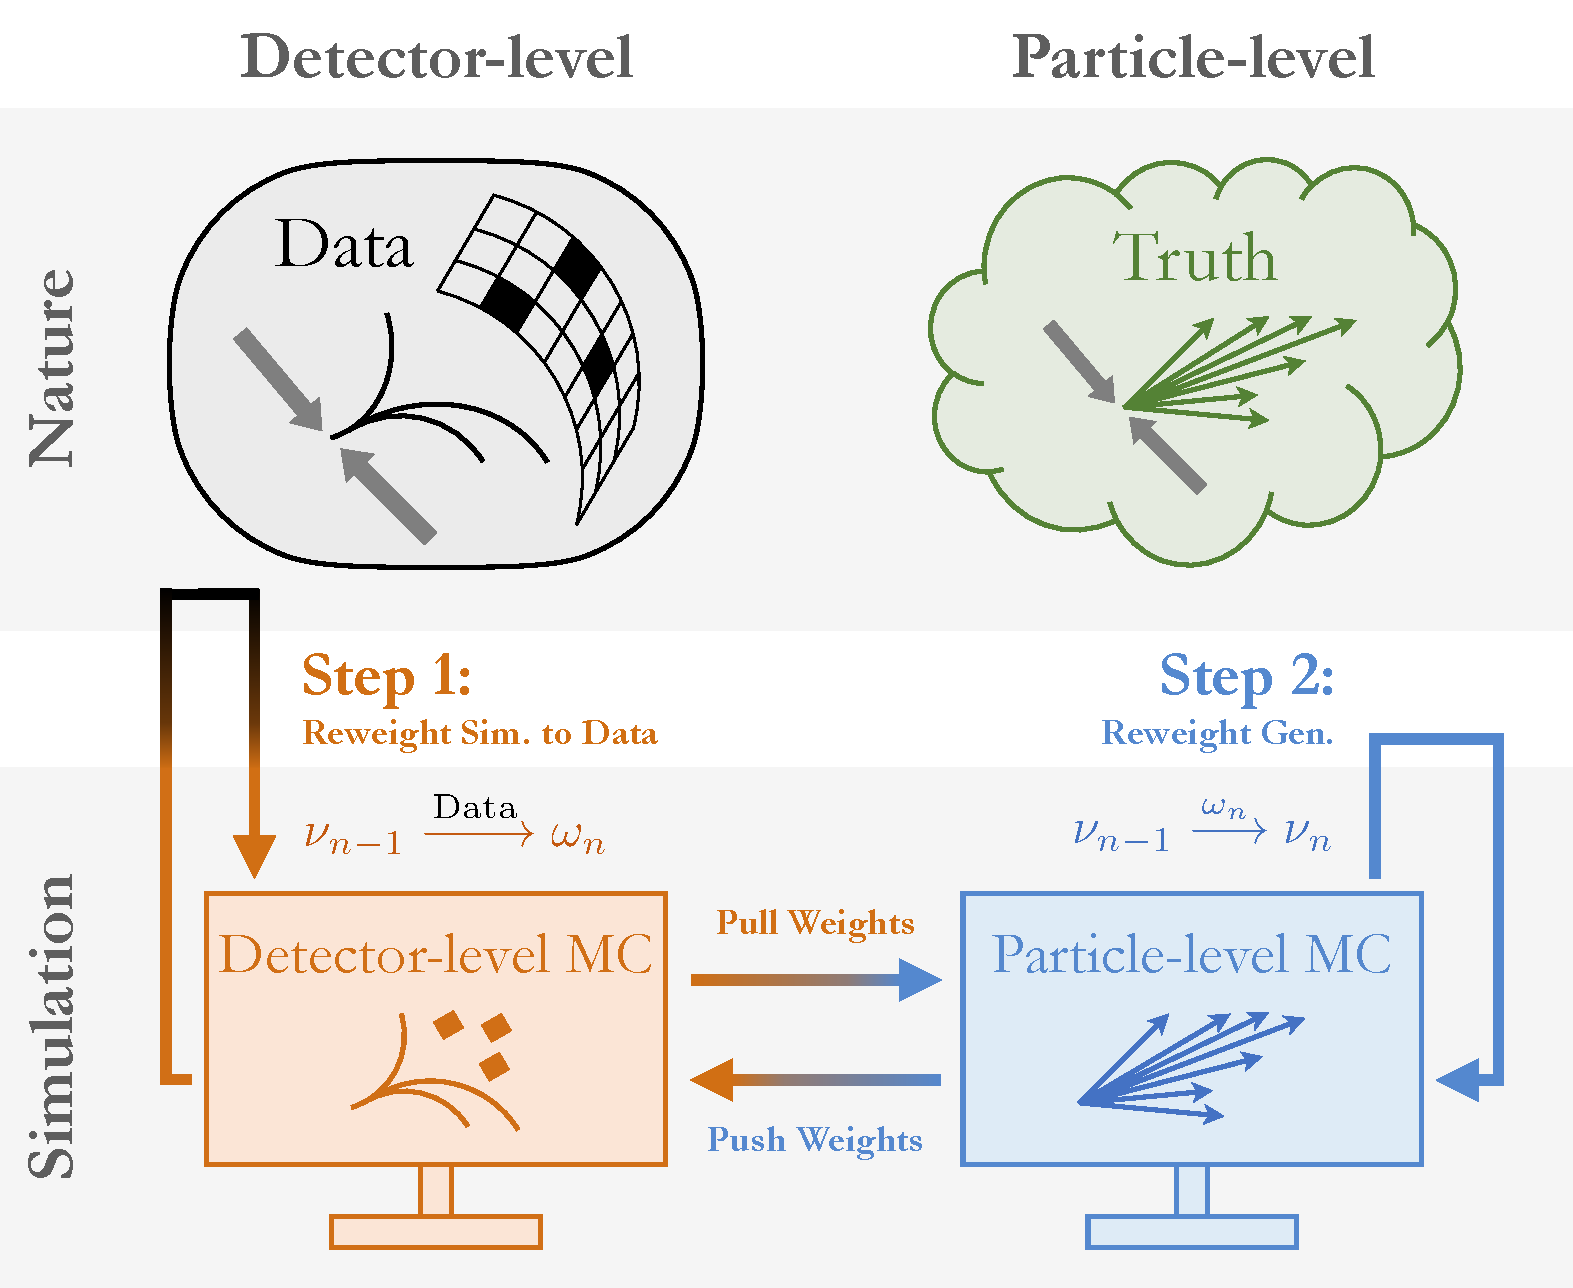
\includegraphics[width=0.6\textwidth]{Figures/schematic.pdf}
\caption{Figure adapted from Ref.~\cite{1911.09107}.}
\label{fig:omnifoldschematic}
\end{figure}

An effective strategy for implementing the OmniFold protocol is to use neural networks as reweighting functions.  A reweighting function is simply a ratio of two probability densities.  It is a fact that the optimal classifier between two event samples is the same quantity - the likelihood ratio (or any monotonic function of it).  Therefore, we build a reweighting function by training a classifier and properly interpreting the output. 
In particular, a classifier $f$ trained using the standard binary cross entropy loss function on events with features $\vec{x}_i$ and event weights $w_i$
%
\begin{align}
\label{eq:binarycrossentropy}
        f^*=\argmin_f~~-\sum_{i\in\text{dataset 1}}w_i \log(f(\vec{x}_i)) -\sum_{i\in\text{dataset 2}} w_i\log(1-f(\vec{x}_i)),
\end{align}
%
has the property\footnote{This fact is well-known~\cite{hastie01statisticallearning,sugiyama_suzuki_kanamori_2012} and also has been used in many contexts in high-energy physics~\cite{2010.03569,1907.08209,Stoye:2018ovl,Hollingsworth:2020kjg,Brehmer:2018kdj,Brehmer:2018eca,Brehmer:2019xox,Brehmer:2018hga,Cranmer:2015bka,Badiali:2020wal,Andreassen:2020nkr,Andreassen:2019cjw,Fischer-ACAT2019}.} that asymptotically (i.e.\ with enough training data, flexible enough network architecture and training):
%
\begin{align}
\frac{f^*(\vec{x})}{1-f^*(\vec{x})}\propto \frac{p(\vec{x}|\text{dataset 1})}{p(\vec{x}|\text{dataset 2})}.
\end{align}
%
The proportionality is equality if the two datasets contain the same number of events; however, a constant is not important from the point of view of reweighting.

The power of neural networks is that they are naturally unbinned and can process high-dimensional data.  Furthermore, neural networks can also process variable-length data.  We will refer to the case that the inputs are one-dimensional as UniFold, the case that the inputs are multi- (but fixed-)dimensional as MultiFold, and the case where there are of variable dimension (namely, the raw particle data) as OmniFold.  If it is clear from context, we will simply refer to all of these approaches as OmniFold.

To develop an intuition for how OmniFold operates, the next section compares various approaches in a two-bin example where it is easy to derive the steps analytically.  Following that, we show a Gaussian example where the power of the neural network becomes clear.

\subsubsection{Illustration of Different Methods}

In order to illustrate the OmniFold procedure and how it compares to other techniques, it is useful to consider a simple two-bin example.  Suppose that there are only two possible values at particle-level and detector-level: $(T_1,T_2)$ and $(R_1,R_2)$, respectively.  The random variable $T_i$ is the number of events with a value $i$ at particle level (and similarly for $R_i$).  Further suppose that the detector response is given by:
%
\begin{align}
\Pr(R_1|T_1)&=100\%\,,\\
\Pr(R_1|T_2)&=50\%\,,
\end{align}
%
where $\Pr(x|y)$ is the conditional probability of $x$ given $y$.  The simulation has probability mass $\Pr_\text{MC}(T_i)=50\%$ so that $\Pr_\text{MC}(R_1)=75\%$ and $\Pr_\text{MC}(R_2)=25\%$.   Finally, we observe $\Pr_\text{Data}(R_1)=50\%$ in data.
With the notation used in Eq.~\ref{eq:foldingequation}, this situation is given by
%
\begin{eqnarray}
	\mathbf{R} = \begin{bmatrix} 1 & 0.5\\ 0 & 0.5\end{bmatrix}, & \mathbf{d} = \begin{bmatrix} 0.5\\ 0.5\end{bmatrix}, & \mathbf{c}=\mathbf{f}=\mathbf{1},~~\mathbf{b}=\mathbf{0}.
\end{eqnarray}
%
What do the various method predict for $\Pr_\text{unfolded}(T_1)$?   Before proceeding, note that the correct answer is $\Pr_\text{Data}(T_1)=0$, i.e.\ $\mathbf{t}=[0 1]^\intercal$.

\paragraph{OmniFold}  The first step of OmniFold is to derive weights $\omega_1$ to make the MC match the data.  The weight function is specified by two numbers, one for each of the two bin values.  These weights are given by $\omega_1(R_i)=\Pr_\text{Data}(R_i)/\Pr_\text{MC}(R_i)$, which is $\omega_1(R_1)=2/3$ and $\omega_1(R_2)=2$.  These weights are then pulled back to particle level.  In MC, 50\% of events have $(T_1,R_1)$, 25\% of events have $(T_2,R_1)$ and 25\% of events have $(T_2,R_2)$.   The first two of these types of events get assigned $\omega(R_1)$ and the last one gets assigned $\omega(R_2)$.  Therefore, the weighted particle-level probability mass function is $\Pr_\text{MC,1}(T_1)=1/3$.  The second step of OmniFold derives weights $\nu_1=\Pr_\text{MC,1}(T_i)/\Pr_\text{MC}(T_i)$, which are $\nu_1(T_1)=2/3$ and $\nu_1(T_2)=4/3$.

The above procedure is then repeated using the weights $\nu_1$ pushed to detector-level.  The new detector-level probability mass is given by $\Pr_\text{MC,2}(R_1)=2/3$.  Detector-level weights are derived according to $\omega_2(R_i)=\Pr_\text{Data}(R_i)/\Pr_\text{MC,2}(R_i)$.  Table~\ref{lab:omnifoldexample} shows the evolution of OmniFold over many iterations.

\begin{table}[h!]
\centering
\begin{tabular}{|ccccccc| }
\hline
$i$ & $\omega_i(R_1)$ & $\omega_i(R_2)$ & $\nu_i(R_1)$ & $\nu_i(R_2)$ & $\Pr_\text{MC,$i$}(R_1)$ & $\Pr_\text{MC,$i$}(T_1)$ \\
\hline
0 & 1 & 1 & 1 & 1 & $\sfrac{3}{4}$ & $\sfrac{1}{2}$ \\
1 & $\sfrac{2}{3}$ & $2$ & $\sfrac{2}{3}$ & $\sfrac{4}{3}$ & $\sfrac{2}{3}$ & $\sfrac{1}{3}$ \\
2 & $\sfrac{3}{4}$ & $\sfrac{3}{2}$ & $\sfrac{1}{2}$ & $\sfrac{3}{2}$ & $\sfrac{5}{8}$ & $\sfrac{1}{4}$ \\
\vdots & \vdots & \vdots & \vdots & \vdots & \vdots & \vdots \\
$\infty$ & 1 & 1 & 0 & 2 & \sfrac{1}{2} & 0\\
\hline
\end{tabular}
\caption{The evolution of OmniFold for the simple two-bin example described in the text.}
\label{lab:omnifoldexample}
\end{table}

\paragraph{Conditional GAN Unfolding (CGU)} In the training phase of CGU, one learns $\Pr(T_i|R_j)$ based on the simulation.  In the simple binned case, this probability mass is specified by four numbers.

\begin{align}
\Pr(T_i|R_j)&=\frac{\Pr(R_j|T_i)\Pr(T_i)}{\Pr(R_j|T_1)\Pr(T_1)+\Pr(R_j|T_2)\Pr(T_2)}\\
&=\frac{\Pr(R_j|T_i)}{\Pr(R_j|T_1)+\Pr(R_j|T_2)}\\
&=\left\{\begin{matrix}\sfrac{2}{3} & \text{$i=1$ and $j=1$} \cr 0 & \text{$i=1$ and $j=2$}  \cr \sfrac{1}{3}& \text{$i=2$ and $j=1$}  \cr 1& \text{$i=2$ and $j=2$}  \end{matrix}\right.
\end{align}
%
Applied to data, we would measure
%
\begin{align}
\Pr{}_\text{unfolded}(T_1)&=\Pr(T_1|R_1)\Pr{}_\text{data}(R_1)+\Pr(T_1|R_2)\Pr{}_\text{data}(R_2)=\sfrac{1}{6}\,,\\
\Pr{}_\text{unfolded}(T_2)&=\Pr(T_2|R_1)\Pr{}_\text{data}(R_1)+\Pr(T_2|R_2)\Pr{}_\text{data}(R_2)=\sfrac{5}{6}\,,
\end{align}
%
which is the wrong answer.

\paragraph{Conditional Normalizing Flow Unfolding (CNFU)} In the binned case, this is equivalent to matrix inversion.   The response matrix is

\begin{align}
\mathbf{R}=\begin{pmatrix} 1& \sfrac{1}{2}\cr 0 & \sfrac{1}{2}\end{pmatrix}\implies \mathbf{R}^{-1}=\begin{pmatrix} 1 & -1 \cr 0 & 2\end{pmatrix}\,.
\end{align}
%
Applying $\mathbf{R}^{-1}$ to $(\sfrac{1}{2},\sfrac{1}{2}$) results in $(0,1)$, the correct answer.  There are many undesirable features of matrix inversion, but it does result in an unbiased measurement.

\paragraph{Iterative Bayesian Unfolding (IBU)}

Table~\ref{lab:ibuexample} shows the evolution of IBU over many iterations.  Note that the second column of Table~\ref{lab:ibuexample} is the same as the last column of Table~\ref{lab:omnifoldexample} - this is because OmniFold and IBU are equivalent in the binned case.

\begin{table}[h!]
\centering
\begin{tabular}{|cccccc| }
\hline
$i$ & $\Pr_\text{MC,$i$}(T_1)$ & $\Pr_0(T_1|M_1)$ & $\Pr_0(T_1|M_2)$ & $\Pr_0(T_2|M_1)$ & $\Pr_0(T_2|M_2)$\\
\hline
$0$ & $\sfrac{1}{2}$ & $\sfrac{2}{3}$ & 0 & $\sfrac{1}{3}$ & $1$\\
$1$ & $\sfrac{1}{3}$ & $\sfrac{1}{2}$ & 0 & $\sfrac{1}{2}$ & $1$\\
$2$ & $\sfrac{1}{4}$ & $\sfrac{2}{5}$ & 0 & $\sfrac{3}{5}$ & $1$\\
\vdots & \vdots & \vdots & \vdots & \vdots & \vdots  \\
$\infty$ & 0 & 0 & 0 & 1 & 1\\
\hline
\end{tabular}
\caption{The evolution of IBU for the simple two-bin example described in the text.}
\label{lab:ibuexample}
\end{table}

\subsection{Gaussian Example}

This section shows the unfolding of a one-dimensional Gaussian random variable with a Gaussian noise model.  Figure~\ref{fig:gaussian:inputs} shows the `data' and `simulation'.  The data has a mean of 1 and a standard deviation of 1.5 while the simulation has a mean of 0 and a standard deviation of 1.  In both cases, the distributions are made up of ten million events and the detector effects (noise) are an additive Gaussian with mean 0 and unit variance.

The neural network implemented for reweighting is comprised of 3 layers, with 50 nodes per layer.  Rectified linear units (ReLU) connect the intermediate layers and the output is Softmax.  The training/validation split is 75/25.  The network is trained for 200 epochs with early stopping using a patience of 10\footnote{The training ends if the validation loss is not improved for 10 epochs.  The network weights with the lowest validation loss are restored.}, and the training time is about 5 seconds per epoch on an NVIDIA Quadro RTX 6000 GPU. The batch size is $10^5$.  All neural networks are implemented using \textsc{Keras}~\cite{keras} with the \textsc{Tensorflow} backend~\cite{tensorflow} and optimized with \textsc{Adam}~\cite{adam}.  Networks are trained using the binary cross entropy loss function described in Eq.~\ref{eq:binarycrossentropy}.

Six iterations resulting in successful unfolding using the OmniFold procedure is demonstrated in Fig.~\ref{fig:gaussian:iterations}.

To model the effects of initial Monte Carlo (MC) generation event weights, we inject artificial initial event weights. Specifically, each event in the particle-level truth and particle-level simulation $x_i$ is given a weight $w_i$ with $w_i$ drawn from $\mathcal{N}(x_i, 1)$; effectively, events further from the origin are more heavily weighted. This results in the distributions shown in Figure~\ref{fig:gaussian:MCinputs}. We then carry out an identical unfolding procedure as described above, simply initializing $\omega_0$ as the initial event weights $w_i$ for simulation.

Again, six iterations resulting in successful unfolding using the OmniFold procedure for the case with initial MC weights injected is demonstrated in Fig.~\ref{fig:gaussian:MCiterations}.

\begin{figure}[h!]
\centering
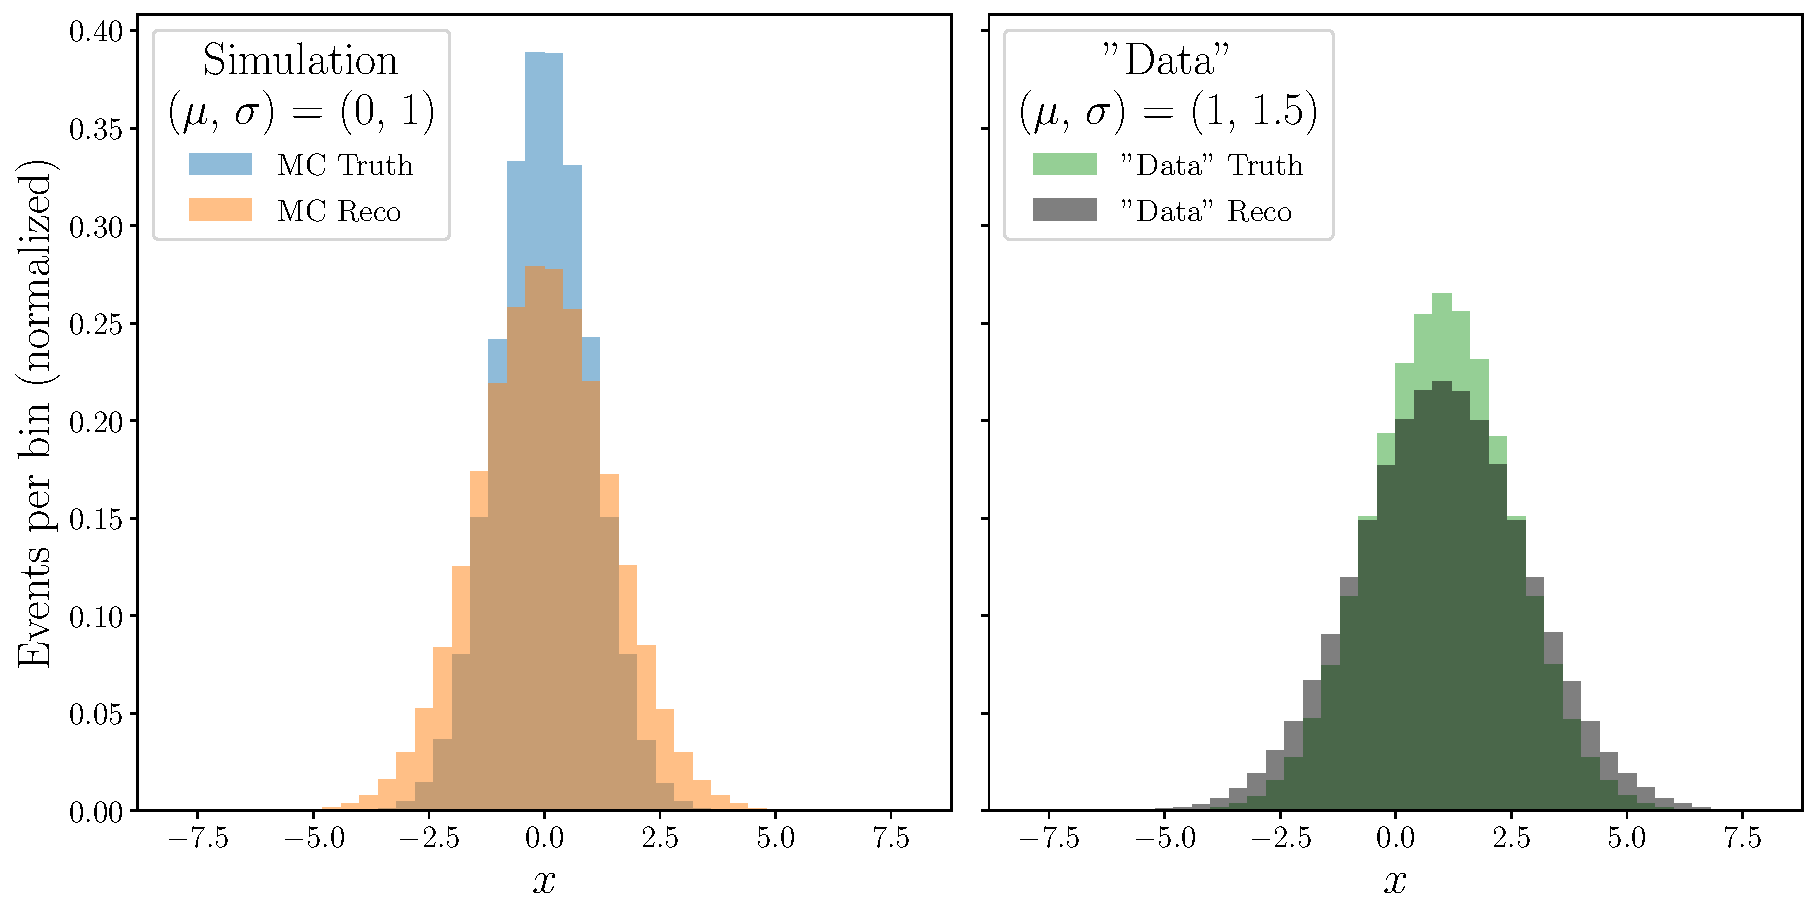
\includegraphics[width=0.6\textwidth]{Figures/GaussianToyExample/GaussianToyExample-Distributions.pdf}
\caption{The `simulation' (left) and `data' (right) for the one-dimensional Gaussian illustration.  The narrower histograms are the particle-level distributions and the wider ones are the detector-level distributions.}
\label{fig:gaussian:inputs}
\end{figure}

\begin{figure}[h!]
\centering
\subfloat[1 iteration]{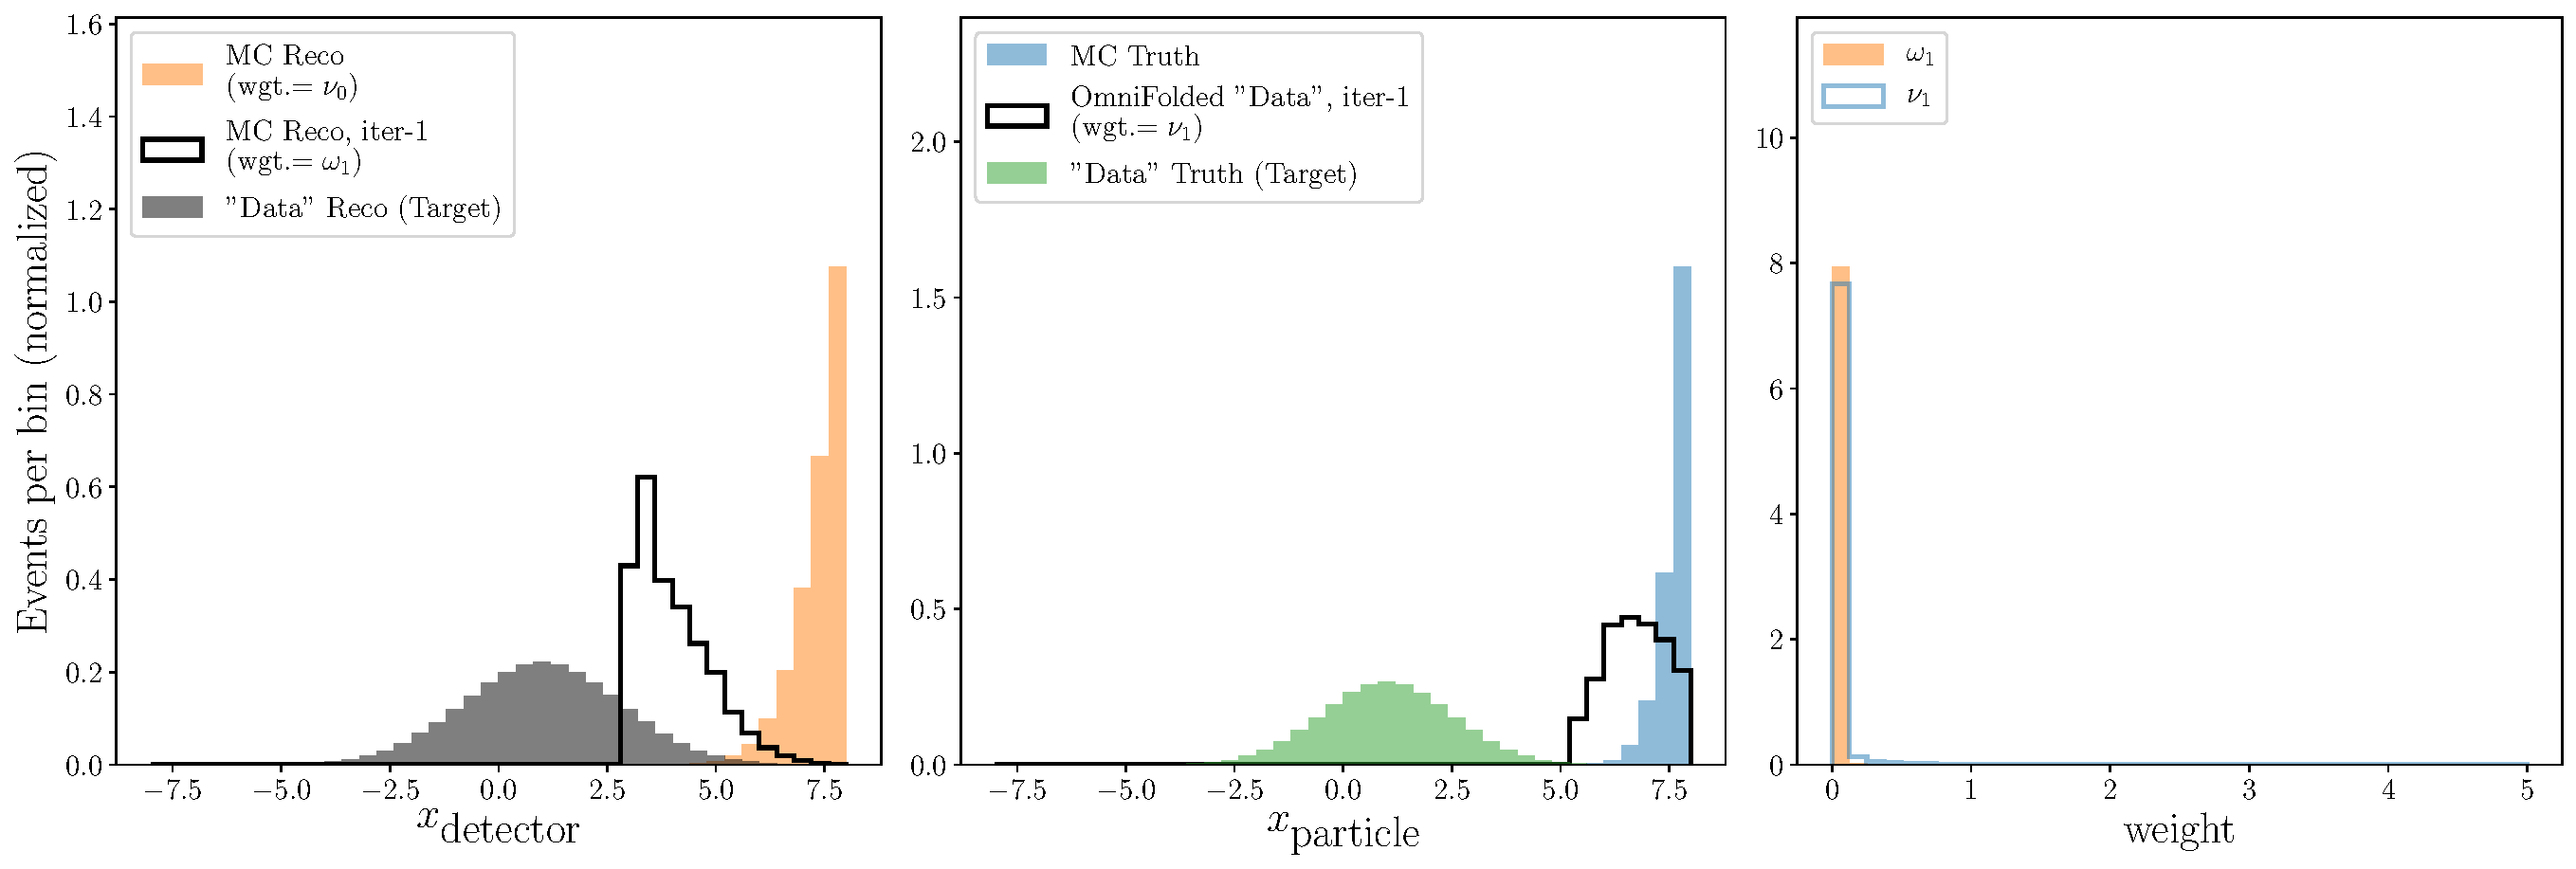
\includegraphics[width=0.45\textwidth]{Figures/GaussianToyExample/GaussianToyExample-UnfoldingResultsIteration01.pdf}}\subfloat[2 iterations]{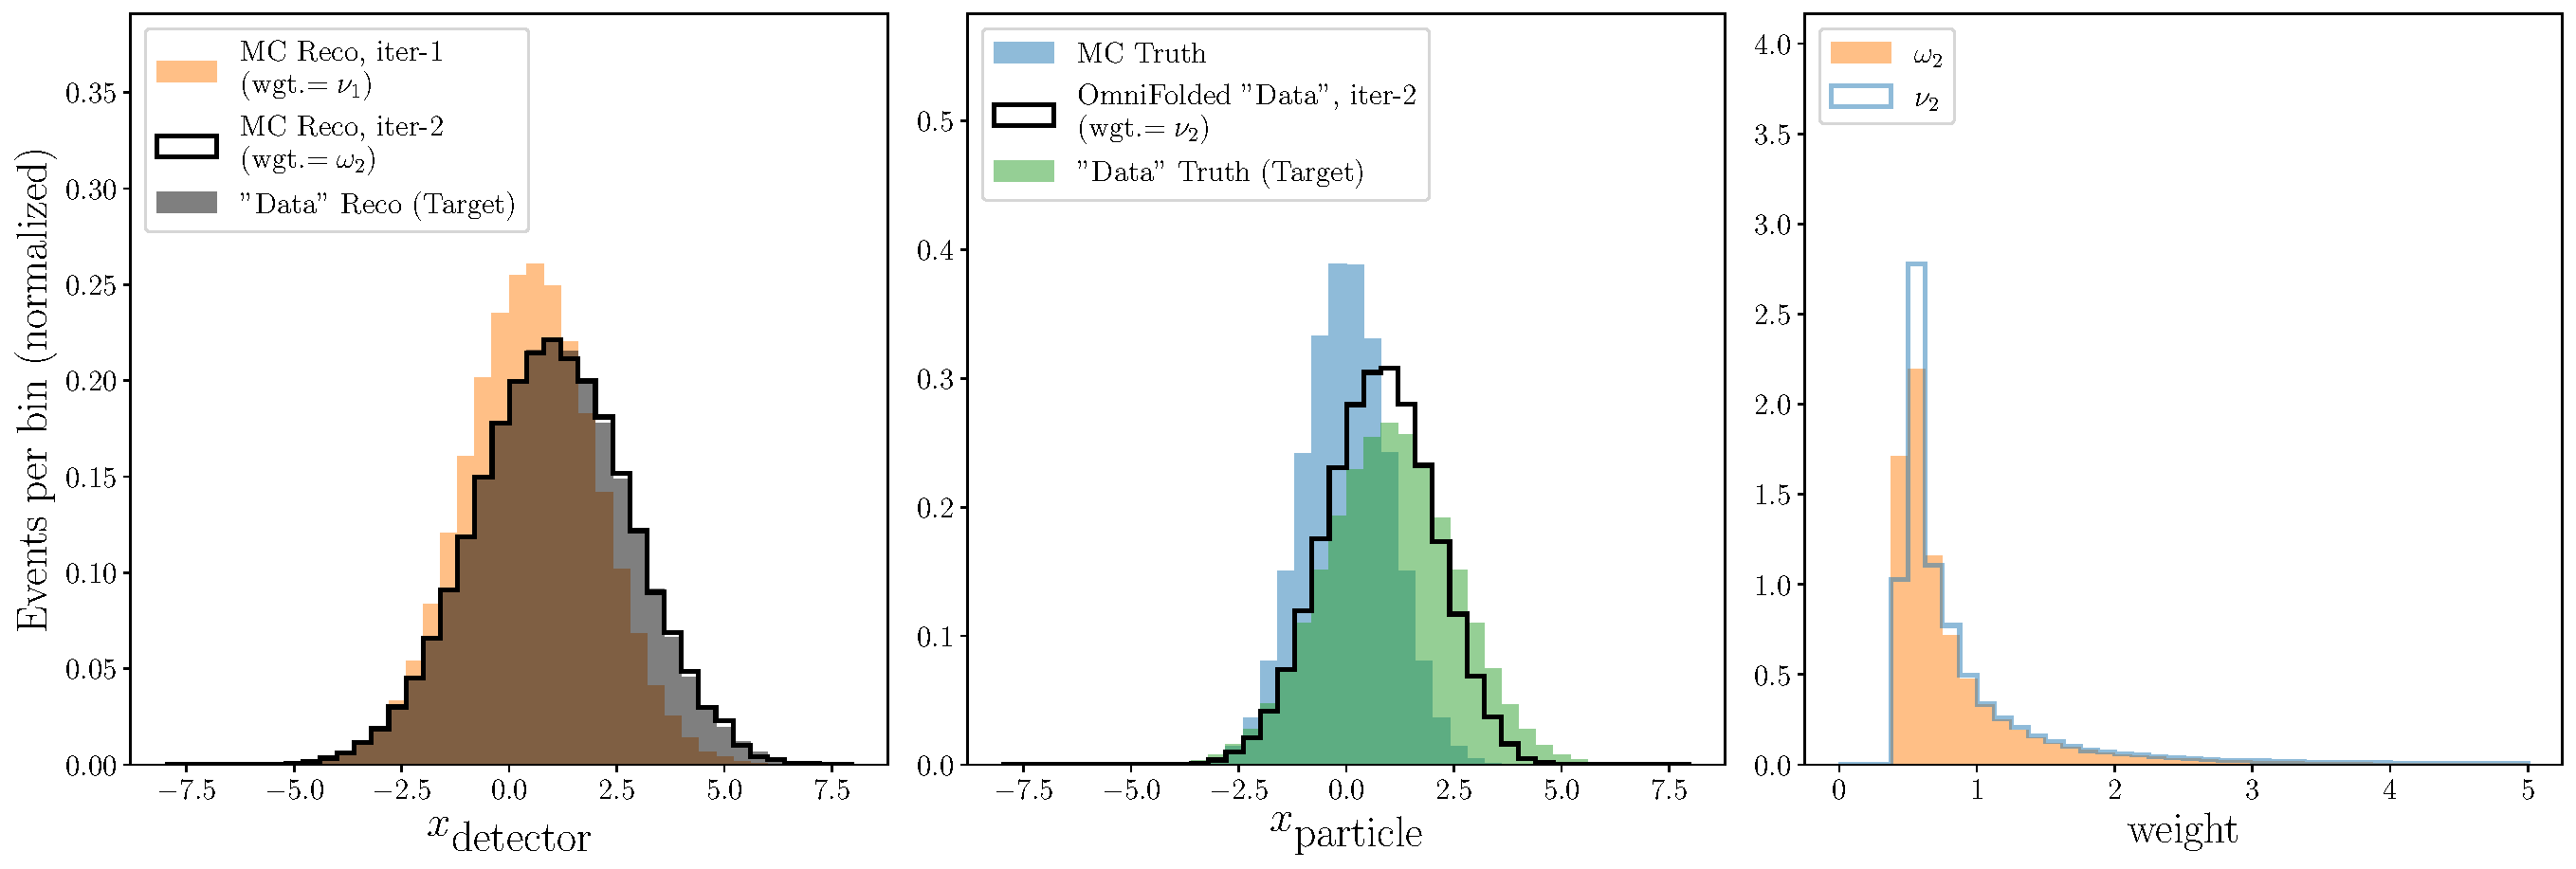
\includegraphics[width=0.45\textwidth]{Figures/GaussianToyExample/GaussianToyExample-UnfoldingResultsIteration02.pdf}}\\
\subfloat[3 iterations]{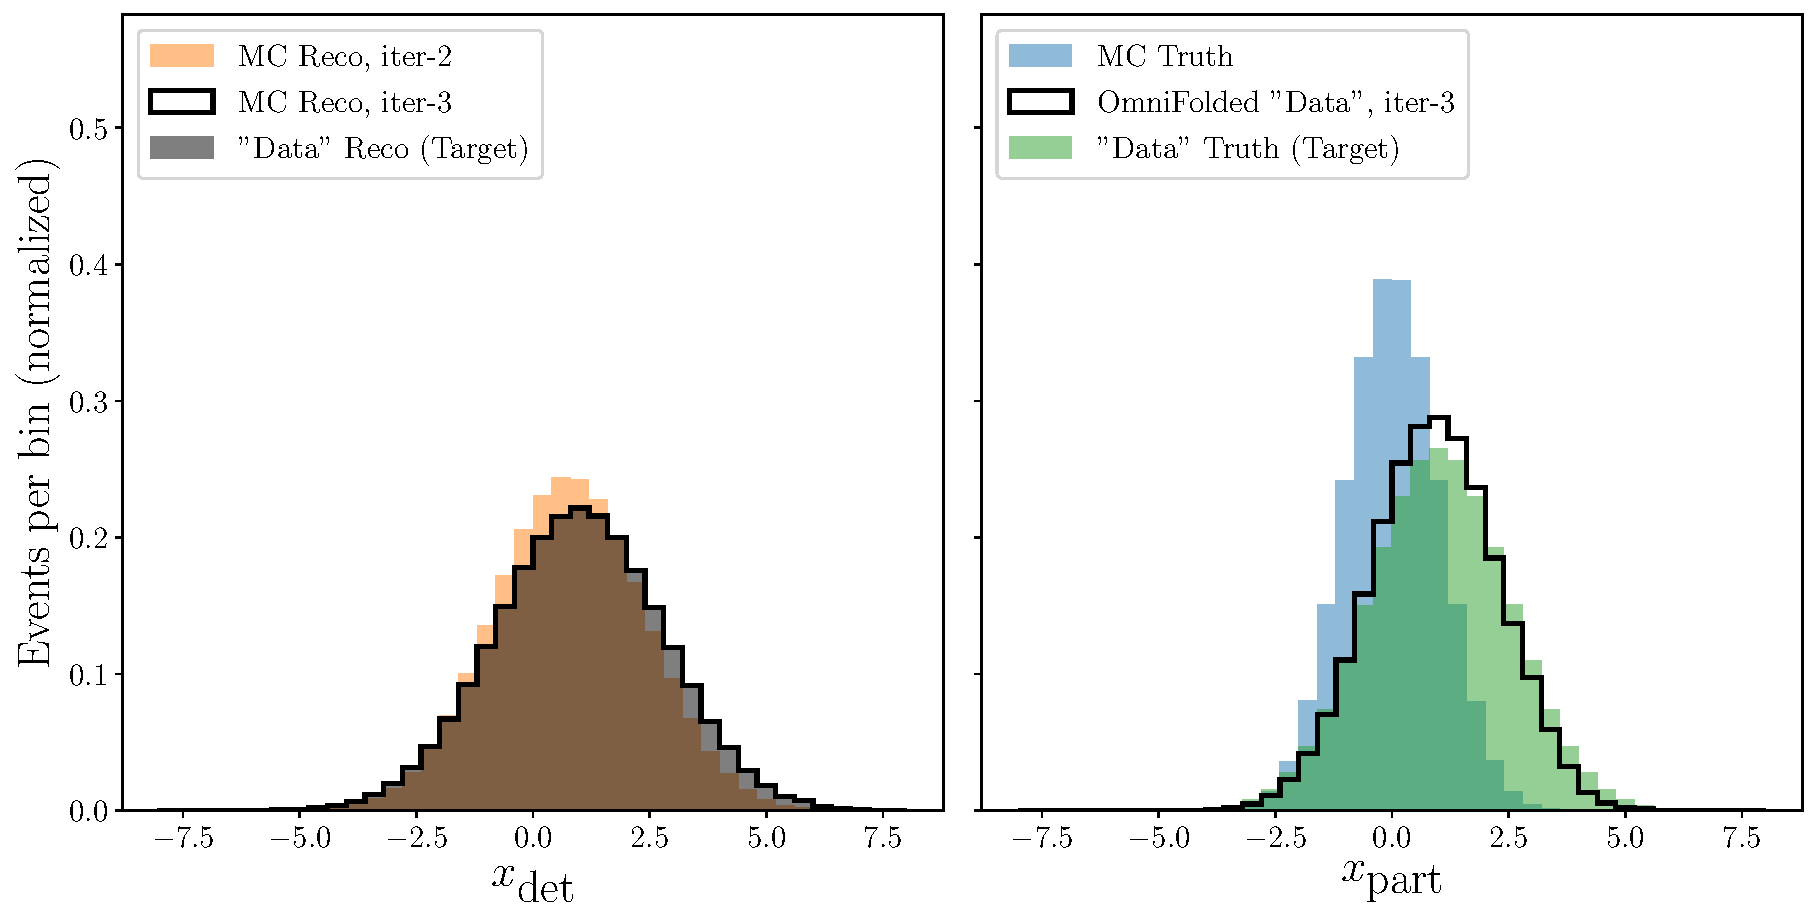
\includegraphics[width=0.45\textwidth]{Figures/GaussianToyExample/GaussianToyExample-UnfoldingResultsIteration03.pdf}}\subfloat[4 iterations]{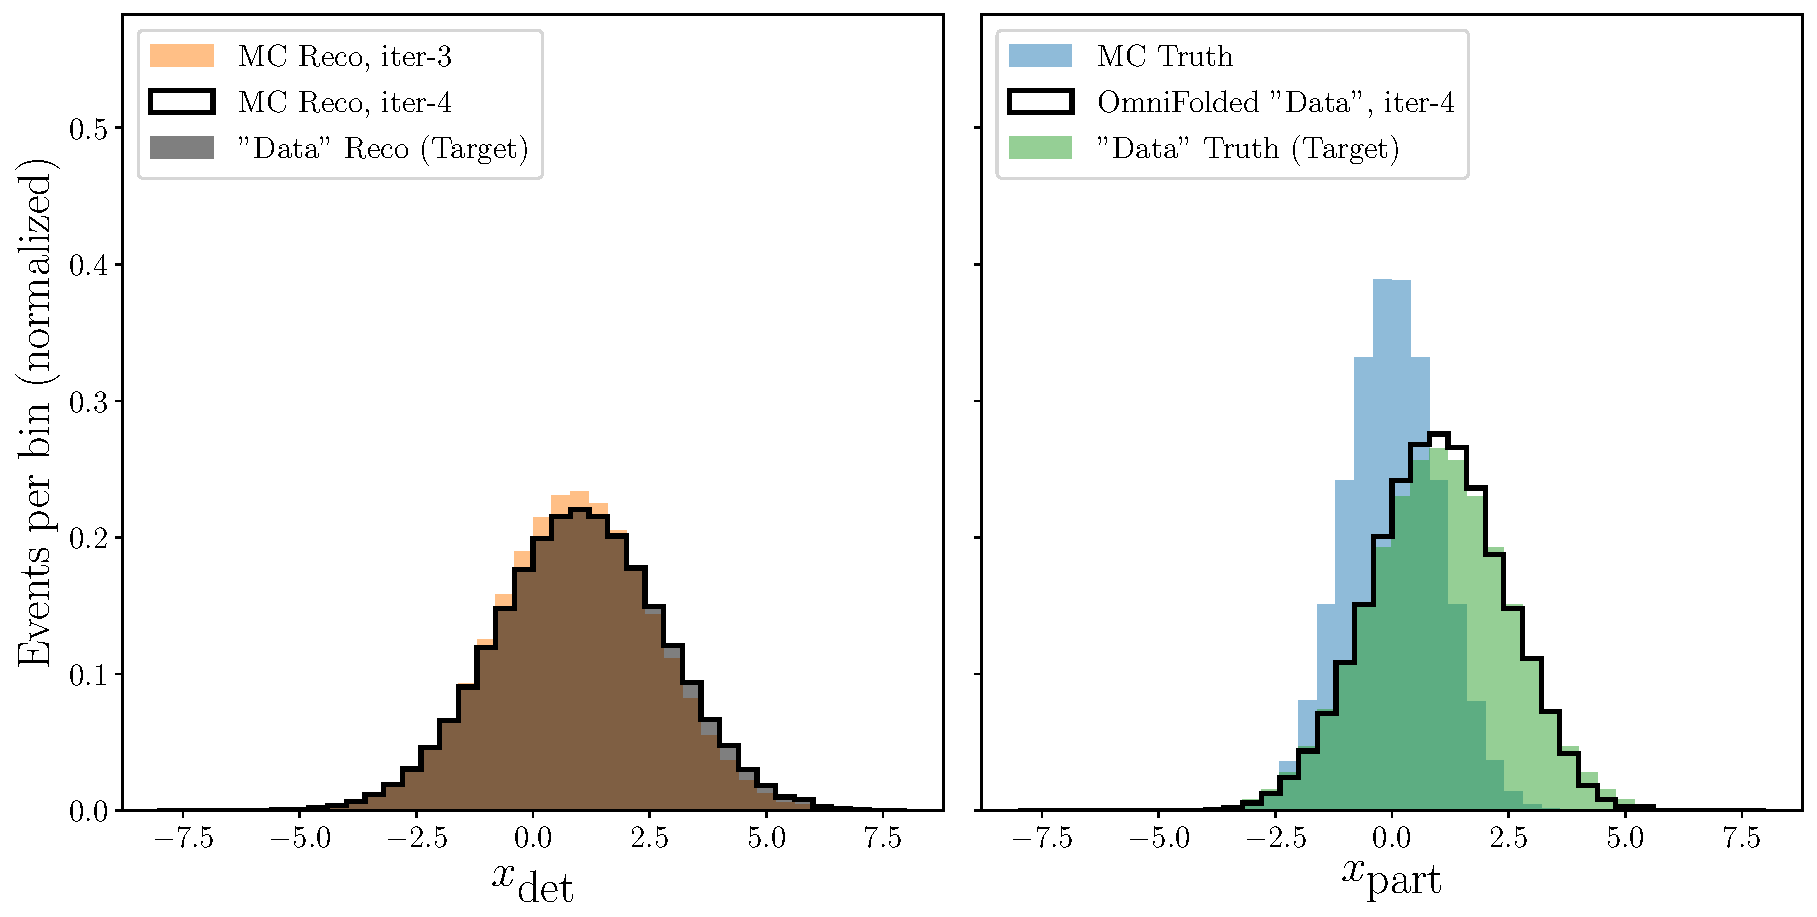
\includegraphics[width=0.45\textwidth]{Figures/GaussianToyExample/GaussianToyExample-UnfoldingResultsIteration04.pdf}}\\
\subfloat[5 iterations]{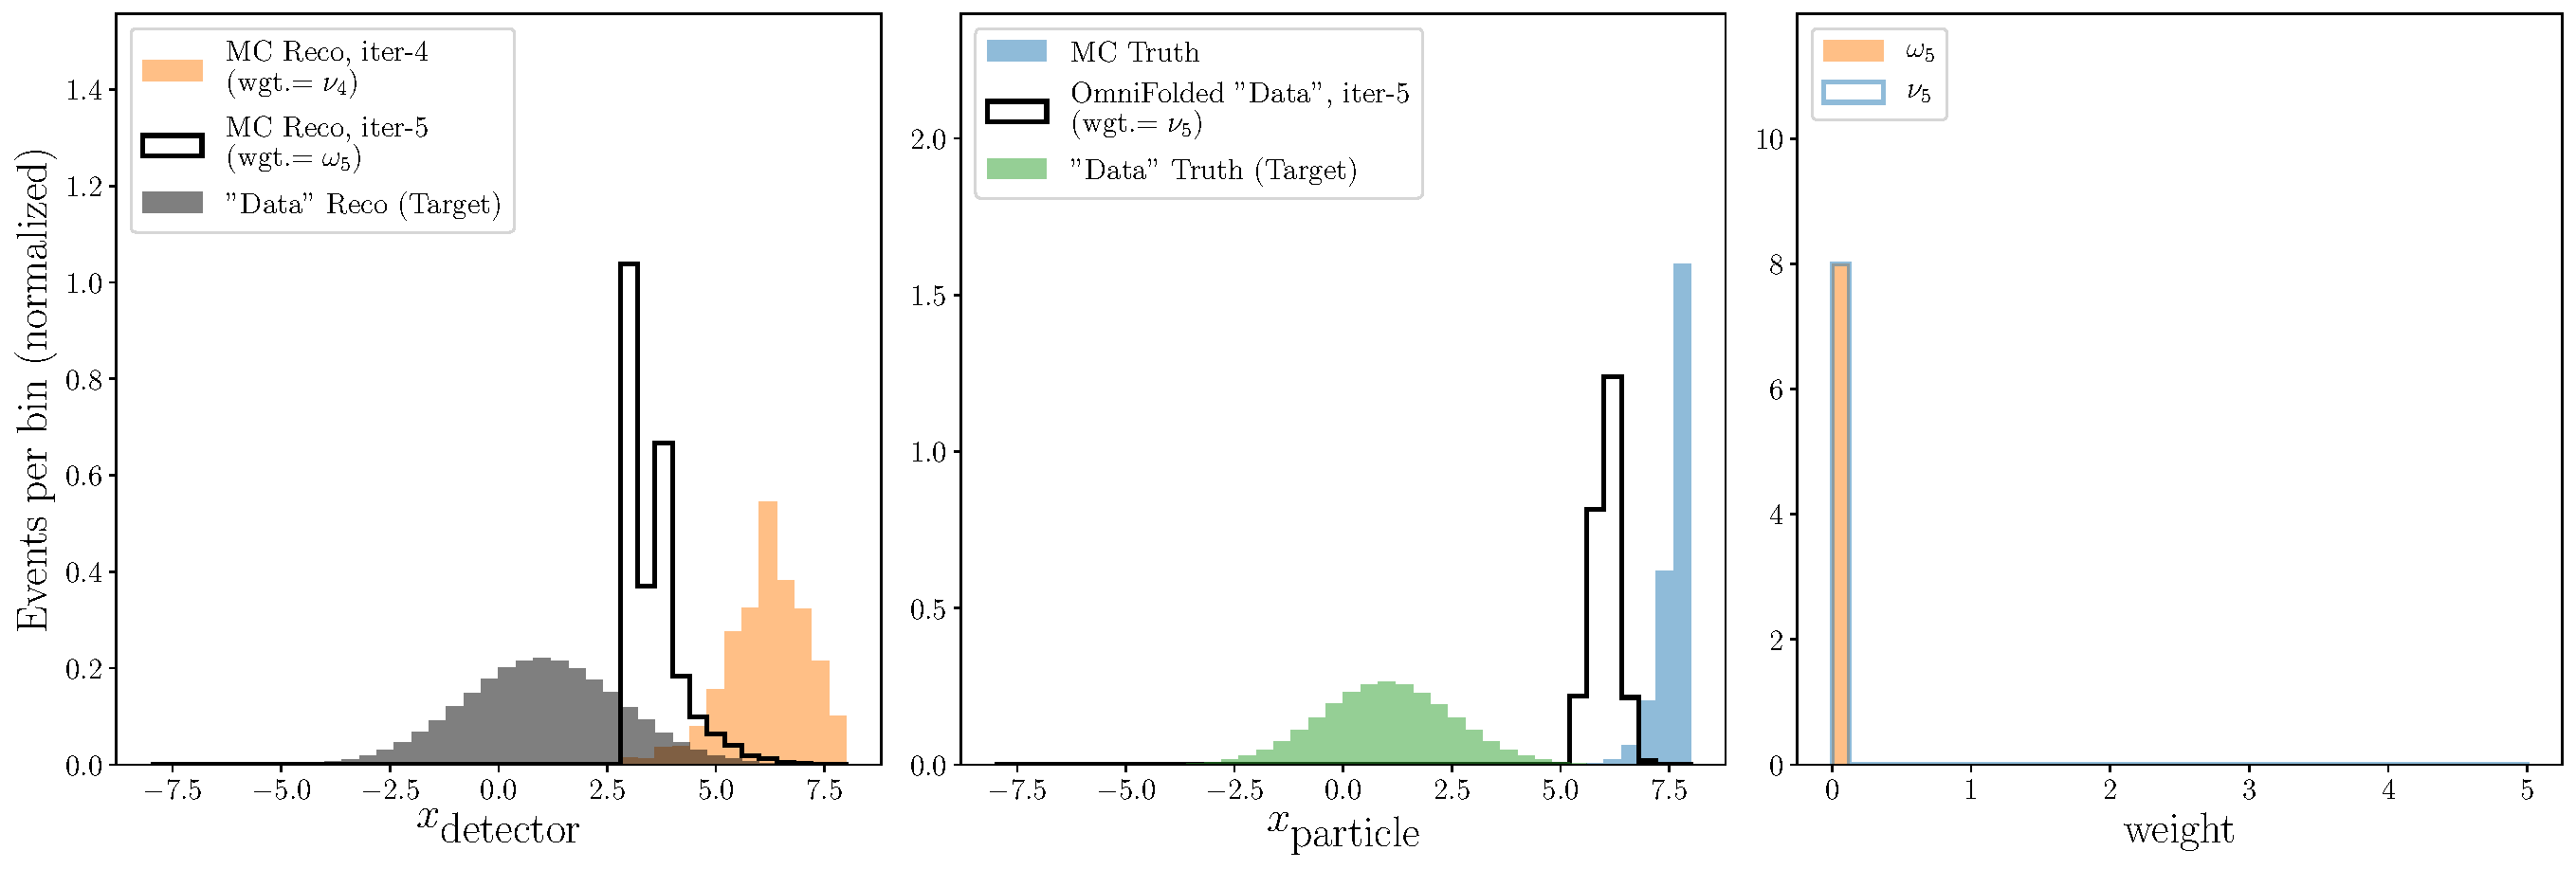
\includegraphics[width=0.45\textwidth]{Figures/GaussianToyExample/GaussianToyExample-UnfoldingResultsIteration05.pdf}}\subfloat[6 iterations]{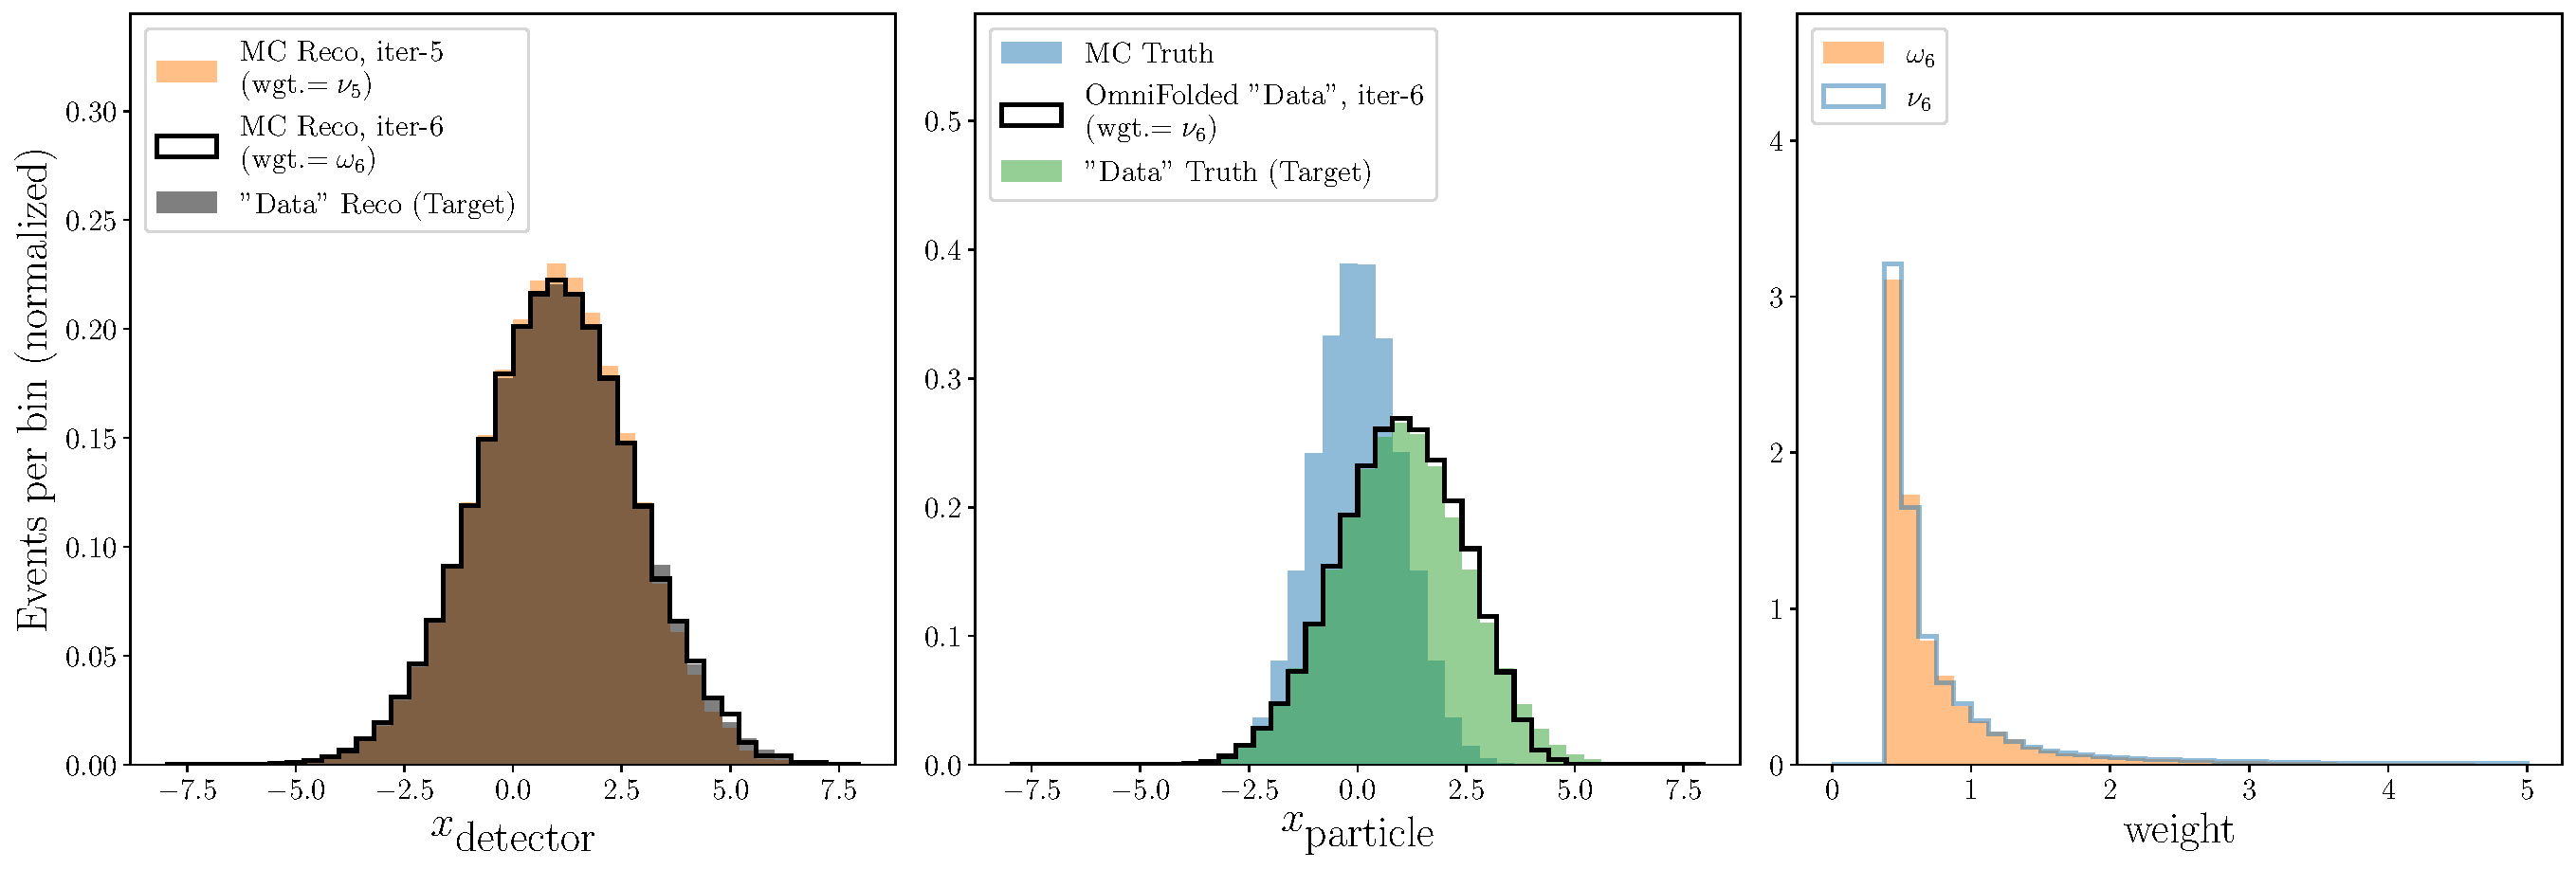
\includegraphics[width=0.45\textwidth]{Figures/GaussianToyExample/GaussianToyExample-UnfoldingResultsIteration06.pdf}}
\caption{An illustration of six iterations of the OmniFold algorithm to the one-dimensional Gaussian example.  For each iteration, the left plot is the detector-level distribution with weights $\omega_n$ and the right plot is the particle-level distribution with weights $\nu_n$.}
\label{fig:gaussian:iterations}
\end{figure}

\begin{figure}[h!]
\centering
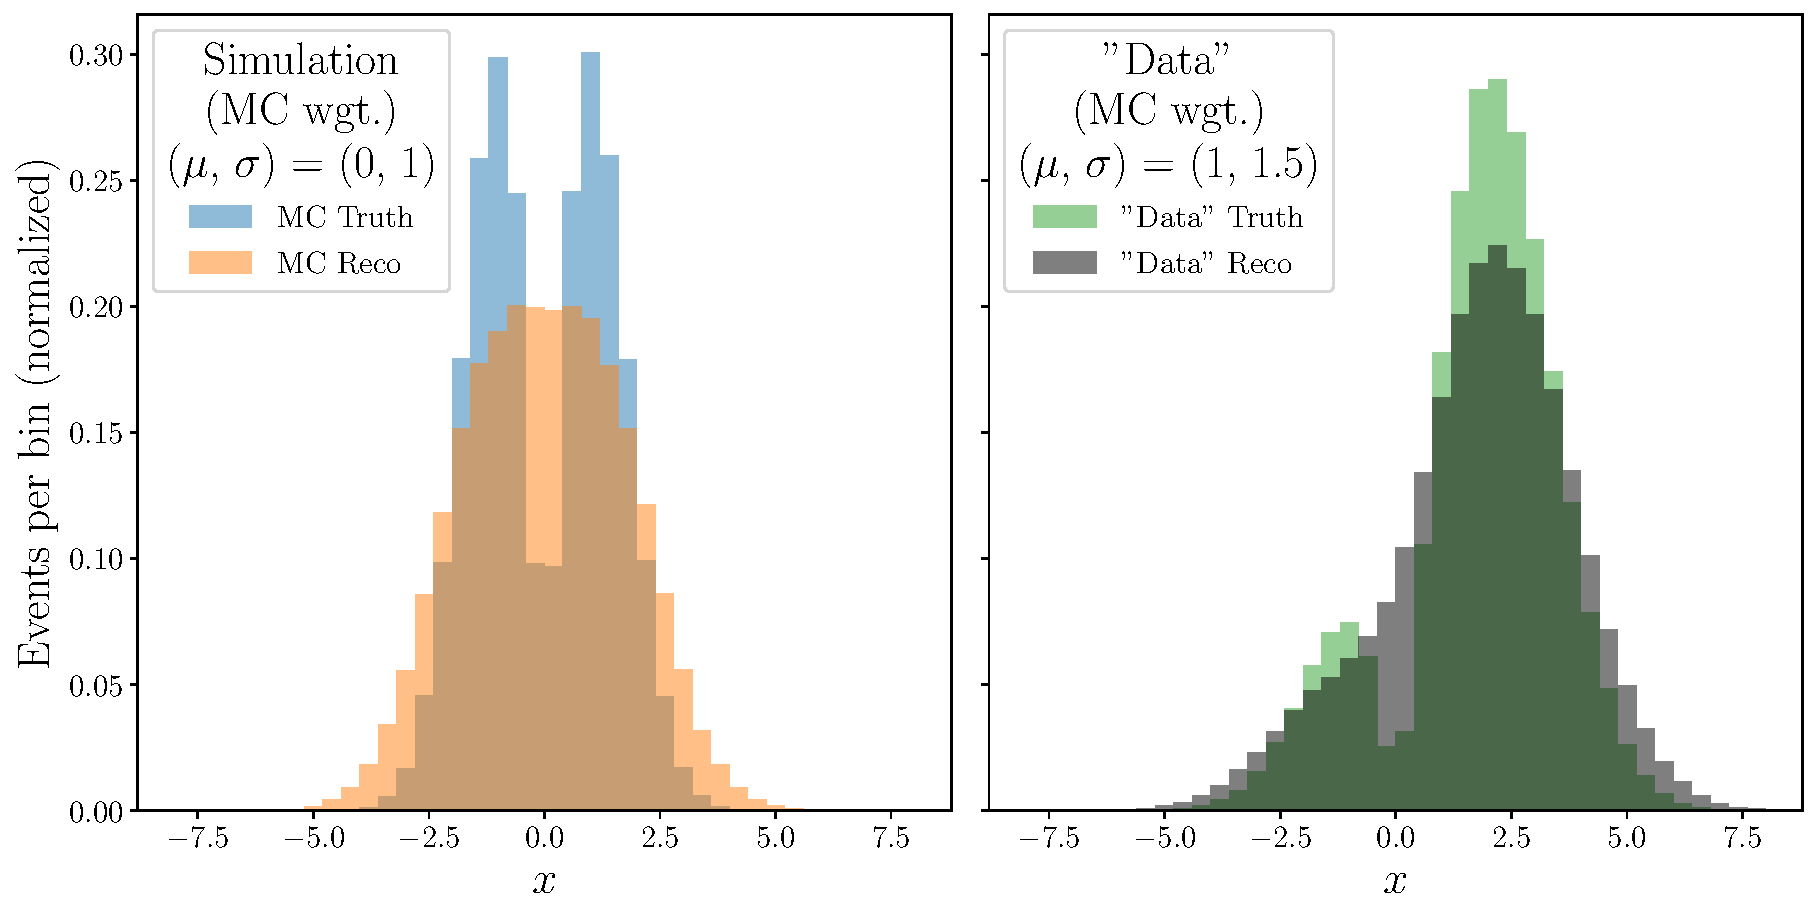
\includegraphics[width=0.6\textwidth]{Figures/GaussianToyExample/GaussianToyExample-MCDistributions.pdf}
\caption{The `simulation' (left) and `data' (right) for the one-dimensional Gaussian illustration with initial MC event weights included.}
\label{fig:gaussian:MCinputs}
\end{figure}

\begin{figure}[h!]
\centering
\subfloat[1 iteration]{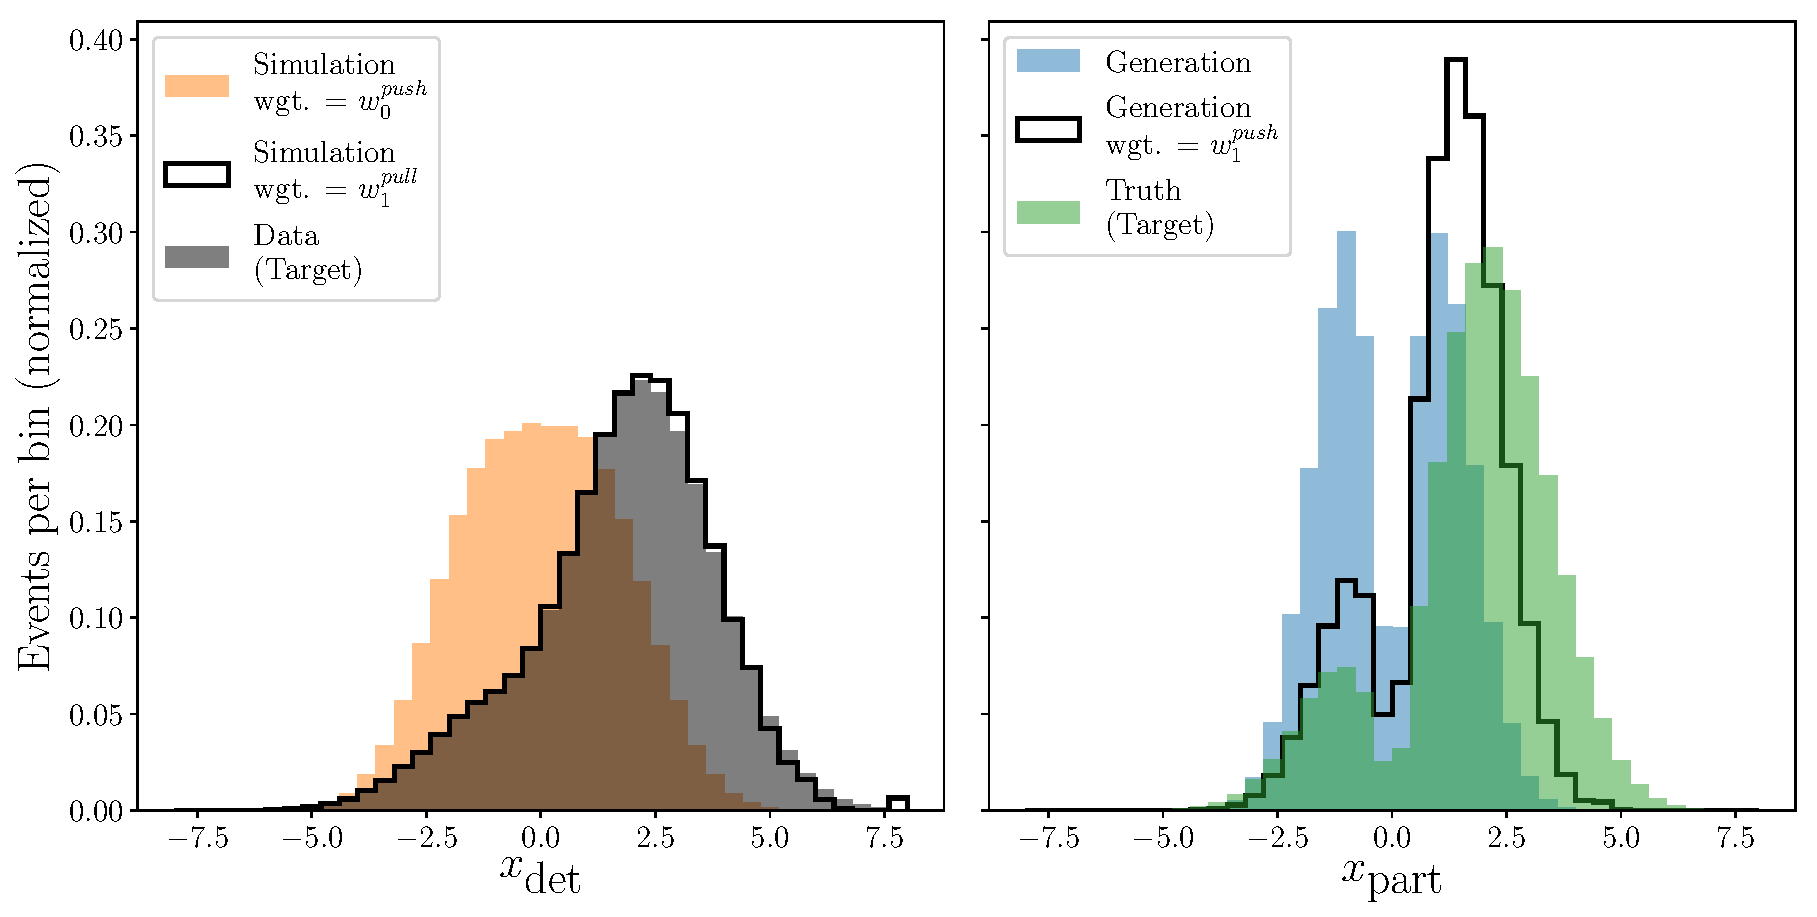
\includegraphics[width=0.45\textwidth]{Figures/GaussianToyExample/GaussianToyExample-MCUnfoldingResultsIteration01.pdf}}\subfloat[2 iterations]{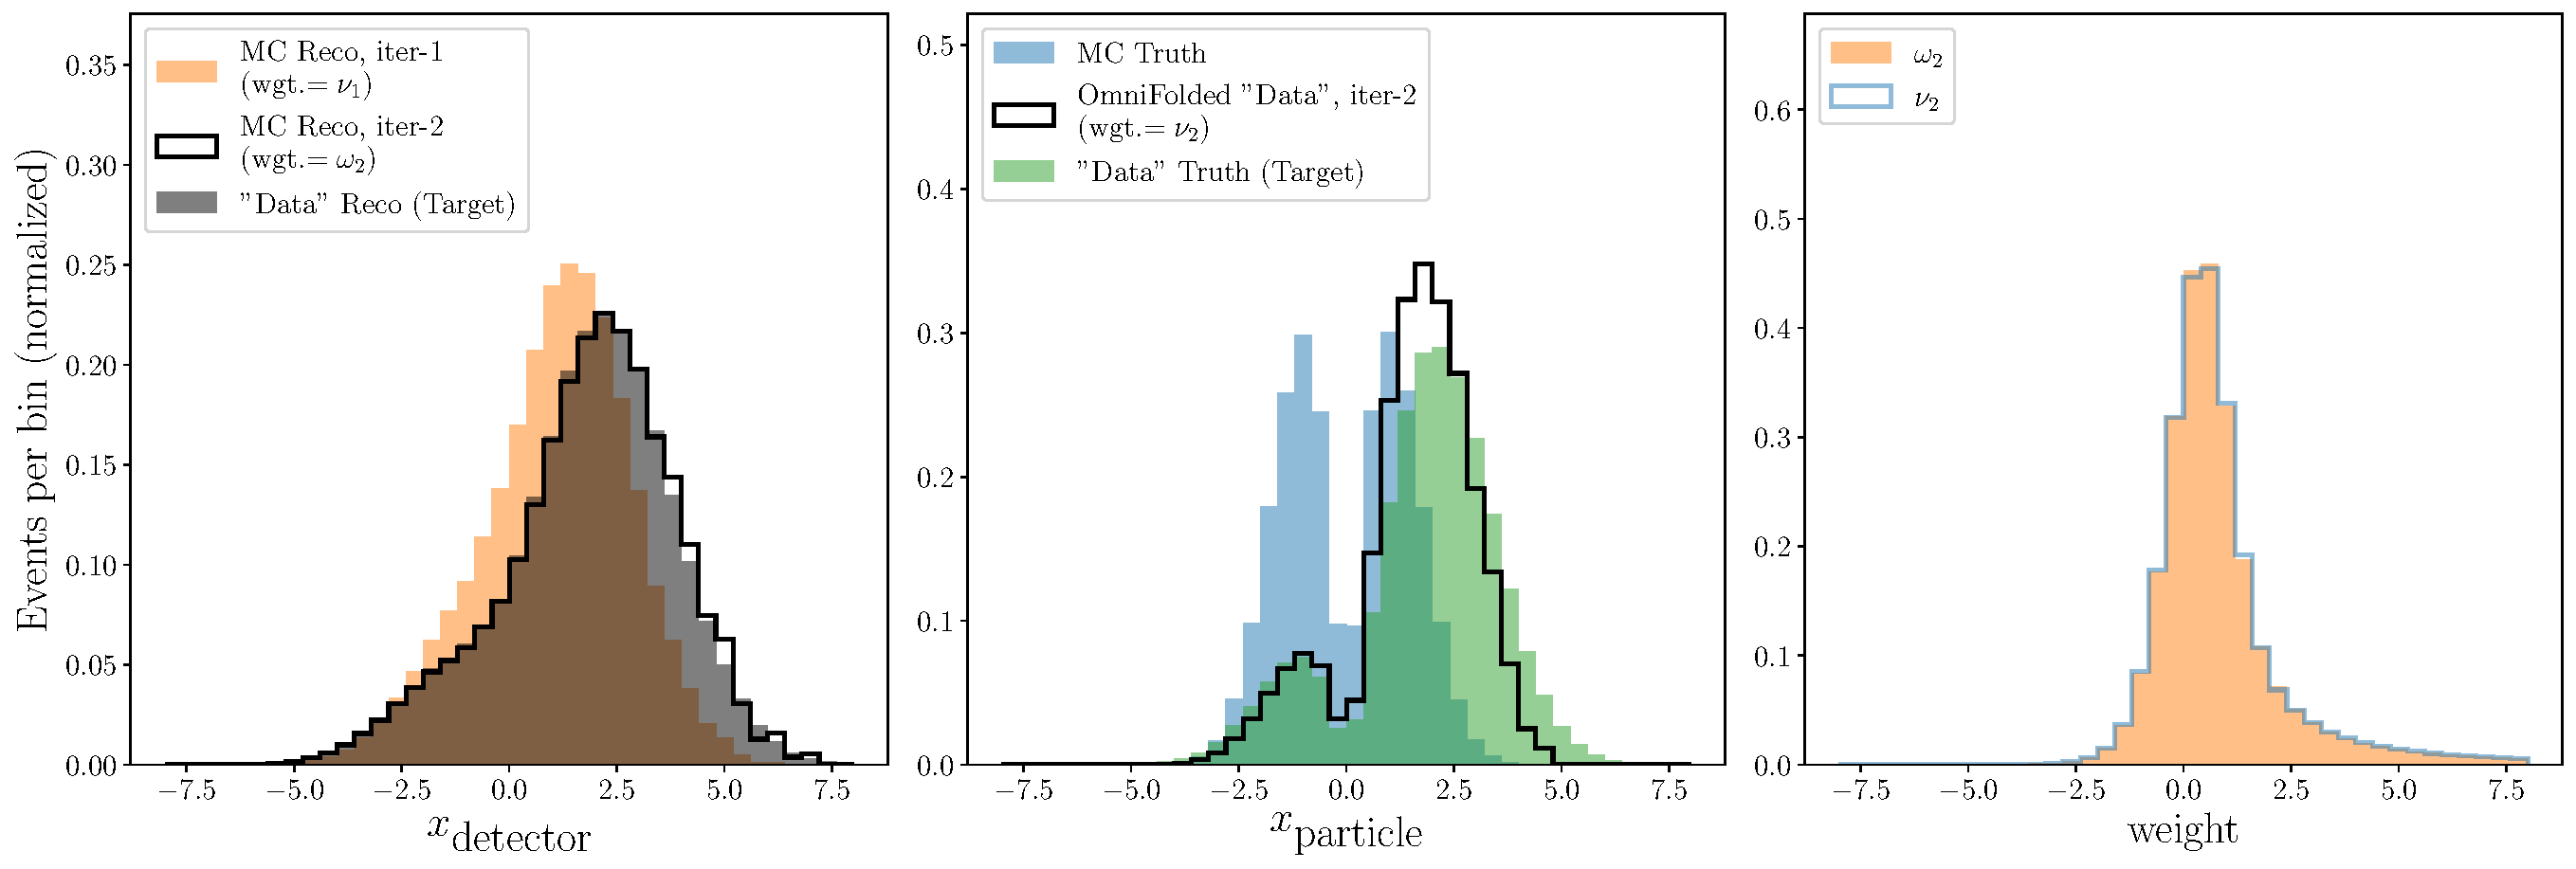
\includegraphics[width=0.45\textwidth]{Figures/GaussianToyExample/GaussianToyExample-MCUnfoldingResultsIteration02.pdf}}\\
\subfloat[3 iterations]{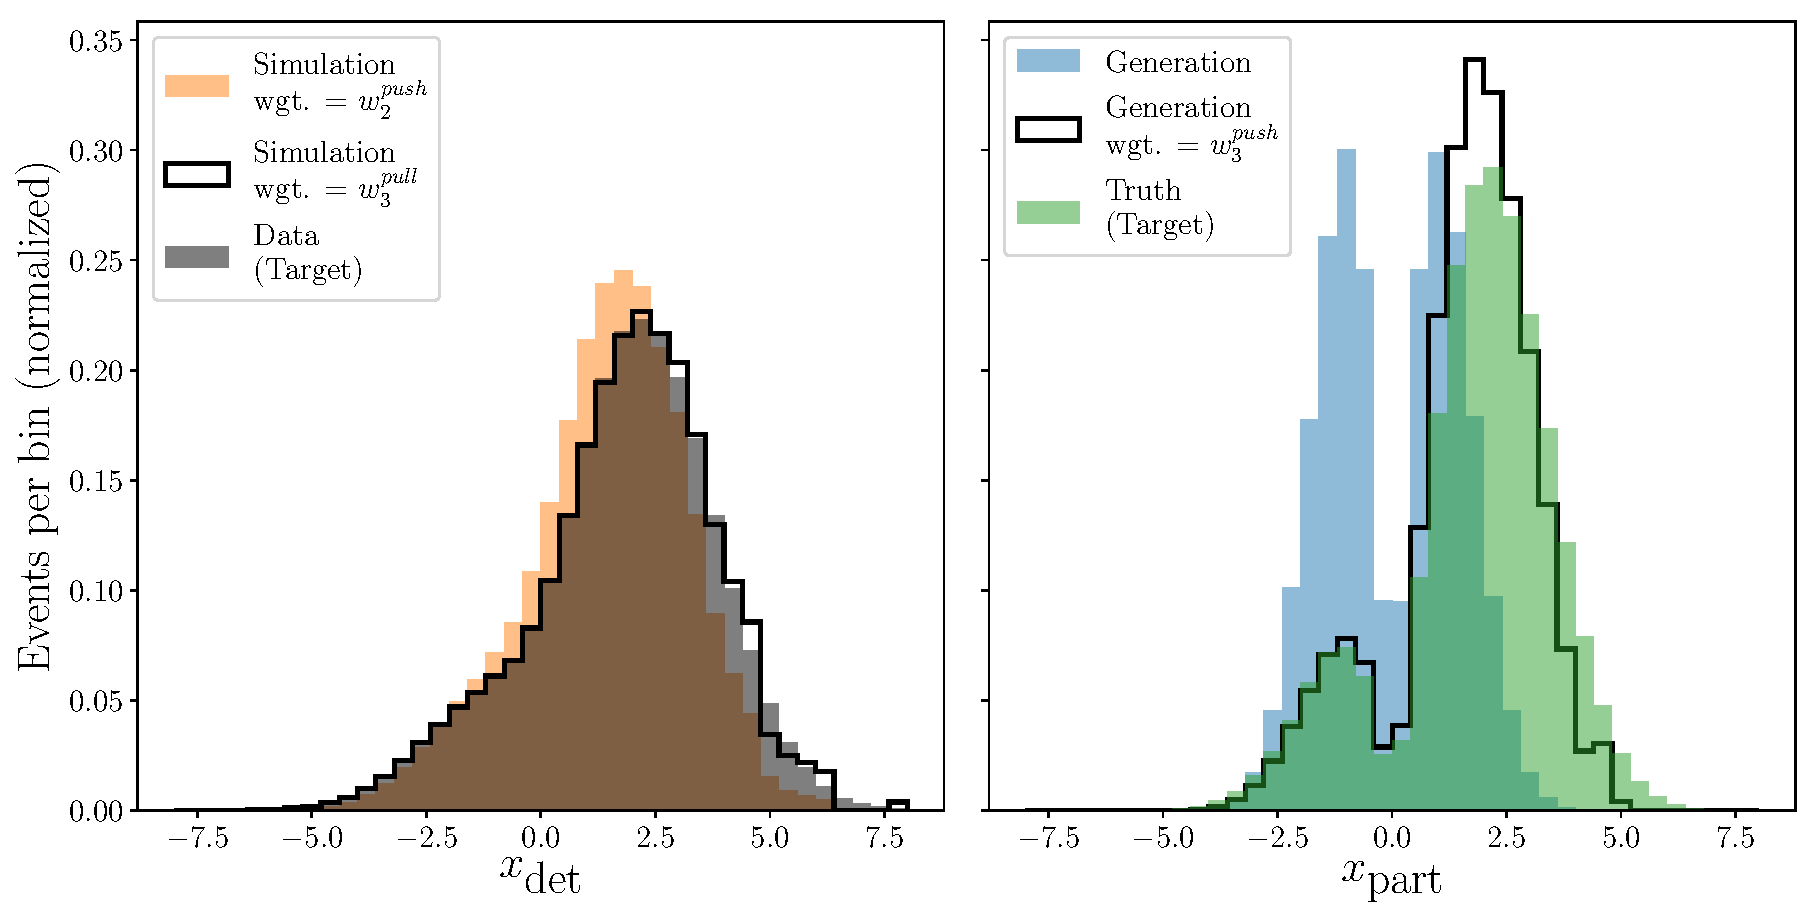
\includegraphics[width=0.45\textwidth]{Figures/GaussianToyExample/GaussianToyExample-MCUnfoldingResultsIteration03.pdf}}\subfloat[4 iterations]{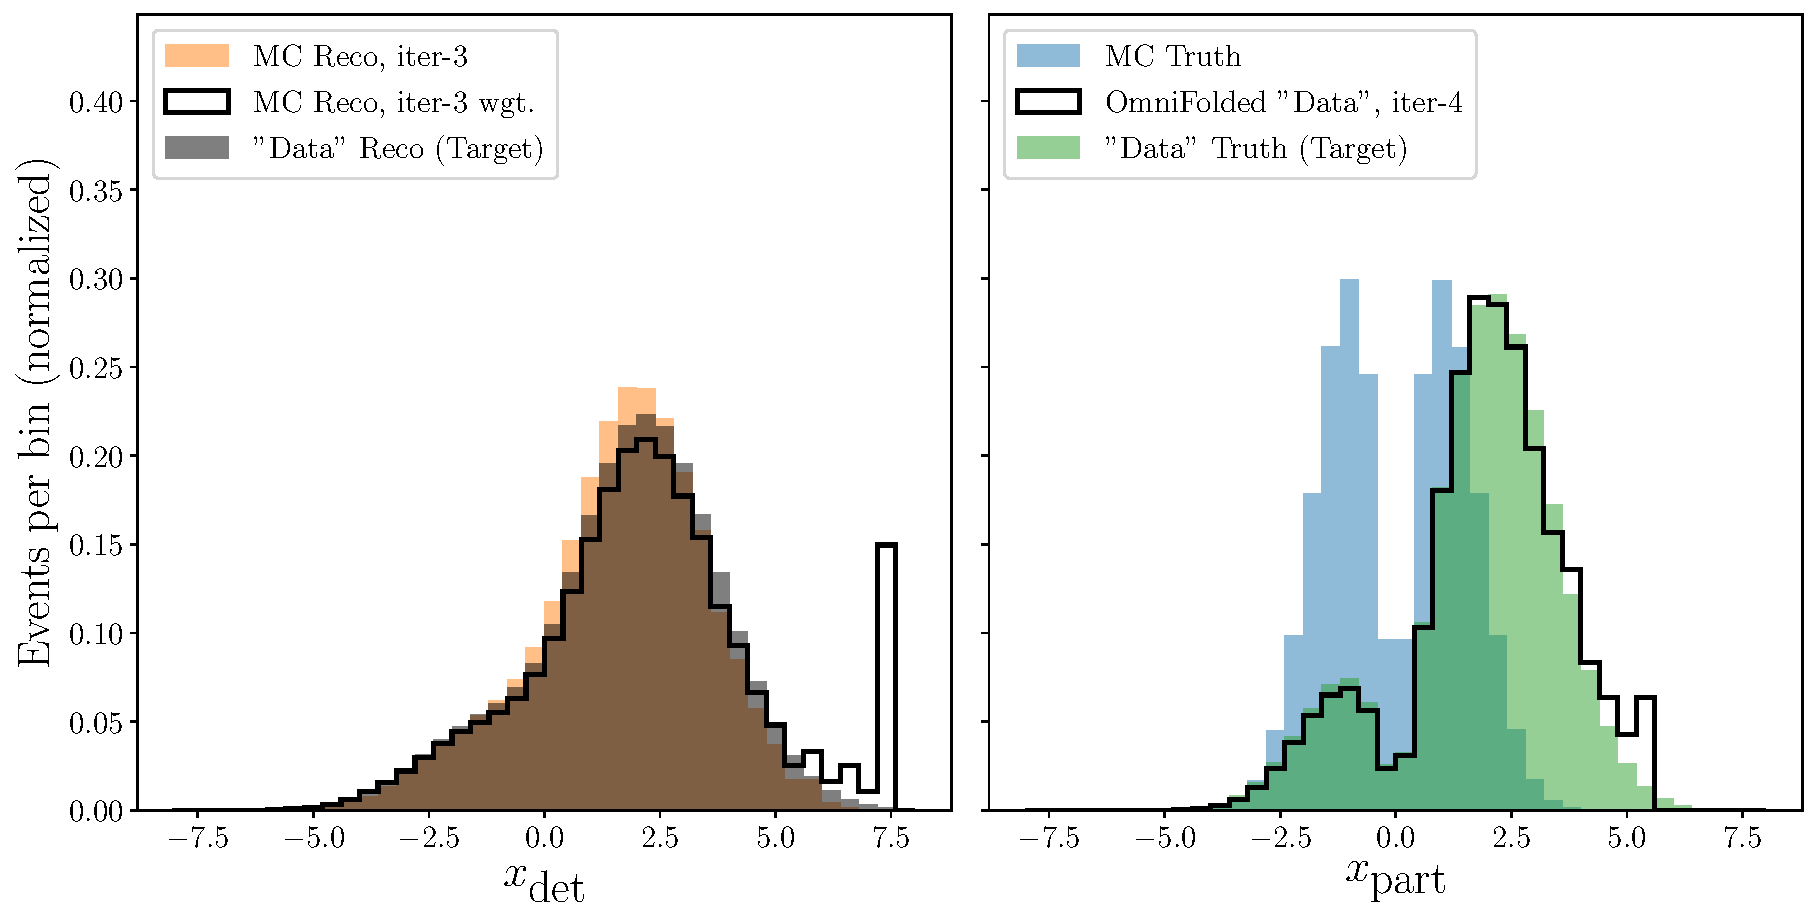
\includegraphics[width=0.45\textwidth]{Figures/GaussianToyExample/GaussianToyExample-MCUnfoldingResultsIteration04.pdf}}\\
\subfloat[5 iterations]{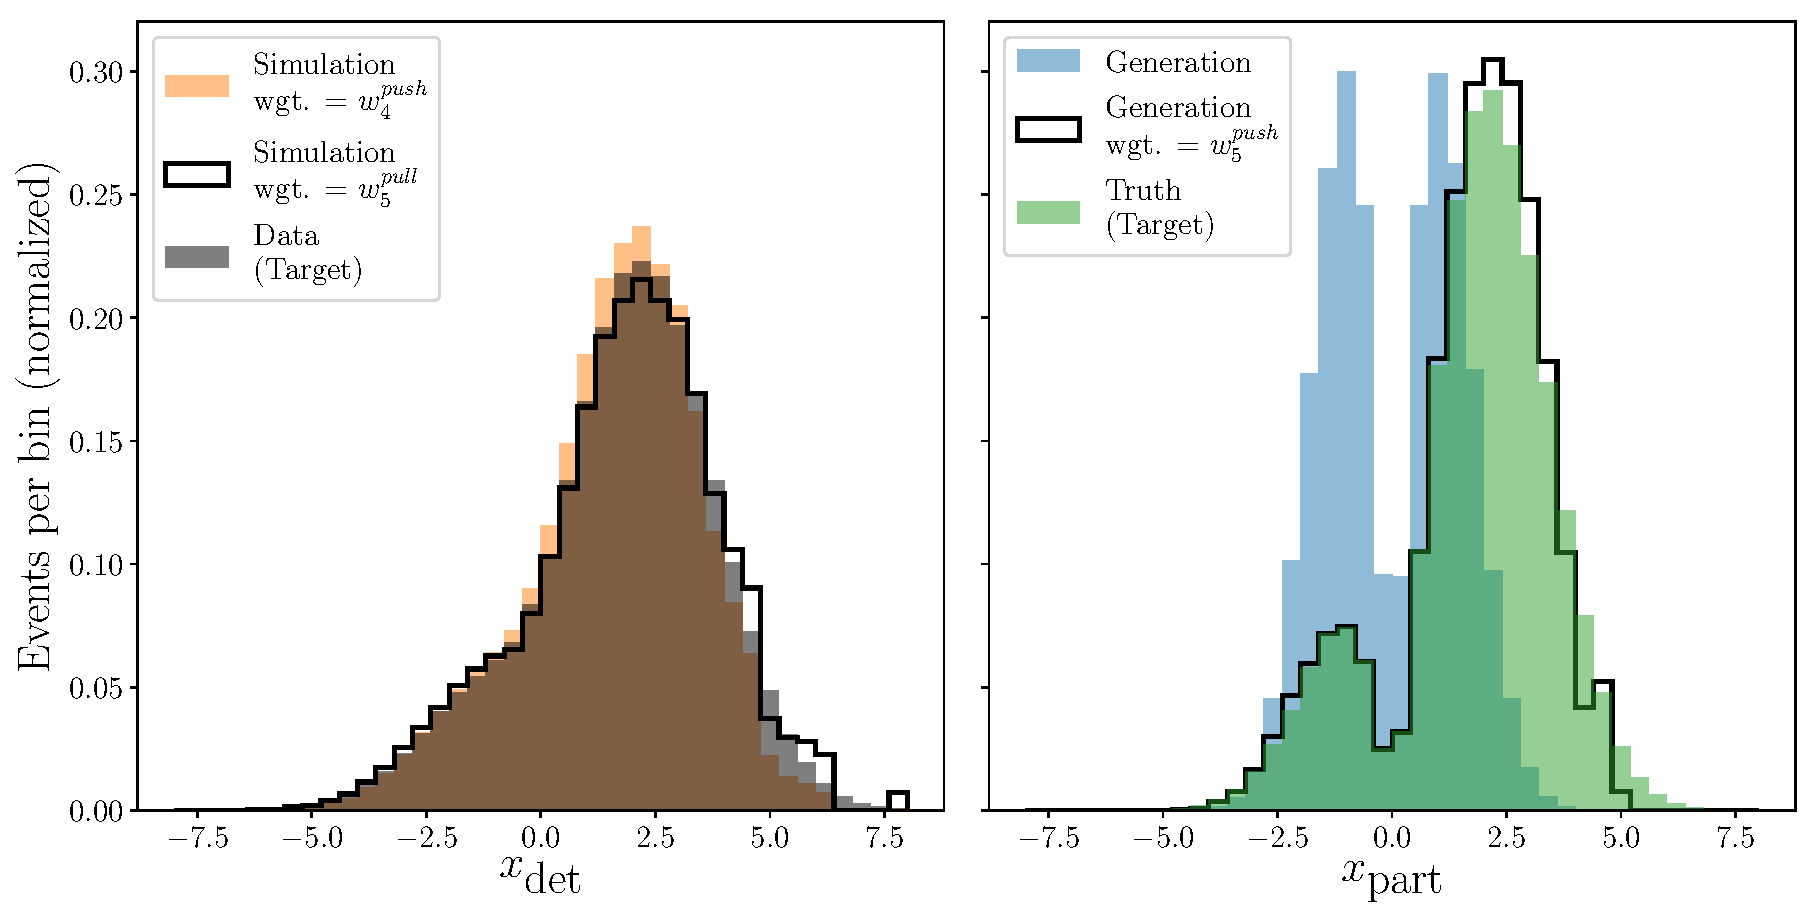
\includegraphics[width=0.45\textwidth]{Figures/GaussianToyExample/GaussianToyExample-MCUnfoldingResultsIteration05.pdf}}\subfloat[6 iterations]{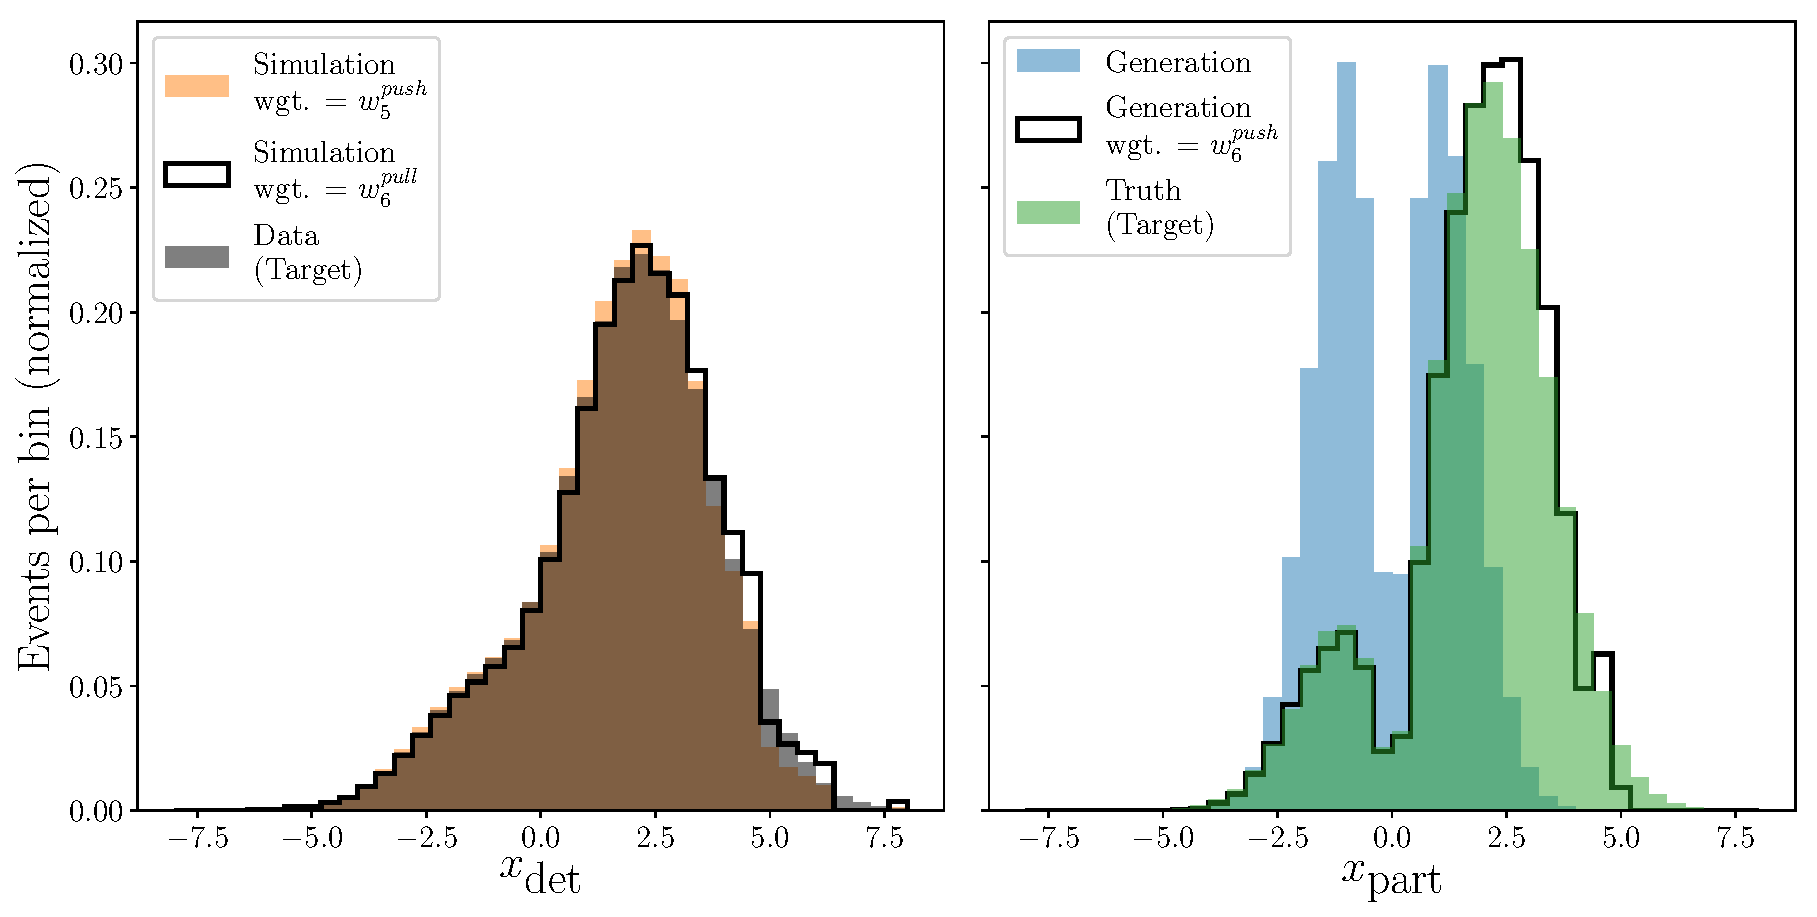
\includegraphics[width=0.45\textwidth]{Figures/GaussianToyExample/GaussianToyExample-MCUnfoldingResultsIteration06.pdf}}
\caption{An illustration of six iterations of the OmniFold algorithm to the one-dimensional Gaussian example with initial MC event weights injected.  For each iteration, the left plot is the detector-level distribution with weights $\omega_n$ and the right plot is the particle-level distribution with weights $\nu_n$.}
\label{fig:gaussian:MCiterations}
\end{figure}

\clearpage

\subsection{OmniFold for ATLAS}

As in the previous section, all neural networks are implemented in \textsc{Tensorflow} and optimized with \textsc{Adam}.  The following sections contain a series of validation studies, starting with a technical closure test in Sec.~\ref{sec:technicalclosure}, a series of artificial stress tests in Sec.~\ref{sec:technicalclosure2}, and then a Pythia-Sherpa comparison in Sec.~\ref{sec:modeldep}.  In each section, we will first show the results on individual observables (UniFold) and then extend the results to multidimensional unfolding.  Note that in all plots, the unfolded result is unbinned, even though histograms with a fixed binning are used for illustration.  The unfolded results can be readily rebinned.

All of the input features are standardized by subtracting the mean and dividing by the per-feature standard deviation.  The neural networks for UniFold and MultiFold have three hidden layers with 50 nodes each using the ReLU activation for internal layers and the sigmoid activation for the last layer.  We train for 200 epochs with early stopping using a patience of 10 epochs.

\subsection{Technical Closure Test}
\label{sec:technicalclosure}

As a technical closure test, we unfold Pythia with itself.  To do this, we take the Pythia sample and randomly label half as `data' and the other half as `simulation'.   The unfolding should converge after one step because the Step 1 and thus Step 2 weights should all be unity.  This is shown for individual observable unfoldings in Sec.~\ref{sec:technicalclosure:unifold} and for multidimensional unfolding in Sec.~\ref{sec:technicalclosure:multifold}.

\subsubsection{UniFold}
\label{sec:technicalclosure:unifold}

Figures~\ref{fig:technicalclosure:mass},~\ref{fig:technicalclosure:ntracksjet1},~\ref{fig:technicalclosure:pT_trackj1},~\ref{fig:technicalclosure:tau1_trackj1}, and~\ref{fig:technicalclosure:y_trackj1} show the technical closure of UniFold for the leading track jet mass, constituent multiplicity, $p_T$, $\tau_1$ and rapidity, respectively.  In all cases, the unfolding converges after one iteration, as expected.

\begin{figure}[h!]
\centering
\subfloat[Input histograms]{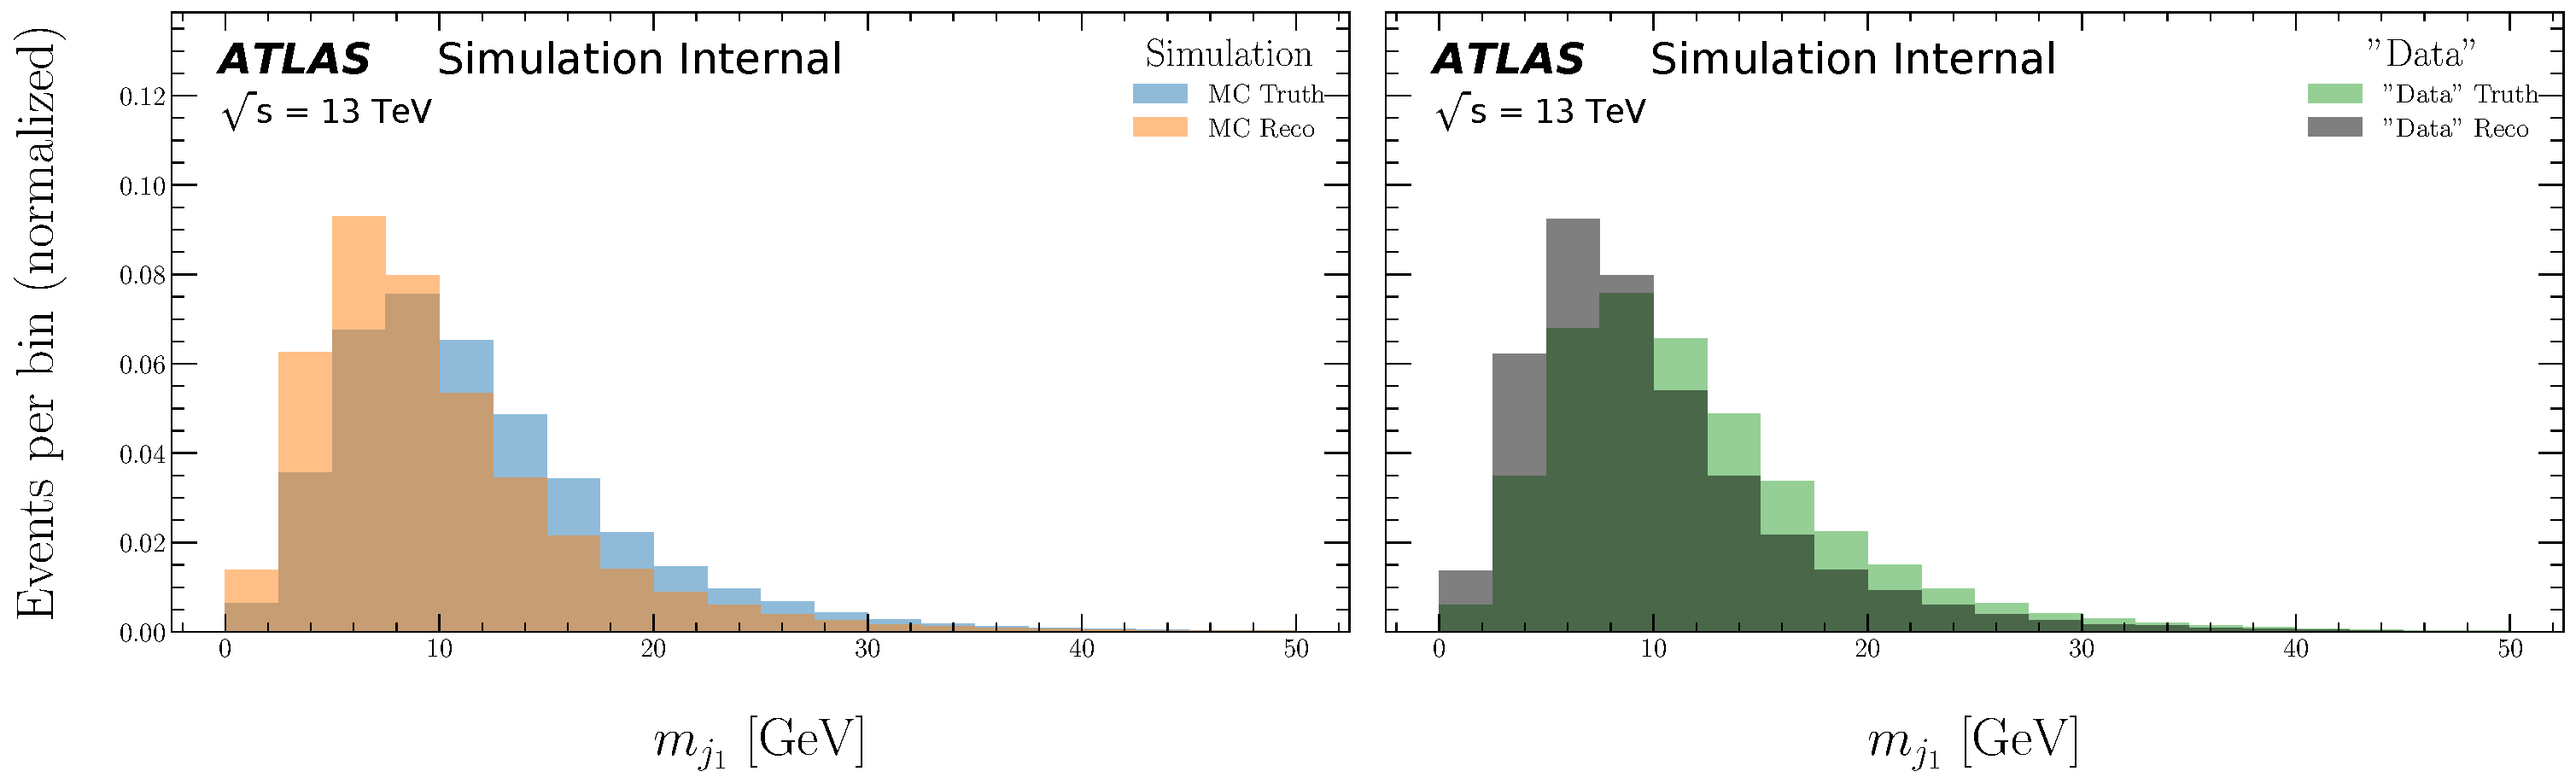
\includegraphics[width=0.95\textwidth]{figures/ATLASOmniFold-StressTest/ATLASOmniFold-TechnicalClosureTest/UniFold/m_trackj1/ATLASOmniFold-TechnicalClosureTest-UniFold-m_trackj1-Distributions.pdf}}\\
\subfloat[After 1 iteration]{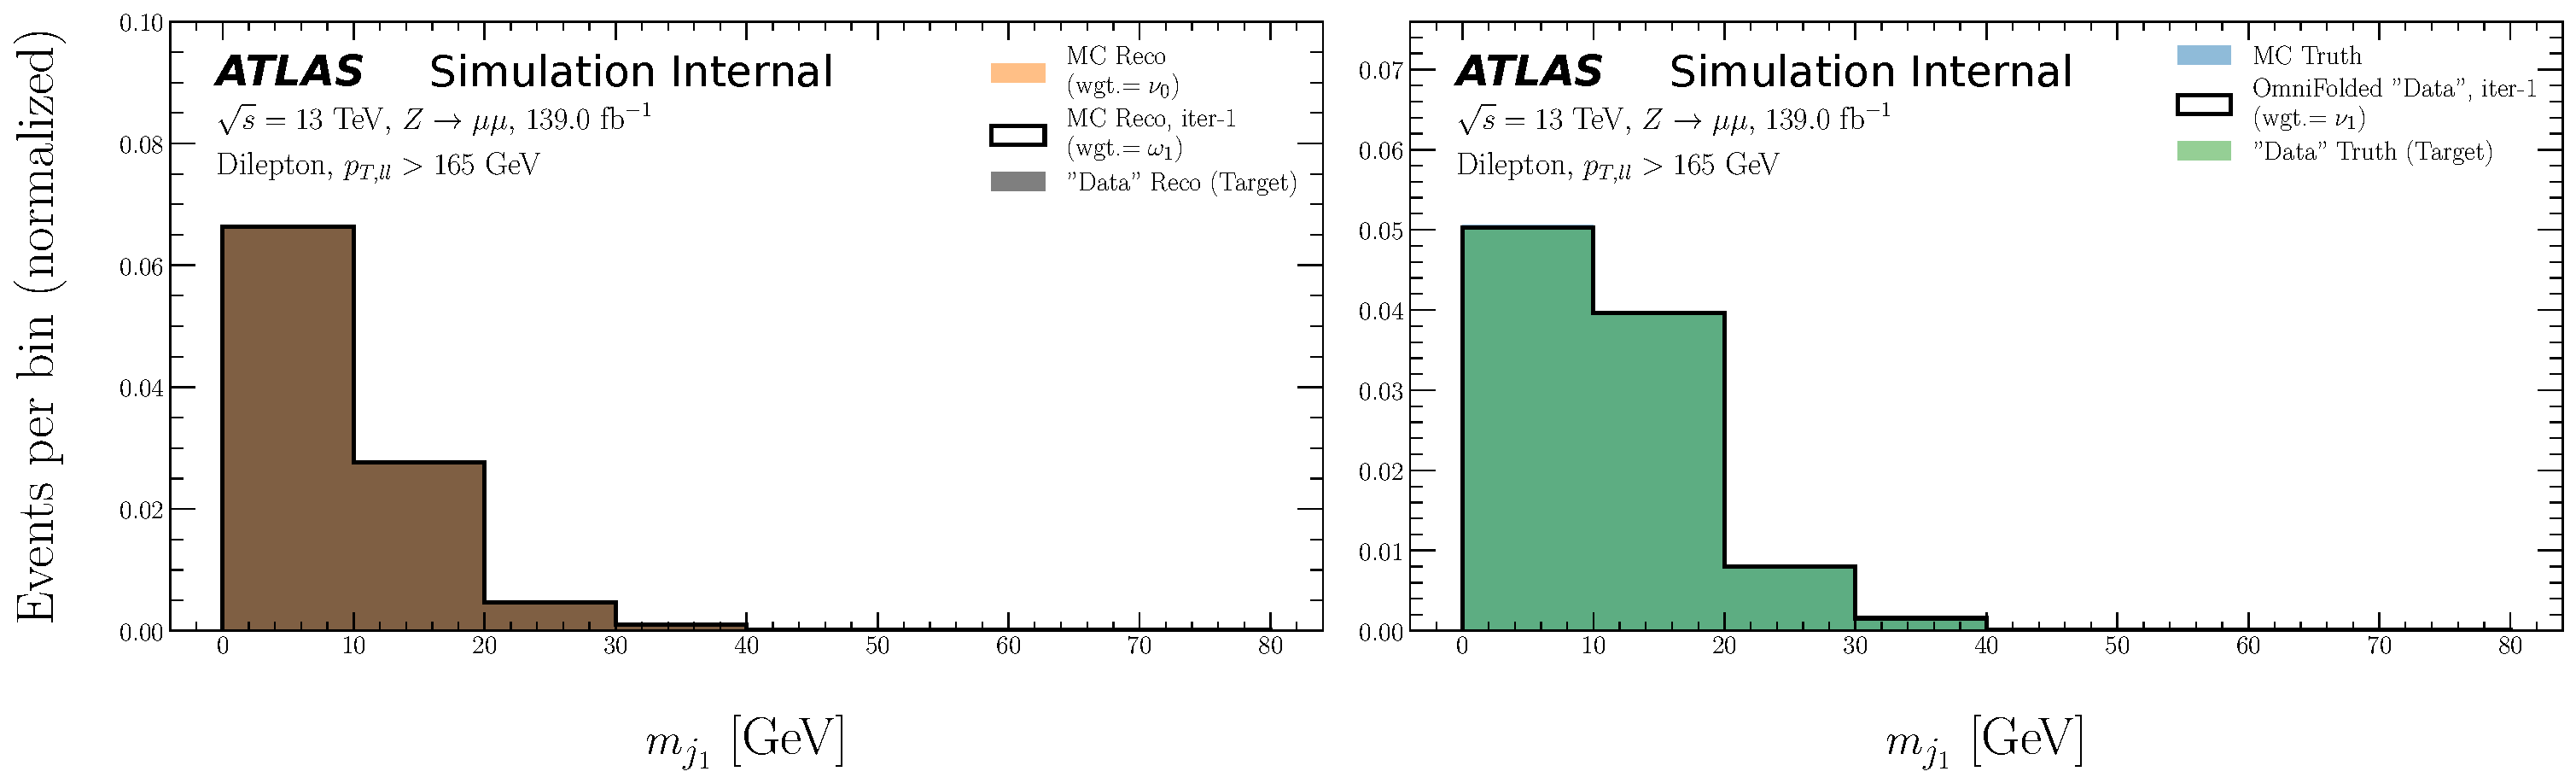
\includegraphics[width=0.95\textwidth]{figures/ATLASOmniFold-StressTest/ATLASOmniFold-TechnicalClosureTest/UniFold/m_trackj1/ATLASOmniFold-TechnicalClosureTest-UniFold-m_trackj1-Iteration01.pdf}}
\caption{A technical closure test for the mass of the leading track jet using using UniFold.  The top plot show the input histograms and the bottom plots are the results after one iteration of OmniFold.  By construction the top left and top right histograms are statistically identical.}
\label{fig:technicalclosure:mass}
\end{figure}

\begin{figure}[h!]
\centering
\subfloat[Input histograms]{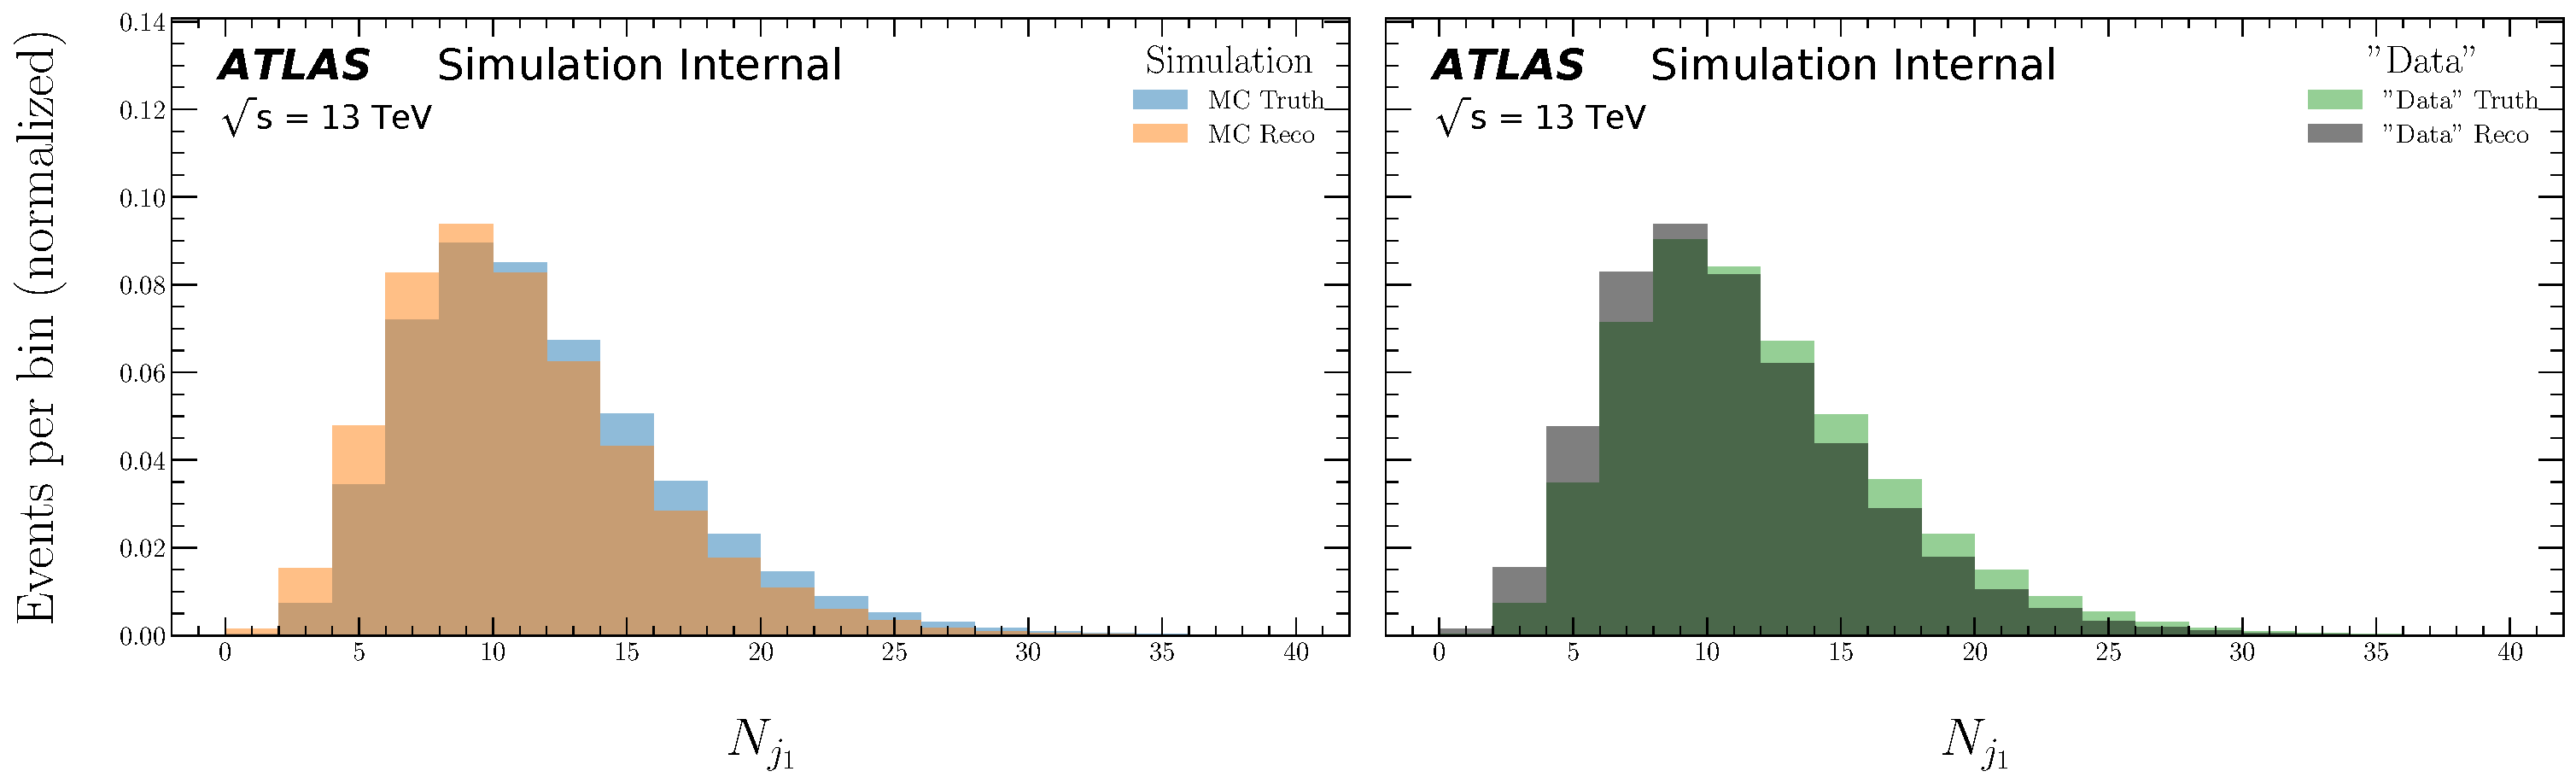
\includegraphics[width=0.95\textwidth]{figures/ATLASOmniFold-StressTest/ATLASOmniFold-TechnicalClosureTest/UniFold/Ntracks_trackj1/ATLASOmniFold-TechnicalClosureTest-UniFold-Ntracks_trackj1-Distributions.pdf}}\\
\subfloat[After 1 iteration]{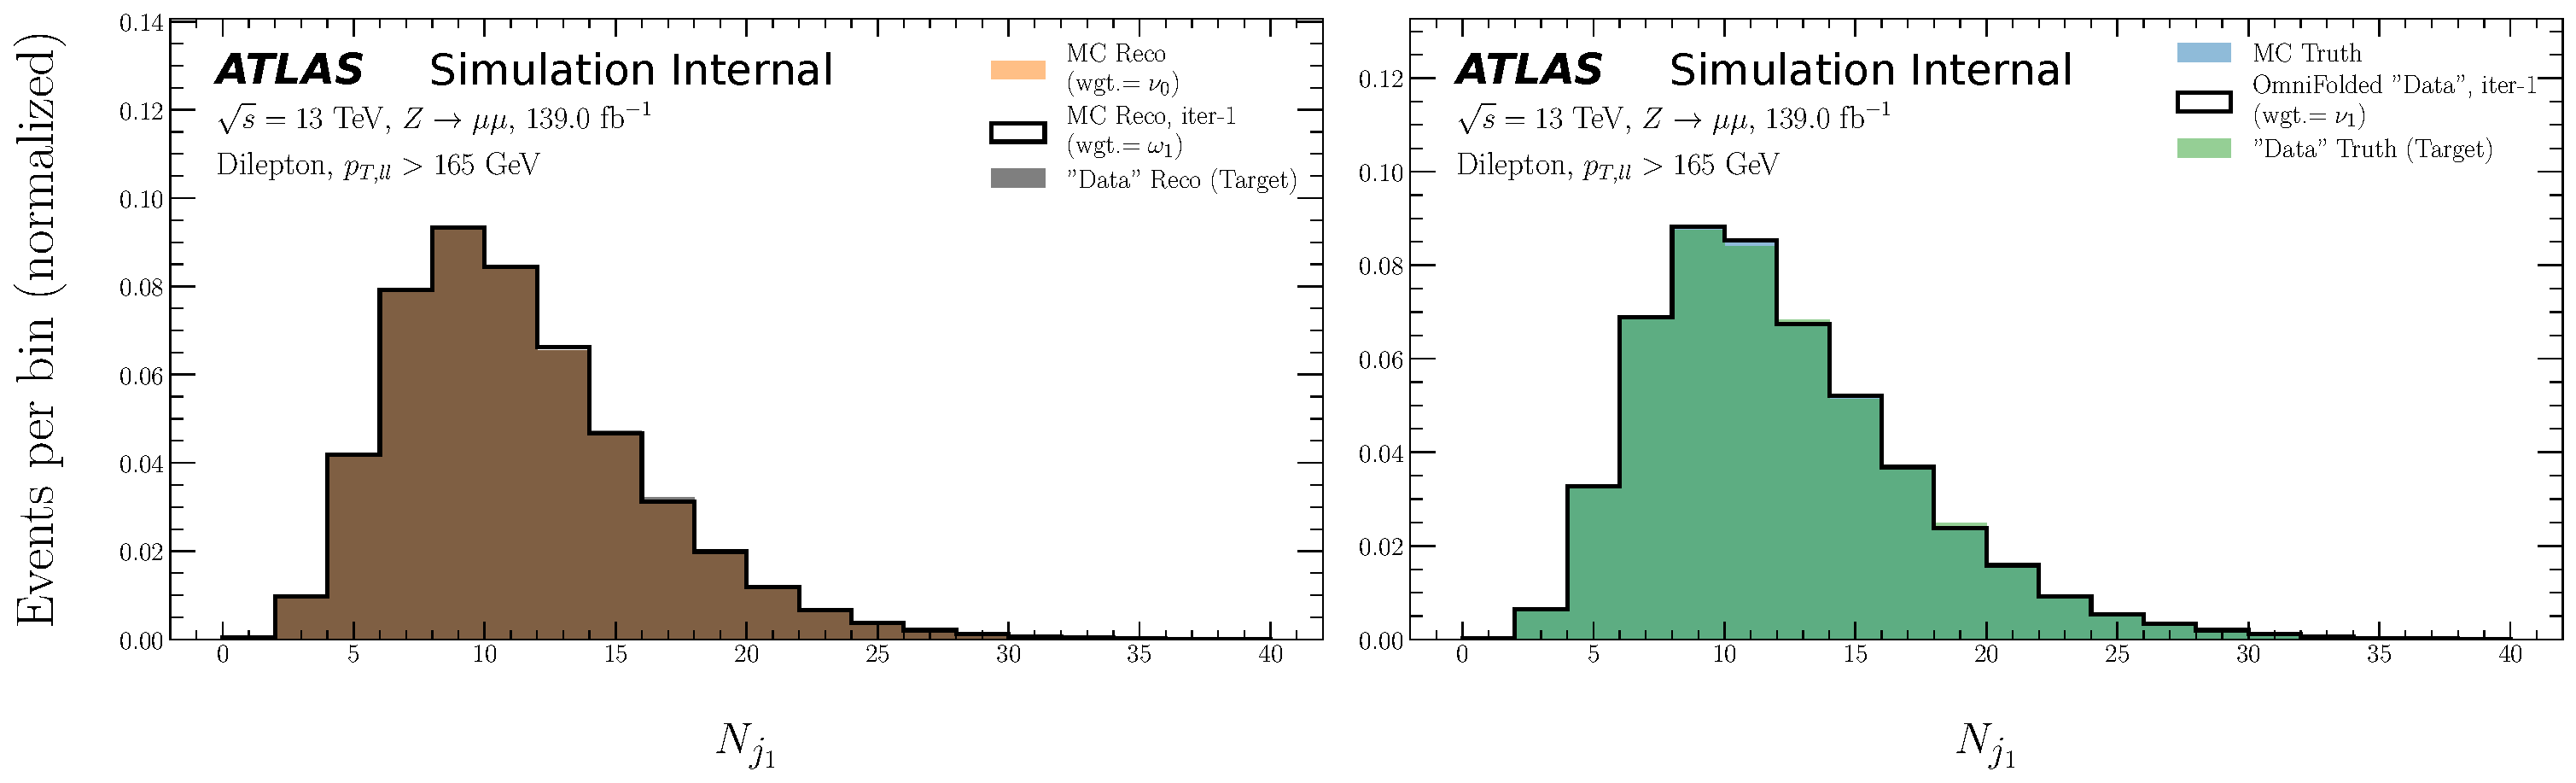
\includegraphics[width=0.95\textwidth]{figures/ATLASOmniFold-StressTest/ATLASOmniFold-TechnicalClosureTest/UniFold/Ntracks_trackj1/ATLASOmniFold-TechnicalClosureTest-UniFold-Ntracks_trackj1-Iteration01.pdf}}
\caption{A technical closure test for the number of tracks in the leading track jet using UniFold.  The top plot show the input histograms and the bottom plots are the results after one iteration of OmniFold.  By construction the top left and top right histograms are statistically identical.}
\label{fig:technicalclosure:ntracksjet1}
\end{figure}

\begin{figure}[h!]
\centering
\subfloat[Input histograms]{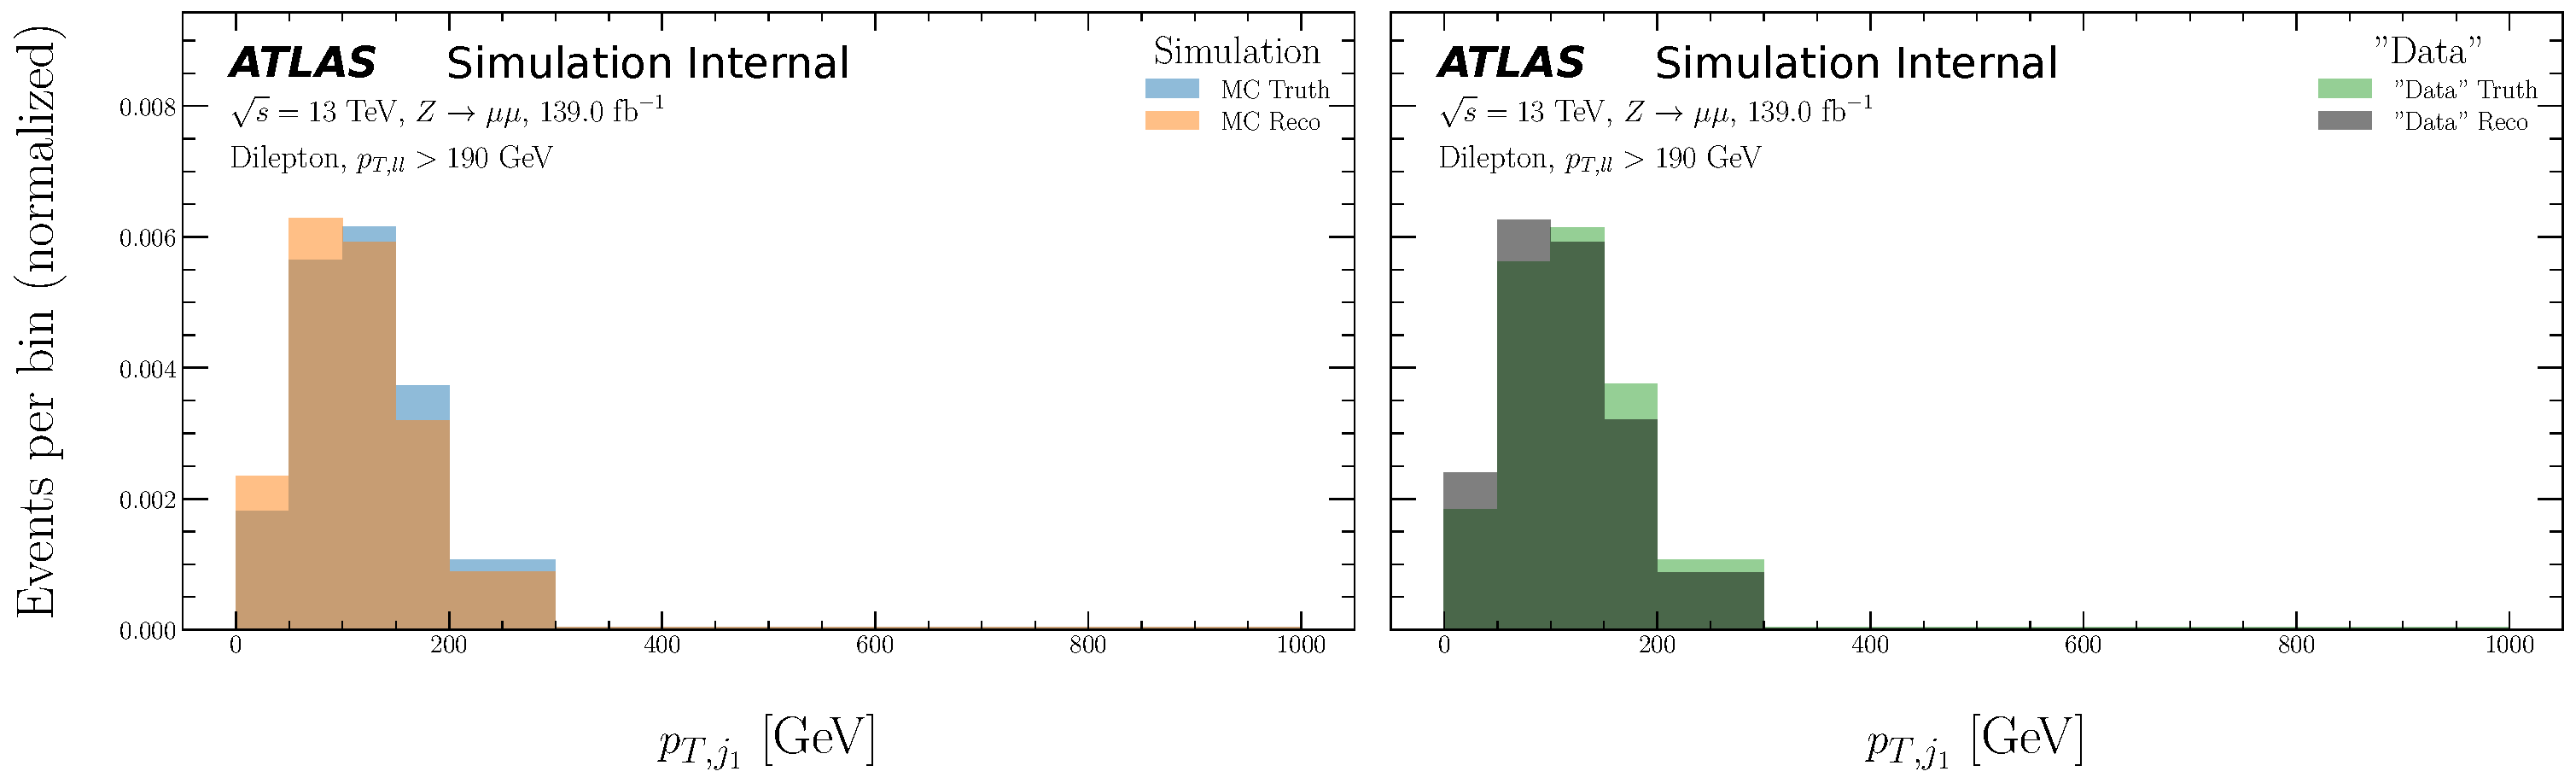
\includegraphics[width=0.95\textwidth]{figures/ATLASOmniFold-StressTest/ATLASOmniFold-TechnicalClosureTest/UniFold/pT_trackj1/ATLASOmniFold-TechnicalClosureTest-UniFold-pT_trackj1-Distributions.pdf}}\\
\subfloat[After 1 iteration]{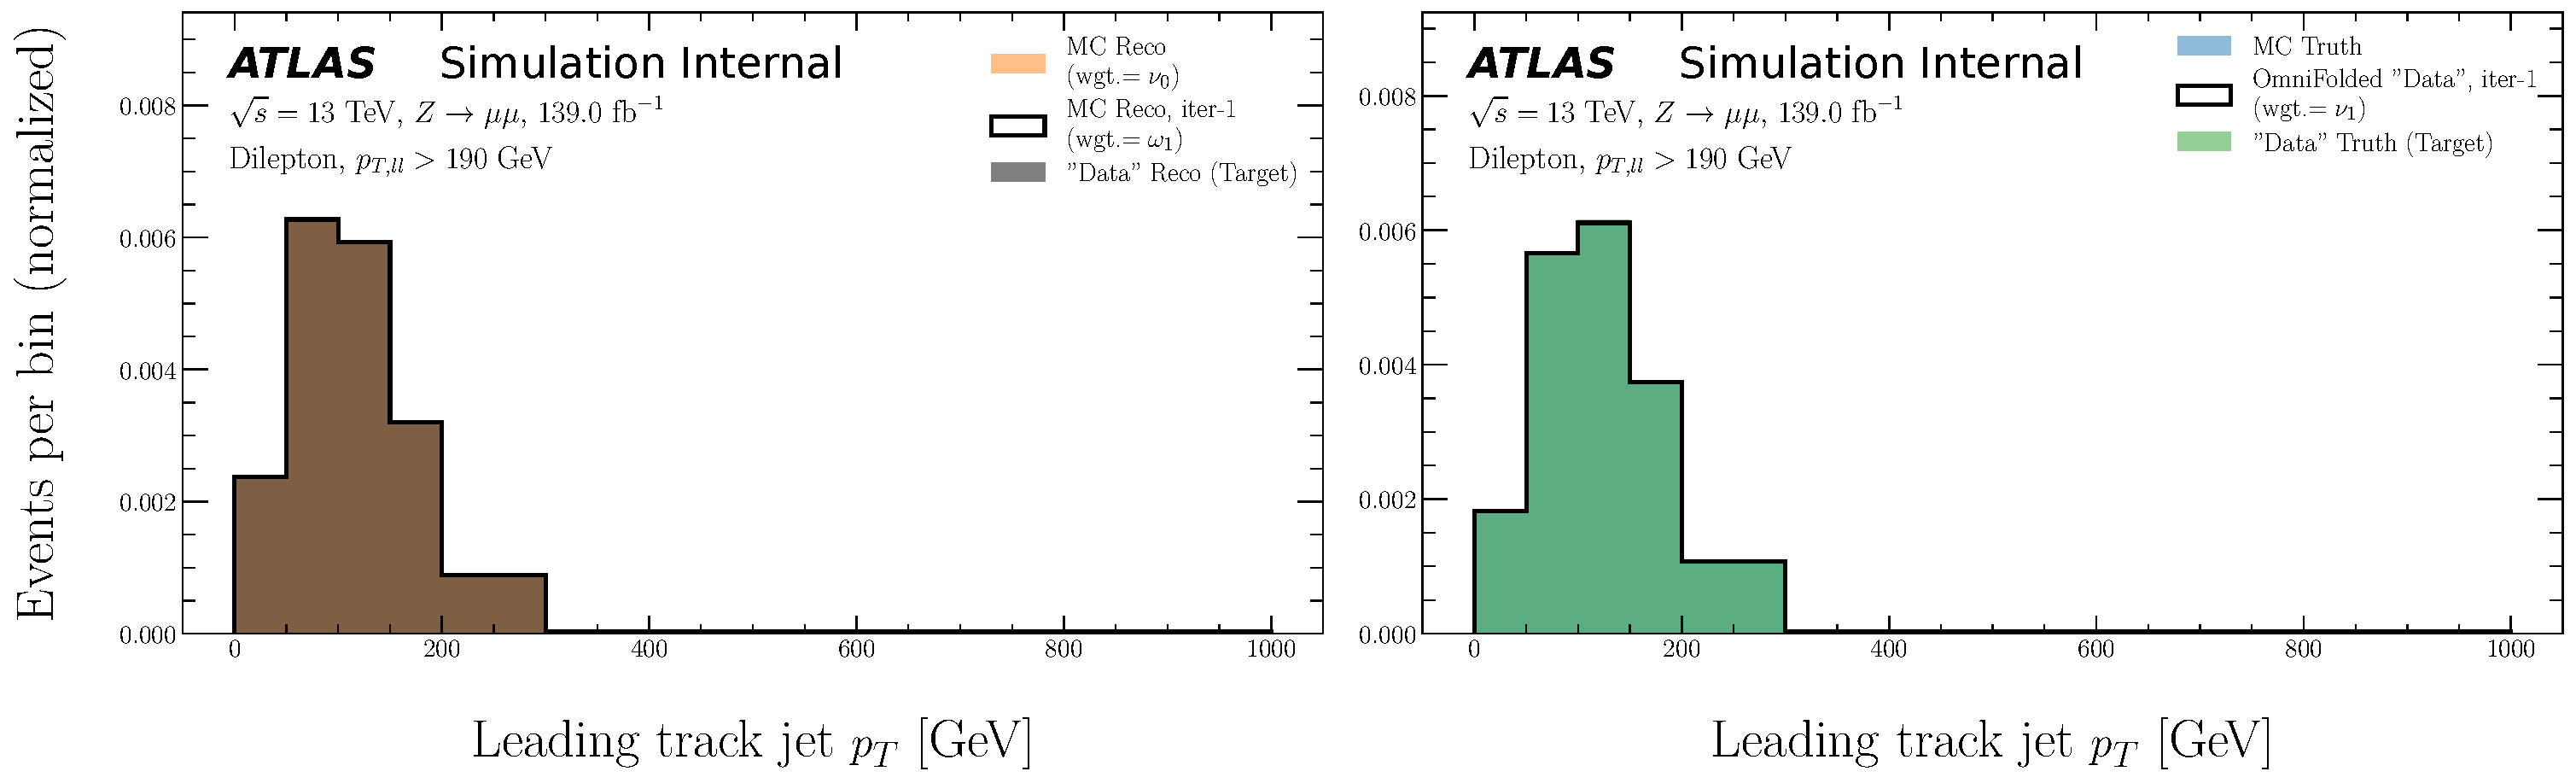
\includegraphics[width=0.95\textwidth]{figures/ATLASOmniFold-StressTest/ATLASOmniFold-TechnicalClosureTest/UniFold/pT_trackj1/ATLASOmniFold-TechnicalClosureTest-UniFold-pT_trackj1-Iteration01.pdf}}
\caption{A technical closure test for the $p_T$ of the leading track jet using UniFold.  The top plot show the input histograms and the bottom plots are the results after one iteration of OmniFold.  By construction the top left and top right histograms are statistically identical.}
\label{fig:technicalclosure:pT_trackj1}
\end{figure}

\begin{figure}[h!]
\centering
\subfloat[Input histograms]{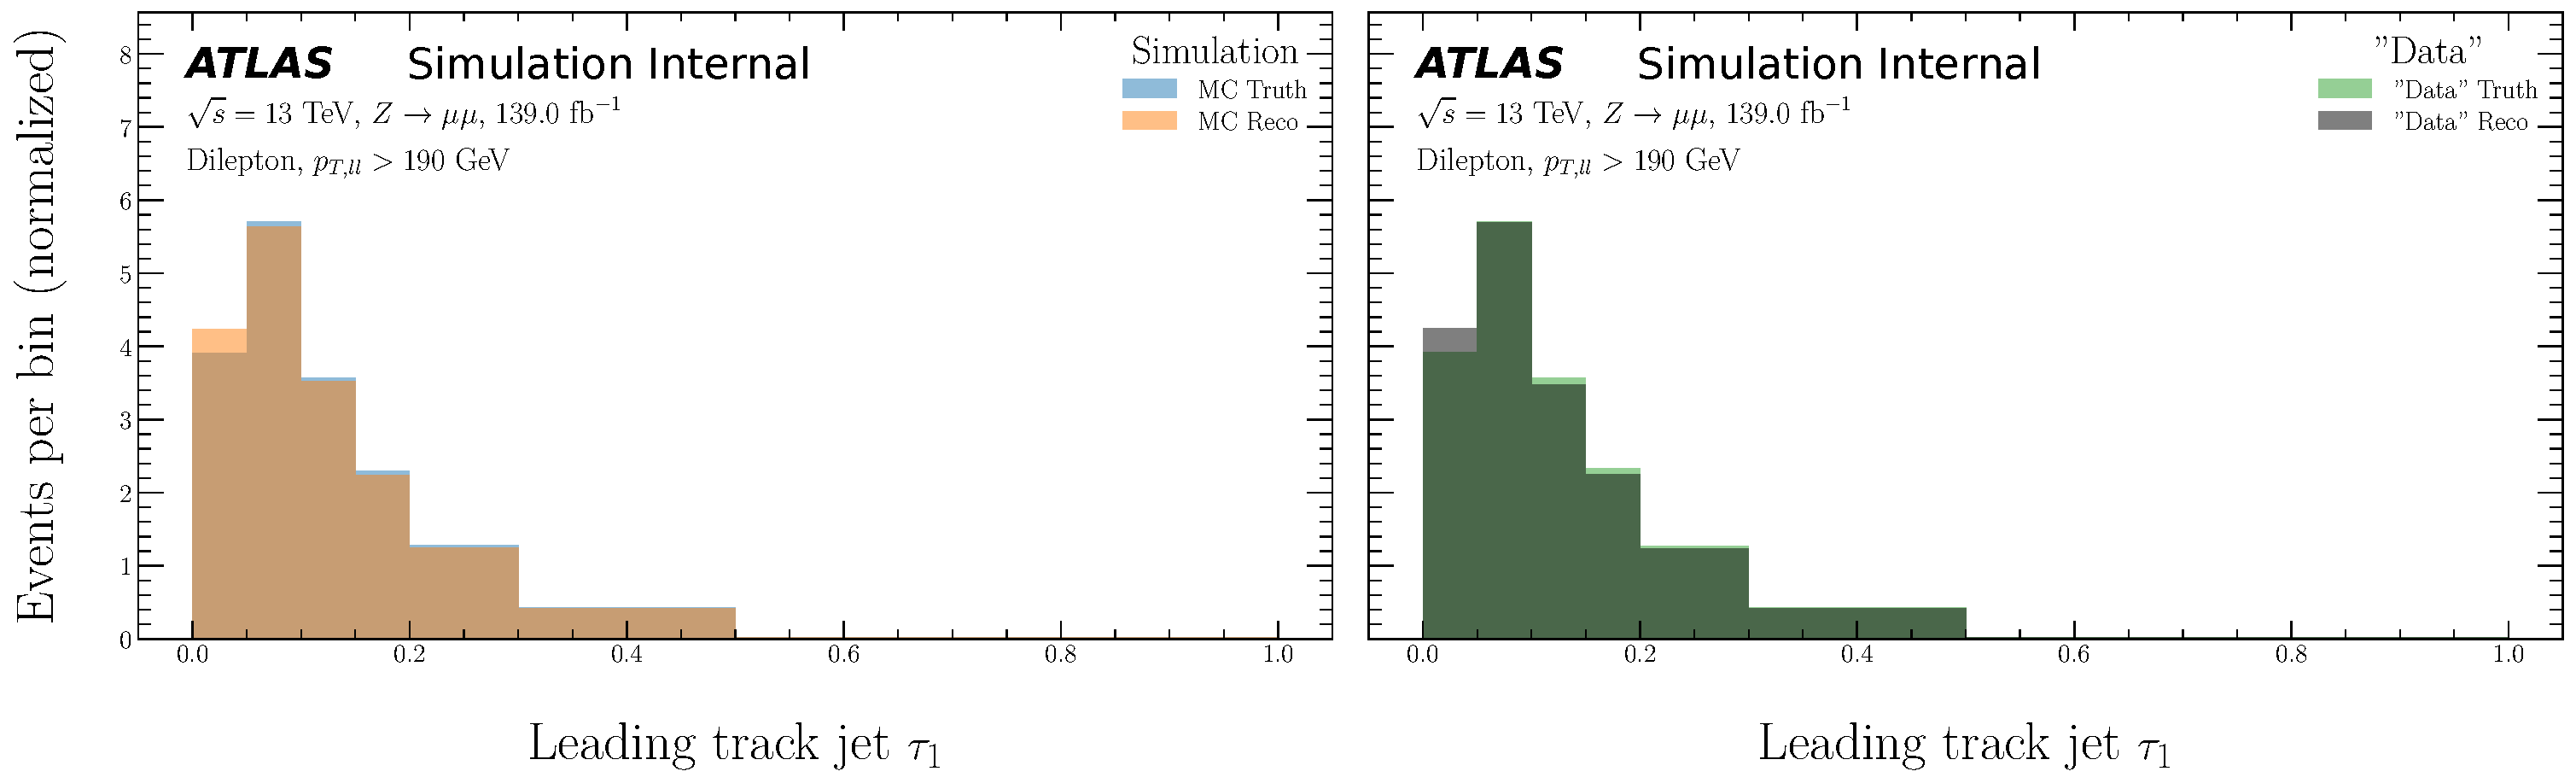
\includegraphics[width=0.89\textwidth]{figures/ATLASOmniFold-StressTest/ATLASOmniFold-TechnicalClosureTest/UniFold/tau1_trackj1/ATLASOmniFold-TechnicalClosureTest-UniFold-tau1_trackj1-Distributions.pdf}}\\
\subfloat[After 1 iteration]{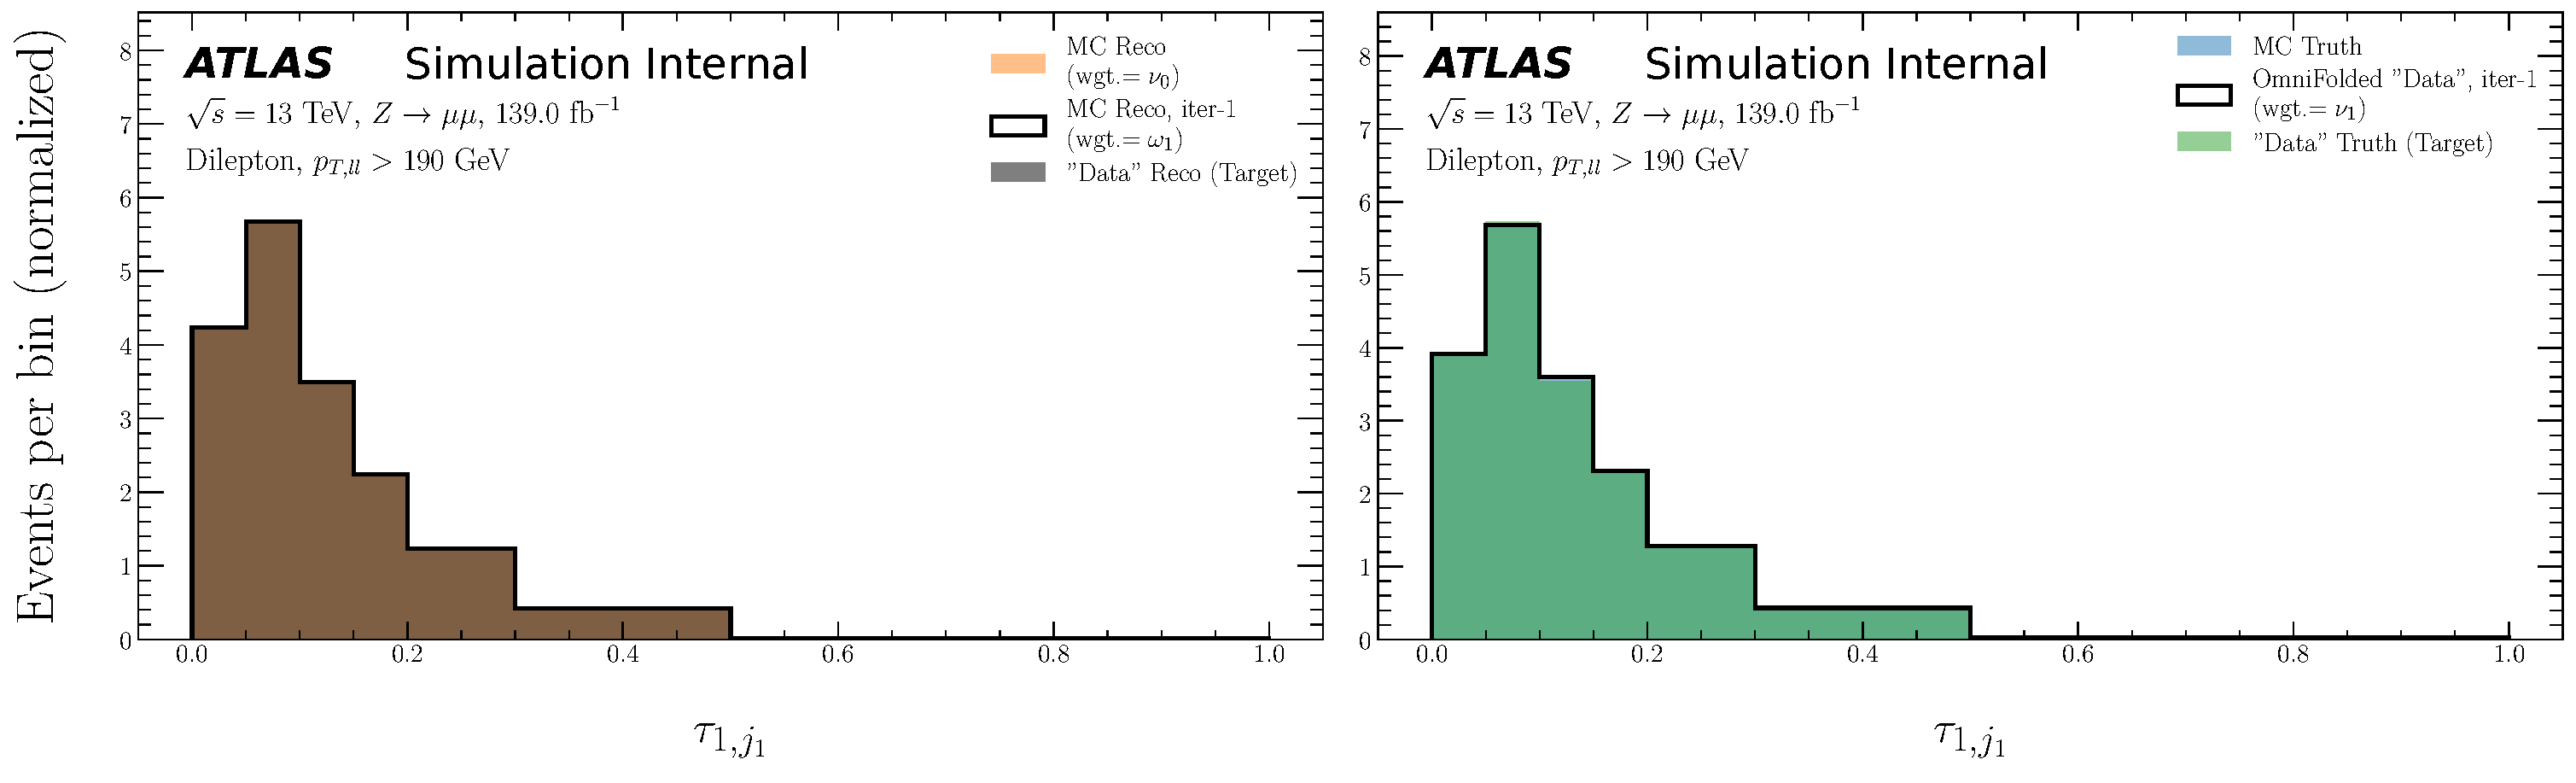
\includegraphics[width=0.95\textwidth]{figures/ATLASOmniFold-StressTest/ATLASOmniFold-TechnicalClosureTest/UniFold/tau1_trackj1/ATLASOmniFold-TechnicalClosureTest-UniFold-tau1_trackj1-Iteration01.pdf}}
\caption{A technical closure test for the $\tau_1$ of the leading track jet using UniFold.  The top plot show the input histograms and the bottom plots are the results after one iteration of OmniFold.  By construction the top left and top right histograms are statistically identical.}
\label{fig:technicalclosure:tau1_trackj1}
\end{figure}

\begin{figure}[h!]
\centering
\subfloat[Input histograms]{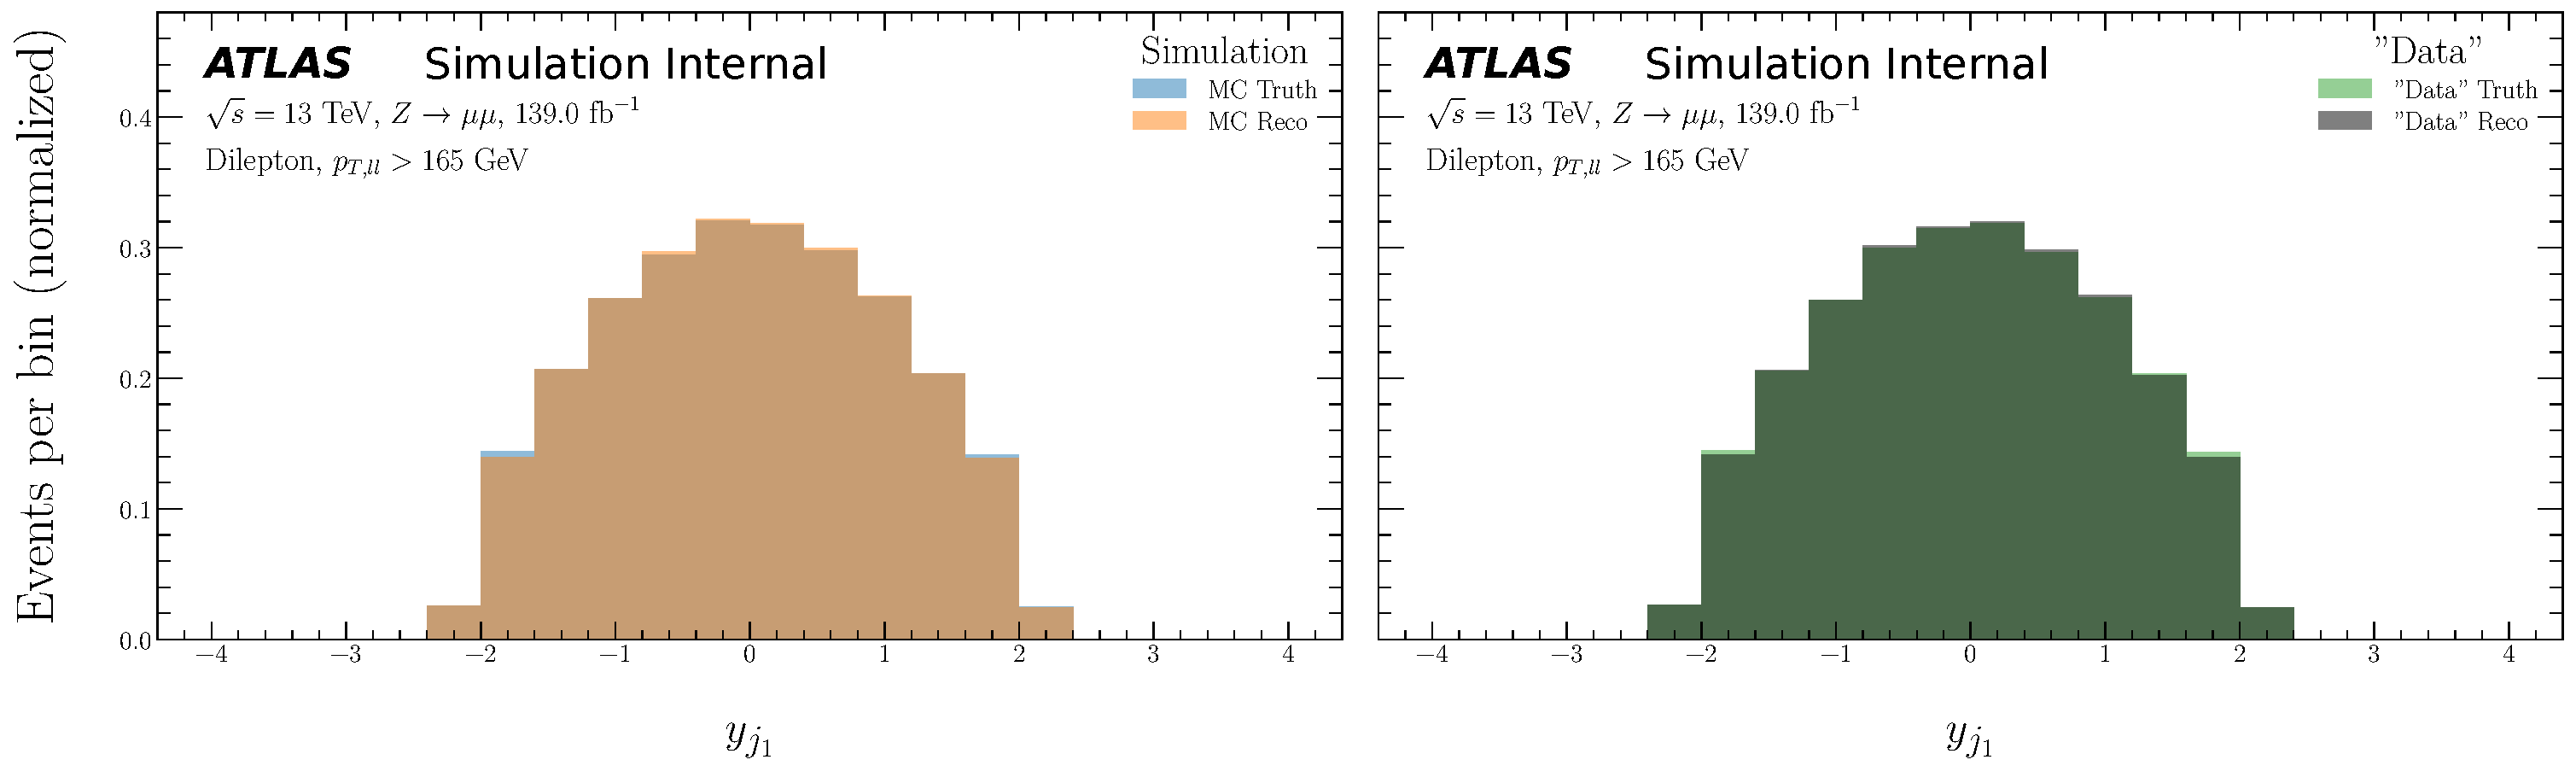
\includegraphics[width=0.95\textwidth]{figures/ATLASOmniFold-StressTest/ATLASOmniFold-TechnicalClosureTest/UniFold/y_trackj1/ATLASOmniFold-TechnicalClosureTest-UniFold-y_trackj1-Distributions.pdf}}\\
\subfloat[After 1 iteration]{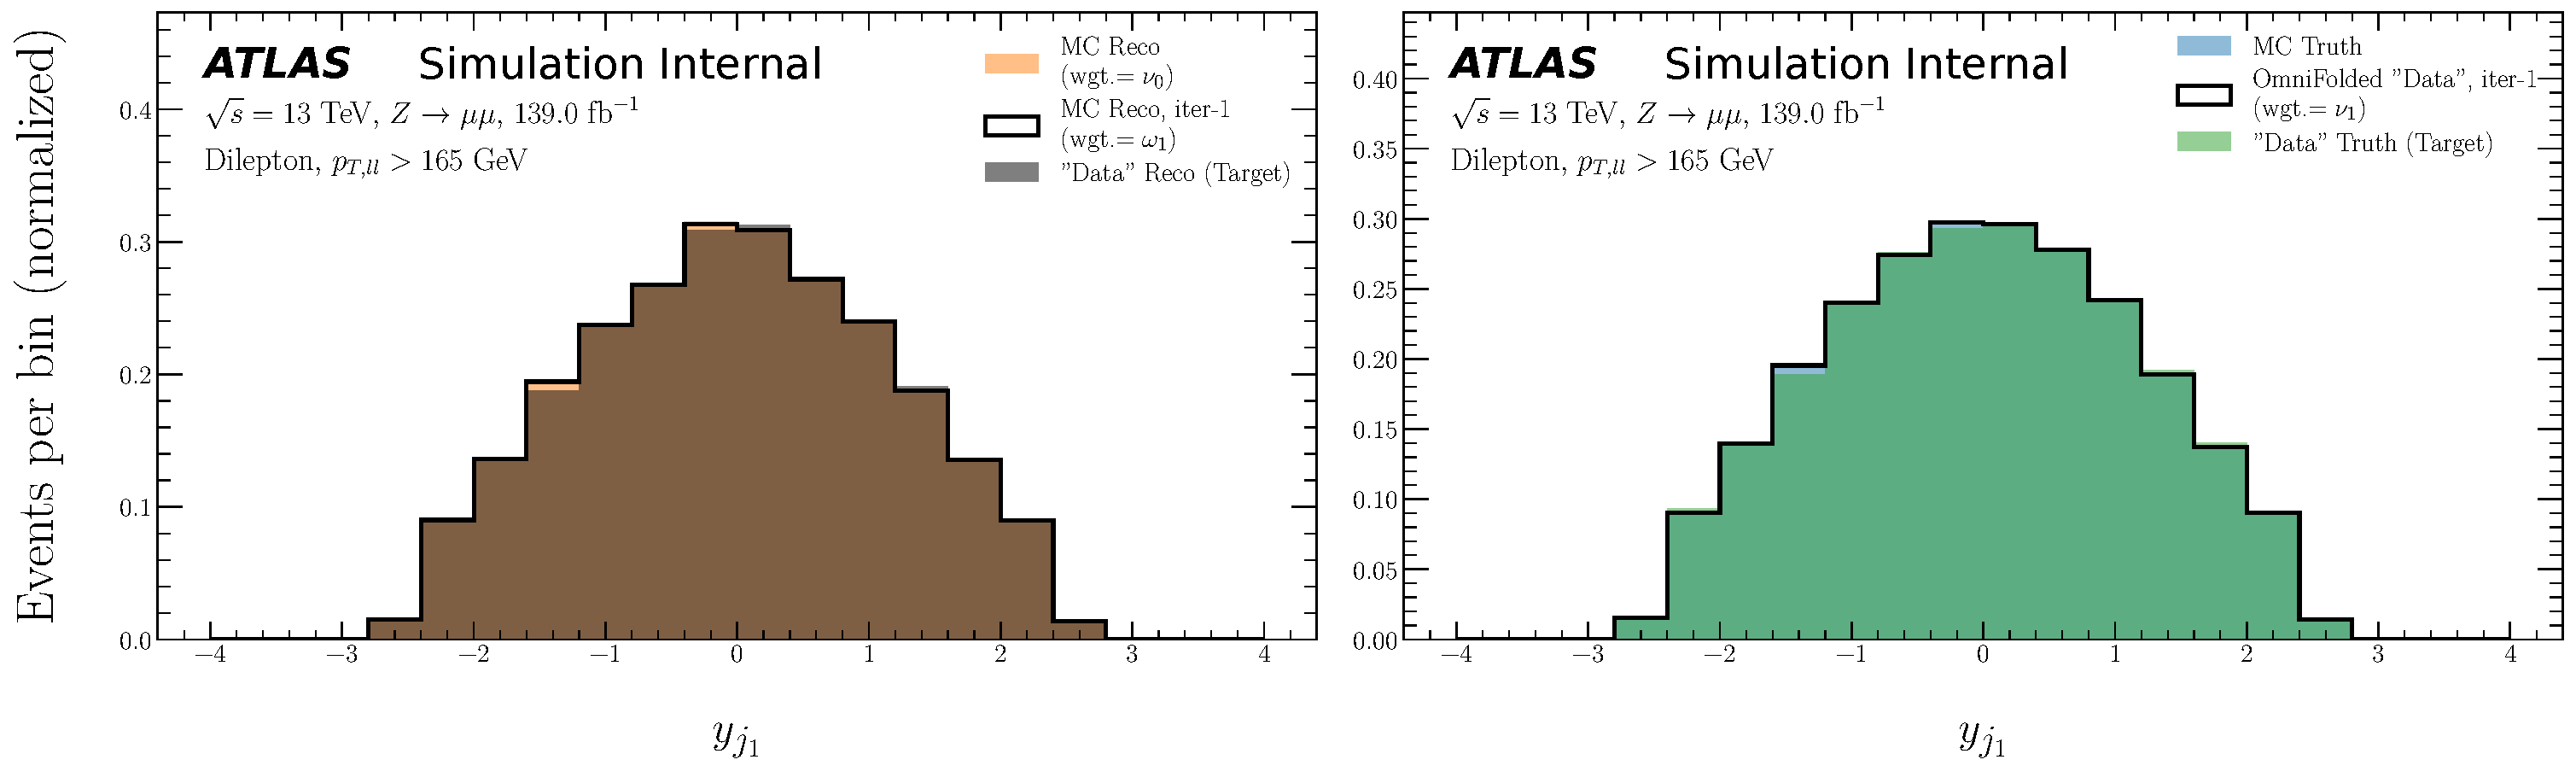
\includegraphics[width=0.95\textwidth]{figures/ATLASOmniFold-StressTest/ATLASOmniFold-TechnicalClosureTest/UniFold/y_trackj1/ATLASOmniFold-TechnicalClosureTest-UniFold-y_trackj1-Iteration01.pdf}}
\caption{A technical closure test for the rapidity of the leading track jet using UniFold.  The top plot show the input histograms and the bottom plots are the results after one iteration of OmniFold.  By construction the top left and top right histograms are statistically identical.}
\label{fig:technicalclosure:y_trackj1}
\end{figure}

\subsubsection{MultiFold}
\label{sec:technicalclosure:multifold}

In this section, we determine the closure of a 16-dimensional unfolding that includes $y_{\mu^+\mu^-},p_{T,\mu^+\mu^-}$ and the following properties of the leading and subleading track jets: mass, constituent multiplicity, $p_T$, rapidity, $\phi$, $\tau_1$, $\tau_2$, and $\tau_3$.  For illustration, the same five observables as in Sec.~\ref{sec:technicalclosure:unifold} are shown in figures~\ref{fig:technicalclosureMulti:mass},~\ref{fig:technicalclosureMulti:ntracksjet1},~\ref{fig:technicalclosureMulti:pT_trackj1},~\ref{fig:technicalclosureMulti:tau1_trackj1}, and~\ref{fig:technicalclosureMulti:y_trackj1}, but the quality of the technical closure is excellent for any projection of the 16-dimensional space (the remaining 11 observables histograms are in App.~\ref{sec:multifoldtechnicalclosure}).

\begin{figure}[h!]
\centering
\subfloat[Input histograms]{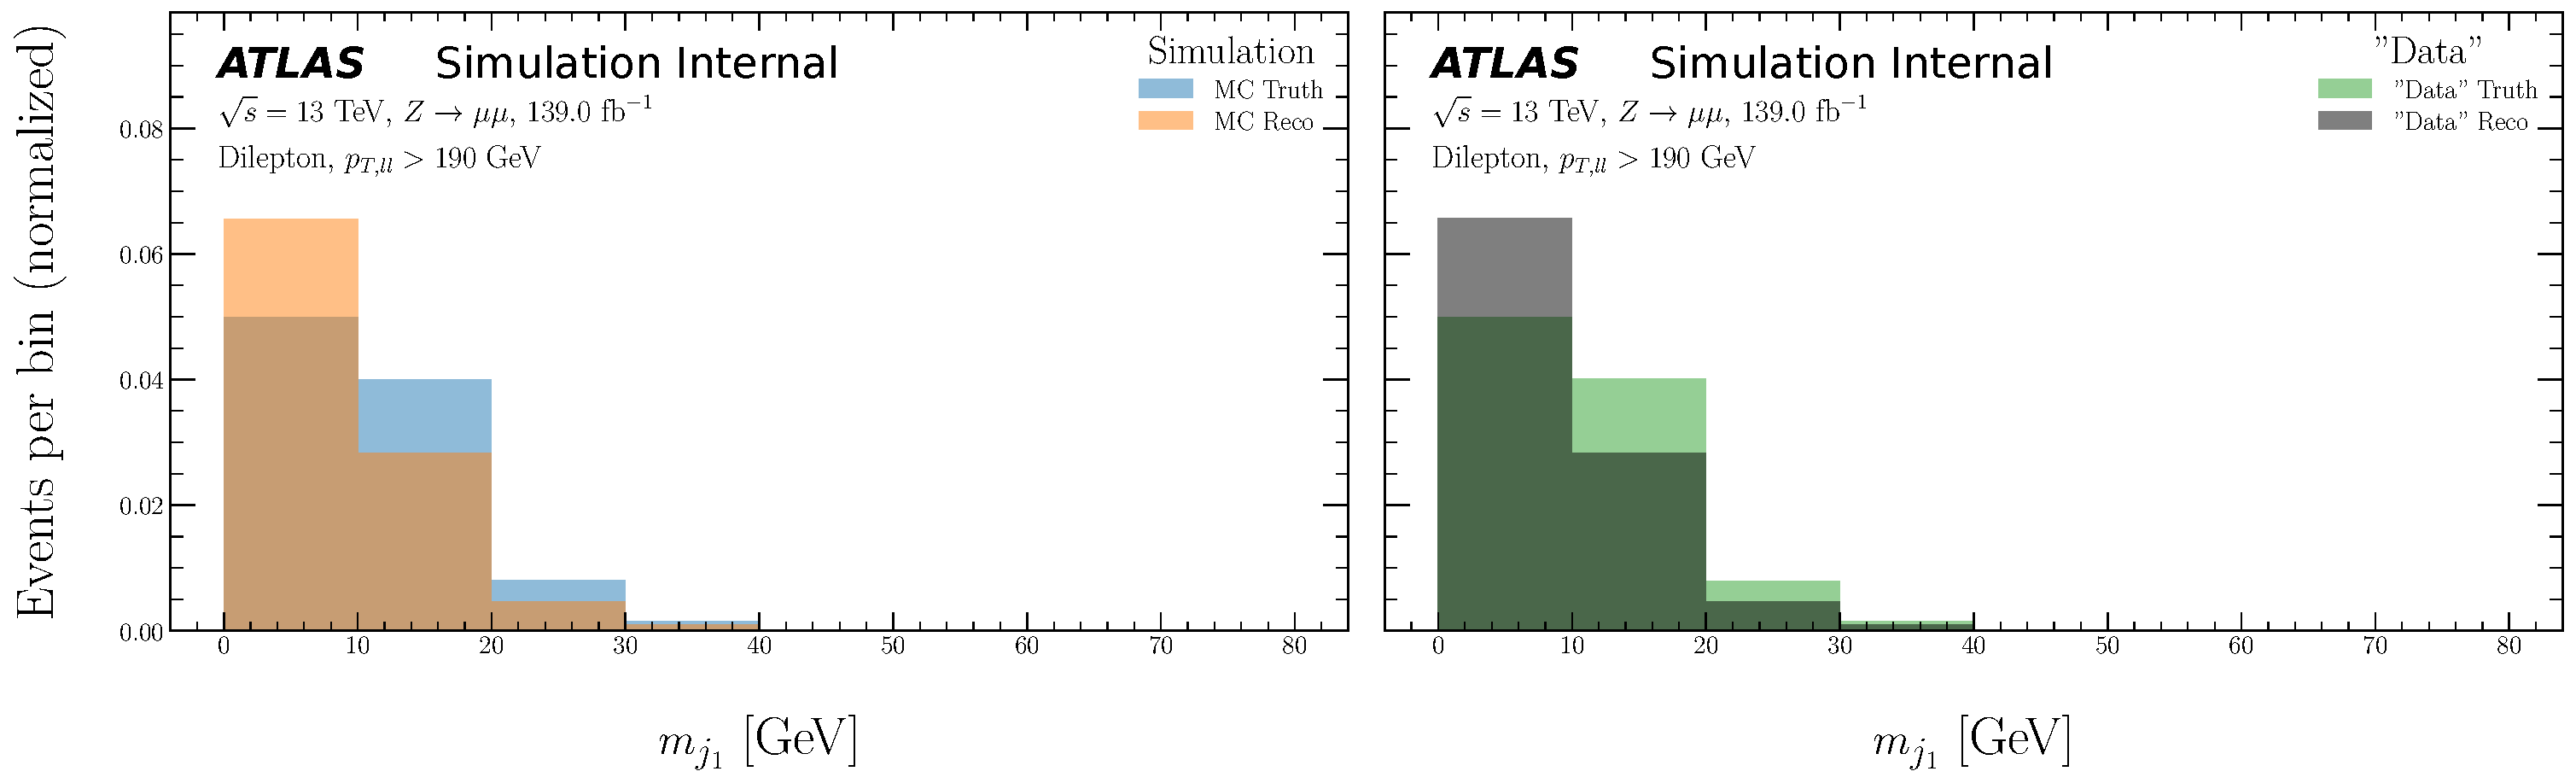
\includegraphics[width=0.95\textwidth]{figures/ATLASOmniFold-StressTest/ATLASOmniFold-TechnicalClosureTest/MultiFold/m_trackj1/ATLASOmniFold-TechnicalClosureTest-MultiFold-m_trackj1-Distributions.pdf}}\\
\subfloat[After 1 iteration]{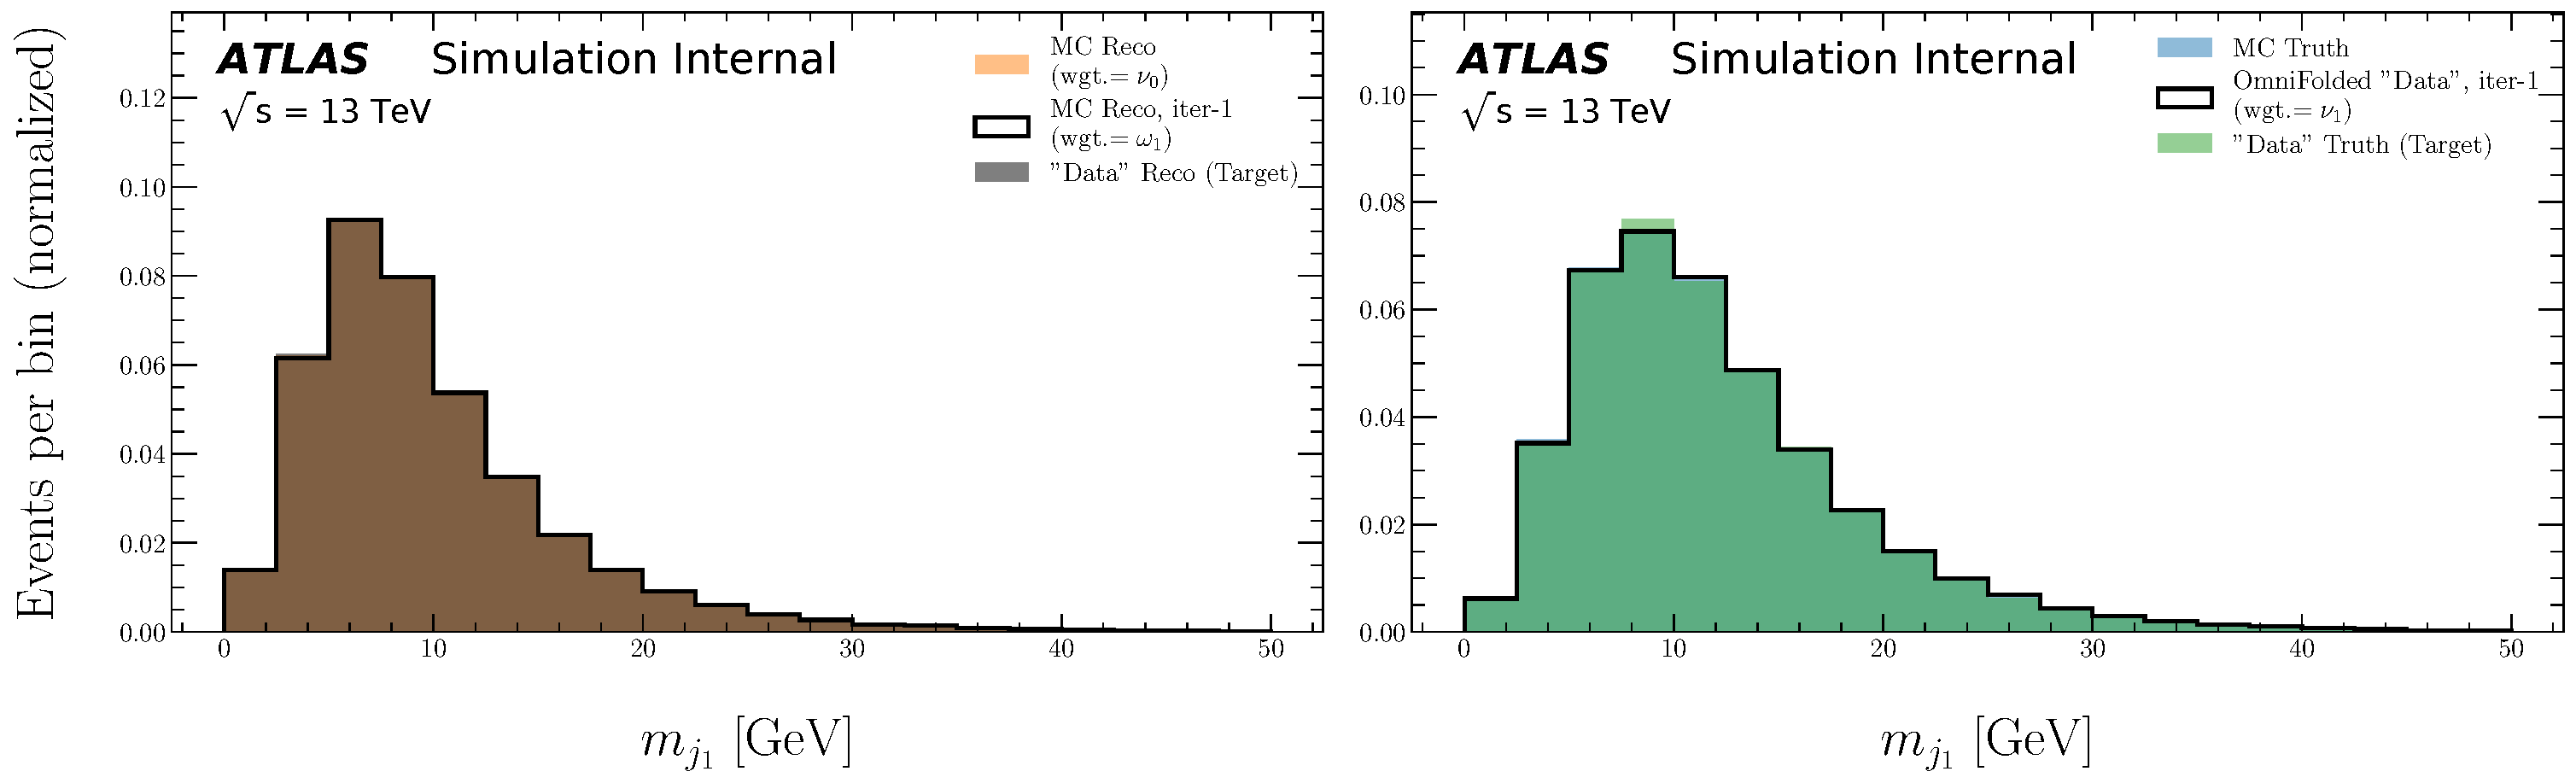
\includegraphics[width=0.95\textwidth]{figures/ATLASOmniFold-StressTest/ATLASOmniFold-TechnicalClosureTest/MultiFold/m_trackj1/ATLASOmniFold-TechnicalClosureTest-MultiFold-m_trackj1-Iteration01.pdf}}
\caption{A technical closure test for the mass of the leading track jet using using MultiFold (16 observables are simultaneously unfolded).  The top plot show the input histograms and the bottom plots are the results after one iteration of OmniFold.  By construction the top left and top right histograms are statistically identical.}
\label{fig:technicalclosureMulti:mass}
\end{figure}

\begin{figure}[h!]
\centering
\subfloat[Input histograms]{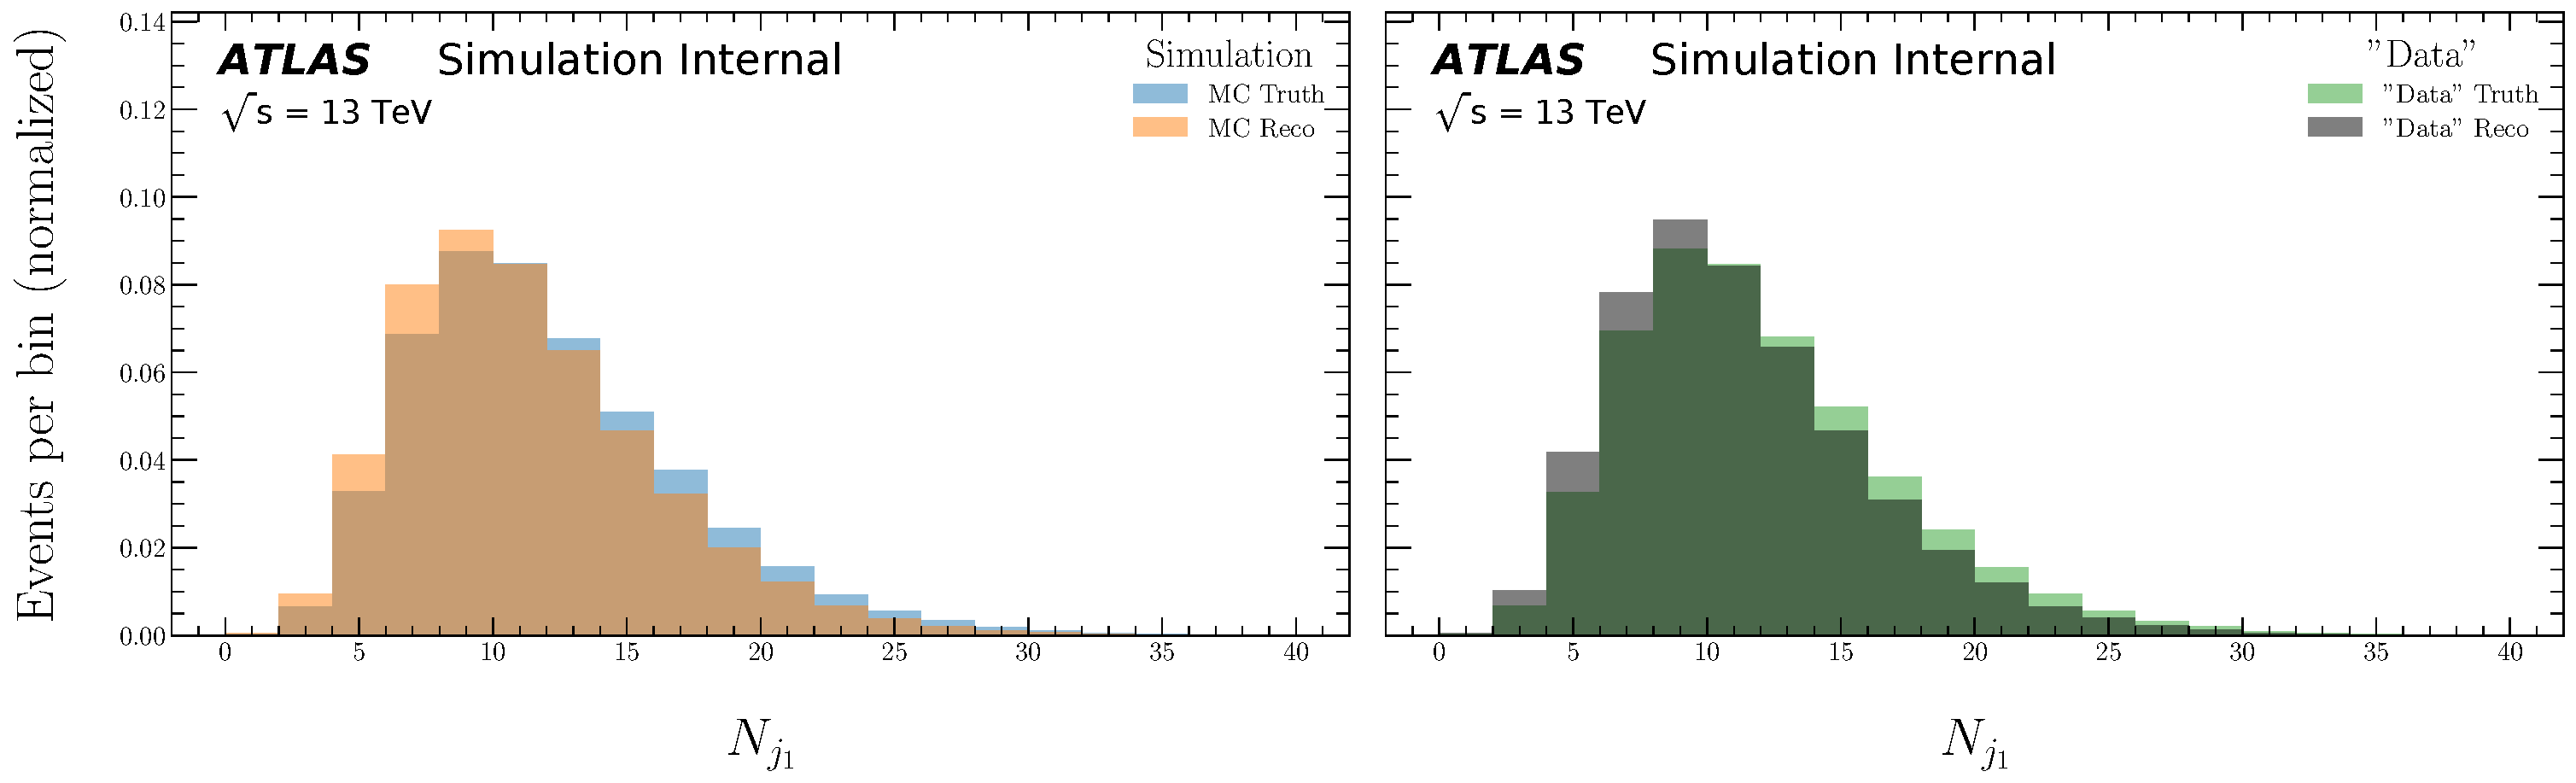
\includegraphics[width=0.95\textwidth]{figures/ATLASOmniFold-StressTest/ATLASOmniFold-TechnicalClosureTest/MultiFold/Ntracks_trackj1/ATLASOmniFold-TechnicalClosureTest-MultiFold-Ntracks_trackj1-Distributions.pdf}}\\
\subfloat[After 1 iteration]{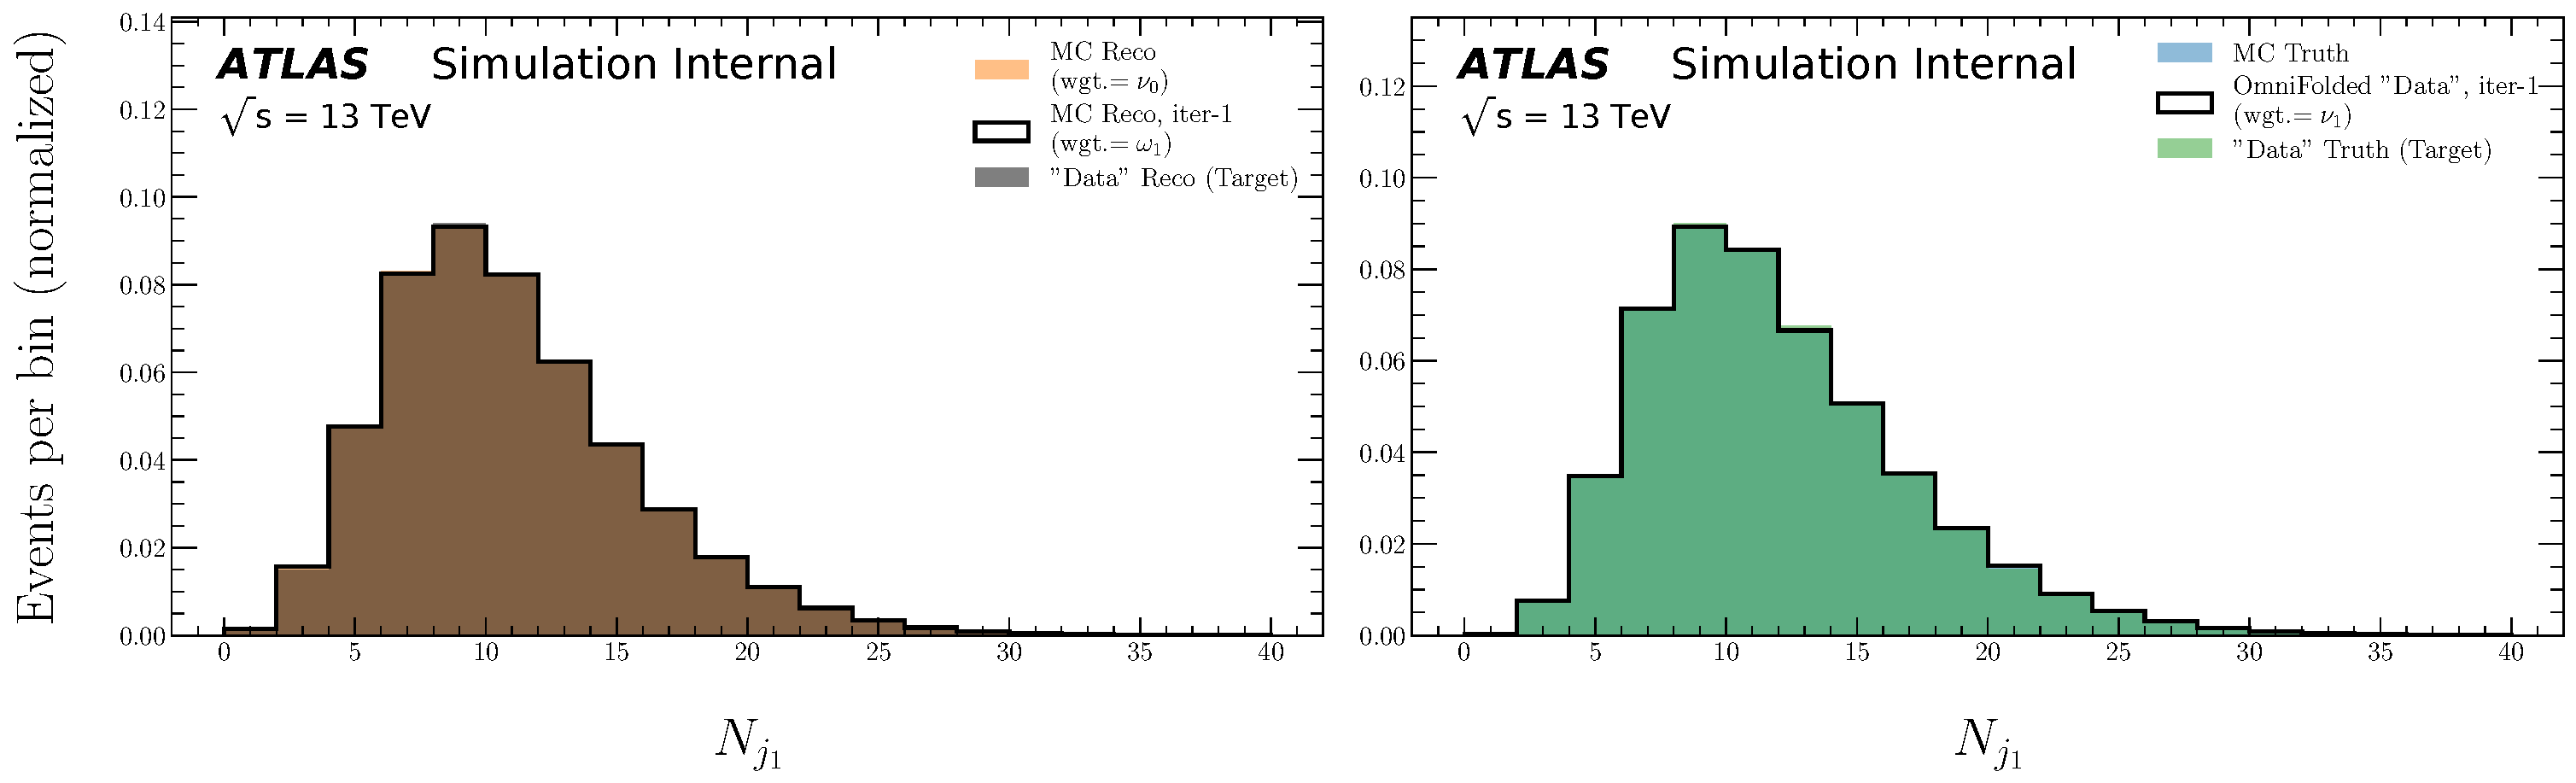
\includegraphics[width=0.95\textwidth]{figures/ATLASOmniFold-StressTest/ATLASOmniFold-TechnicalClosureTest/MultiFold/Ntracks_trackj1/ATLASOmniFold-TechnicalClosureTest-MultiFold-Ntracks_trackj1-Iteration01.pdf}}
\caption{A technical closure test for the number of tracks in the leading track jet using MultiFold (16 observables are simultaneously unfolded).  The top plot show the input histograms and the bottom plots are the results after one iteration of OmniFold.  By construction the top left and top right histograms are statistically identical.}
\label{fig:technicalclosureMulti:ntracksjet1}
\end{figure}

\begin{figure}[h!]
\centering
\subfloat[Input histograms]{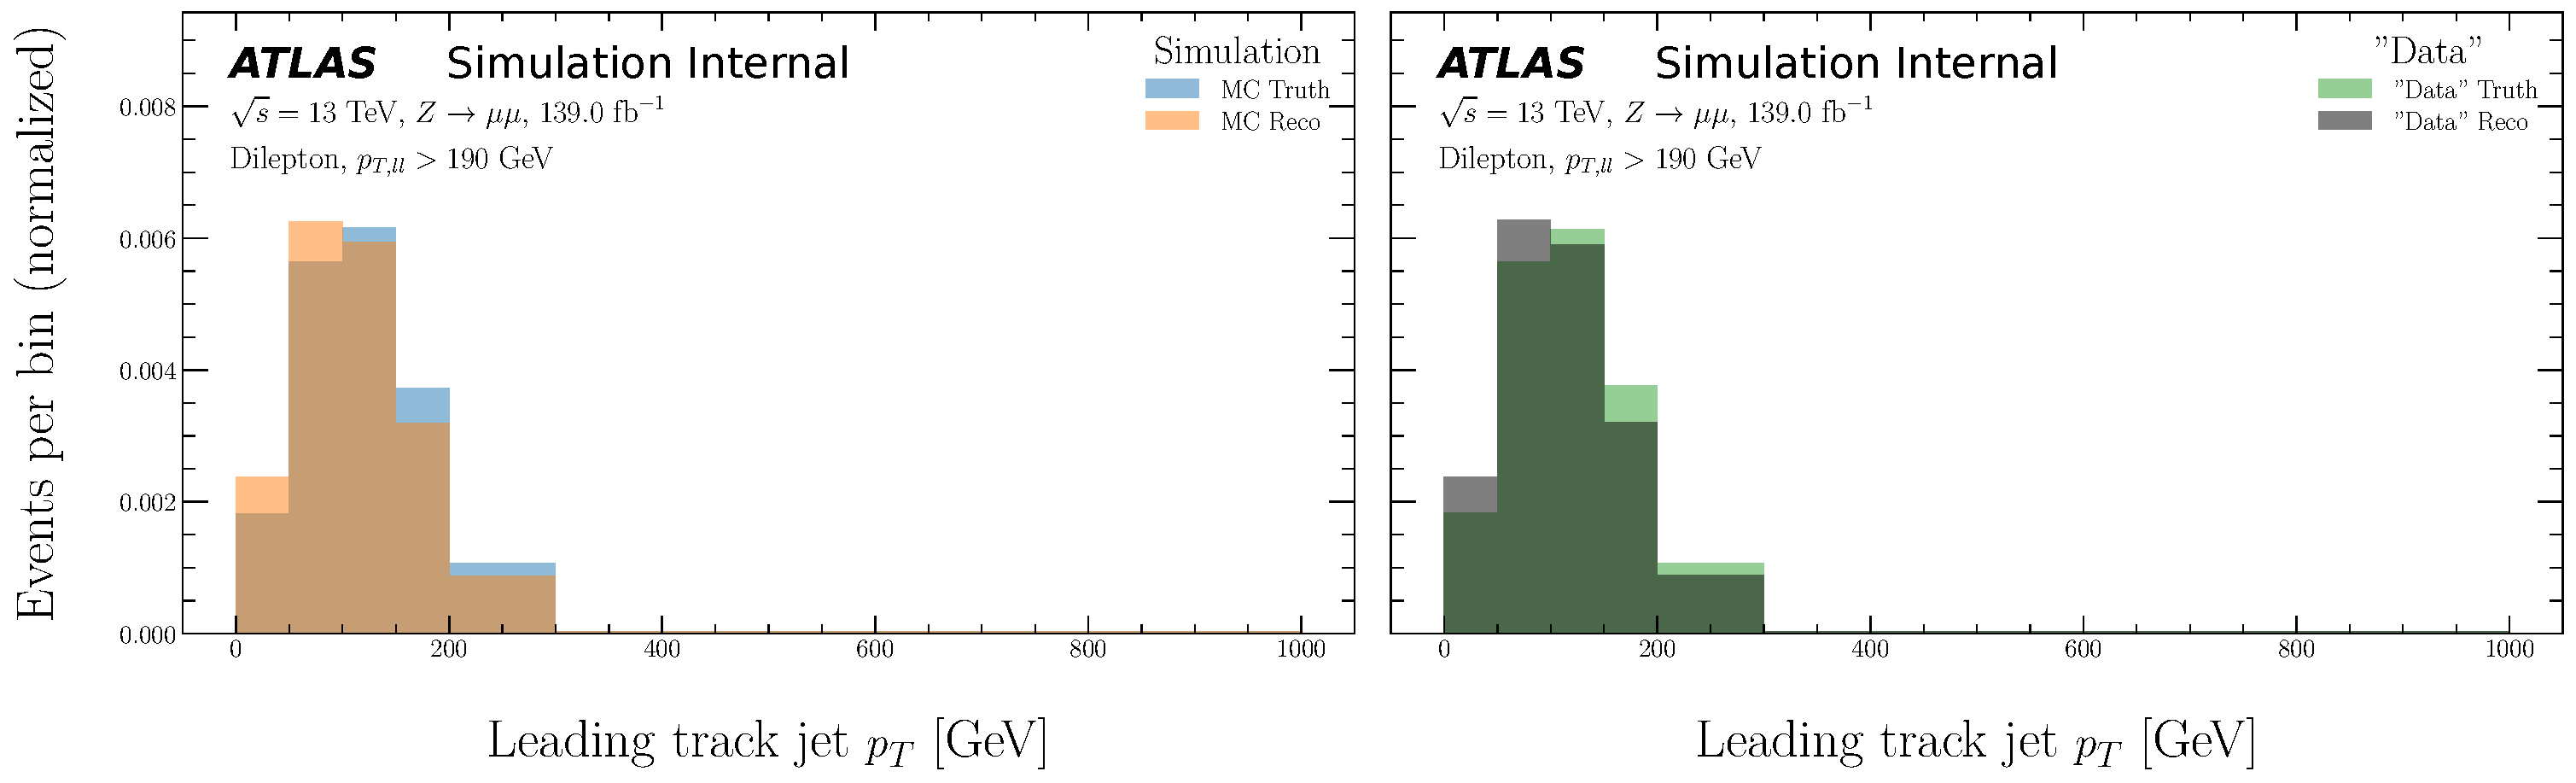
\includegraphics[width=0.95\textwidth]{figures/ATLASOmniFold-StressTest/ATLASOmniFold-TechnicalClosureTest/MultiFold/pT_trackj1/ATLASOmniFold-TechnicalClosureTest-MultiFold-pT_trackj1-Distributions.pdf}}\\
\subfloat[After 1 iteration]{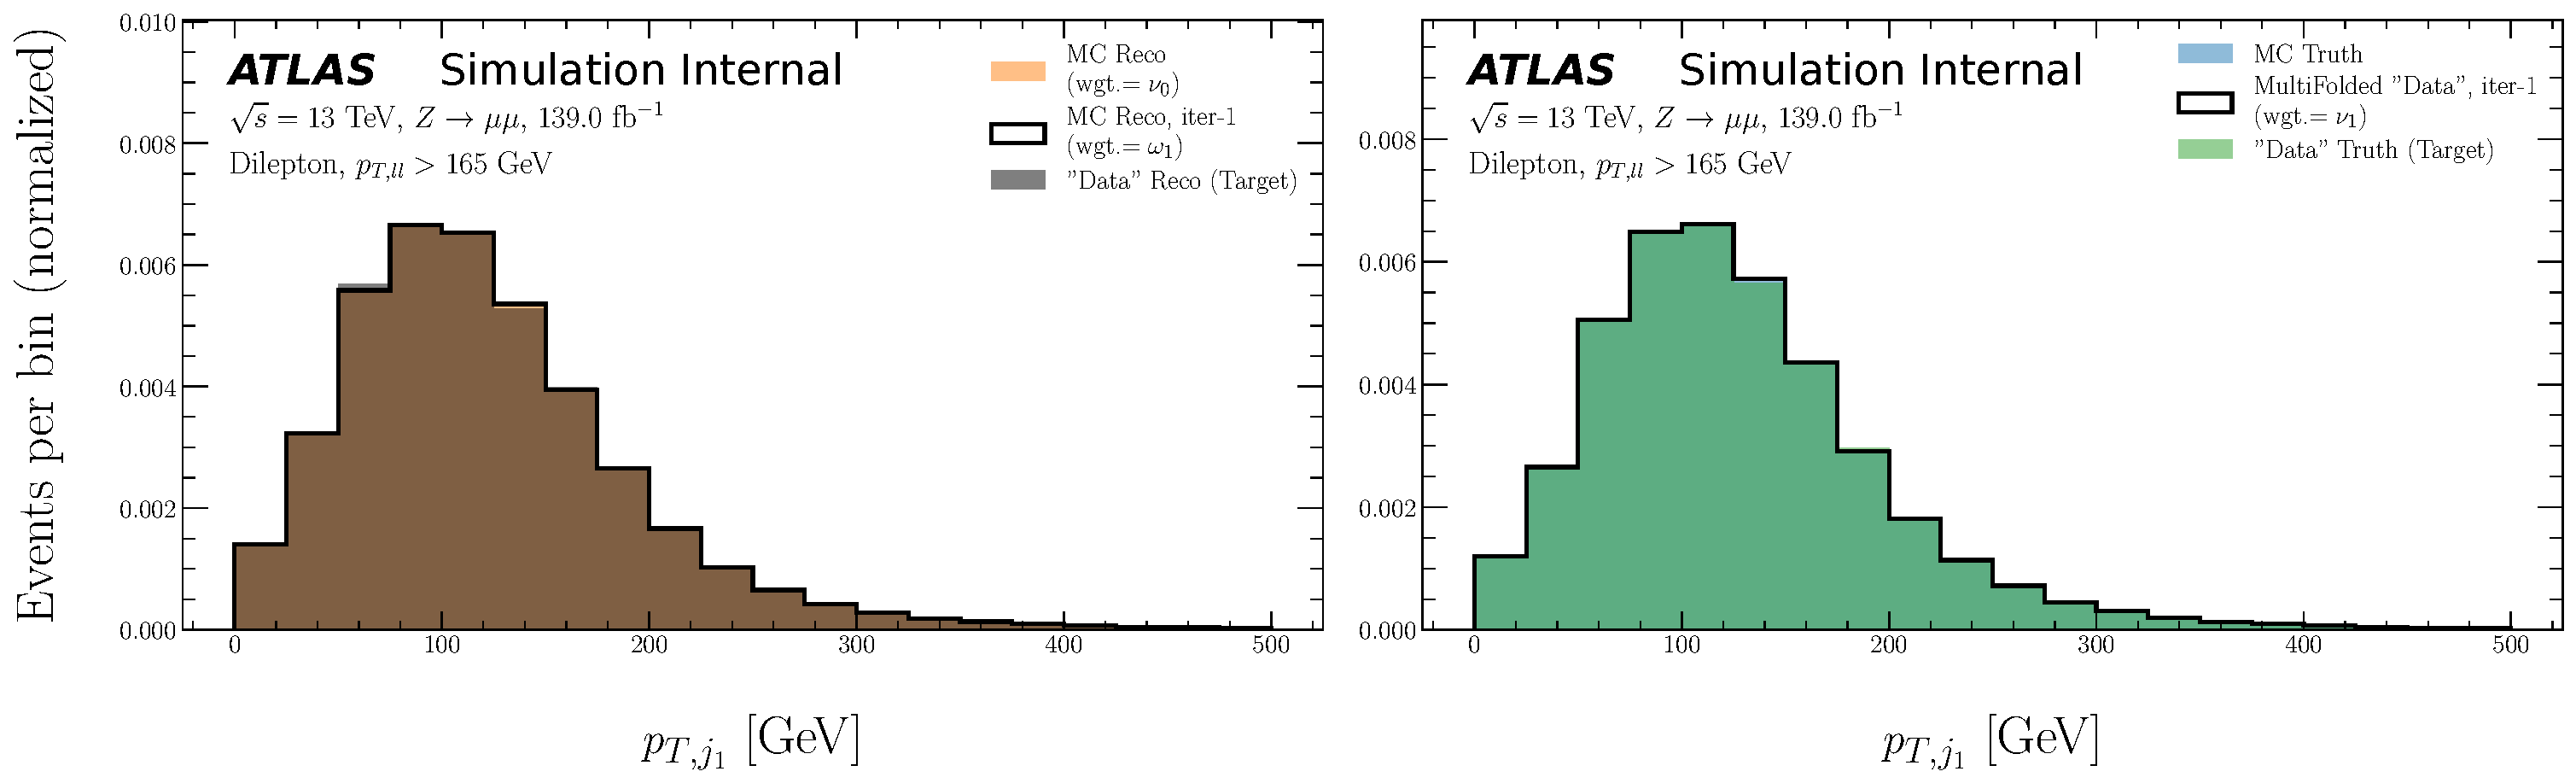
\includegraphics[width=0.95\textwidth]{figures/ATLASOmniFold-StressTest/ATLASOmniFold-TechnicalClosureTest/MultiFold/pT_trackj1/ATLASOmniFold-TechnicalClosureTest-MultiFold-pT_trackj1-Iteration01.pdf}}
\caption{A technical closure test for the $p_T$ of the leading track jet using MultiFold (16 observables are simultaneously unfolded).  The top plot show the input histograms and the bottom plots are the results after one iteration of OmniFold.  By construction the top left and top right histograms are statistically identical.}
\label{fig:technicalclosureMulti:pT_trackj1}
\end{figure}

\begin{figure}[h!]
\centering
\subfloat[Input histograms]{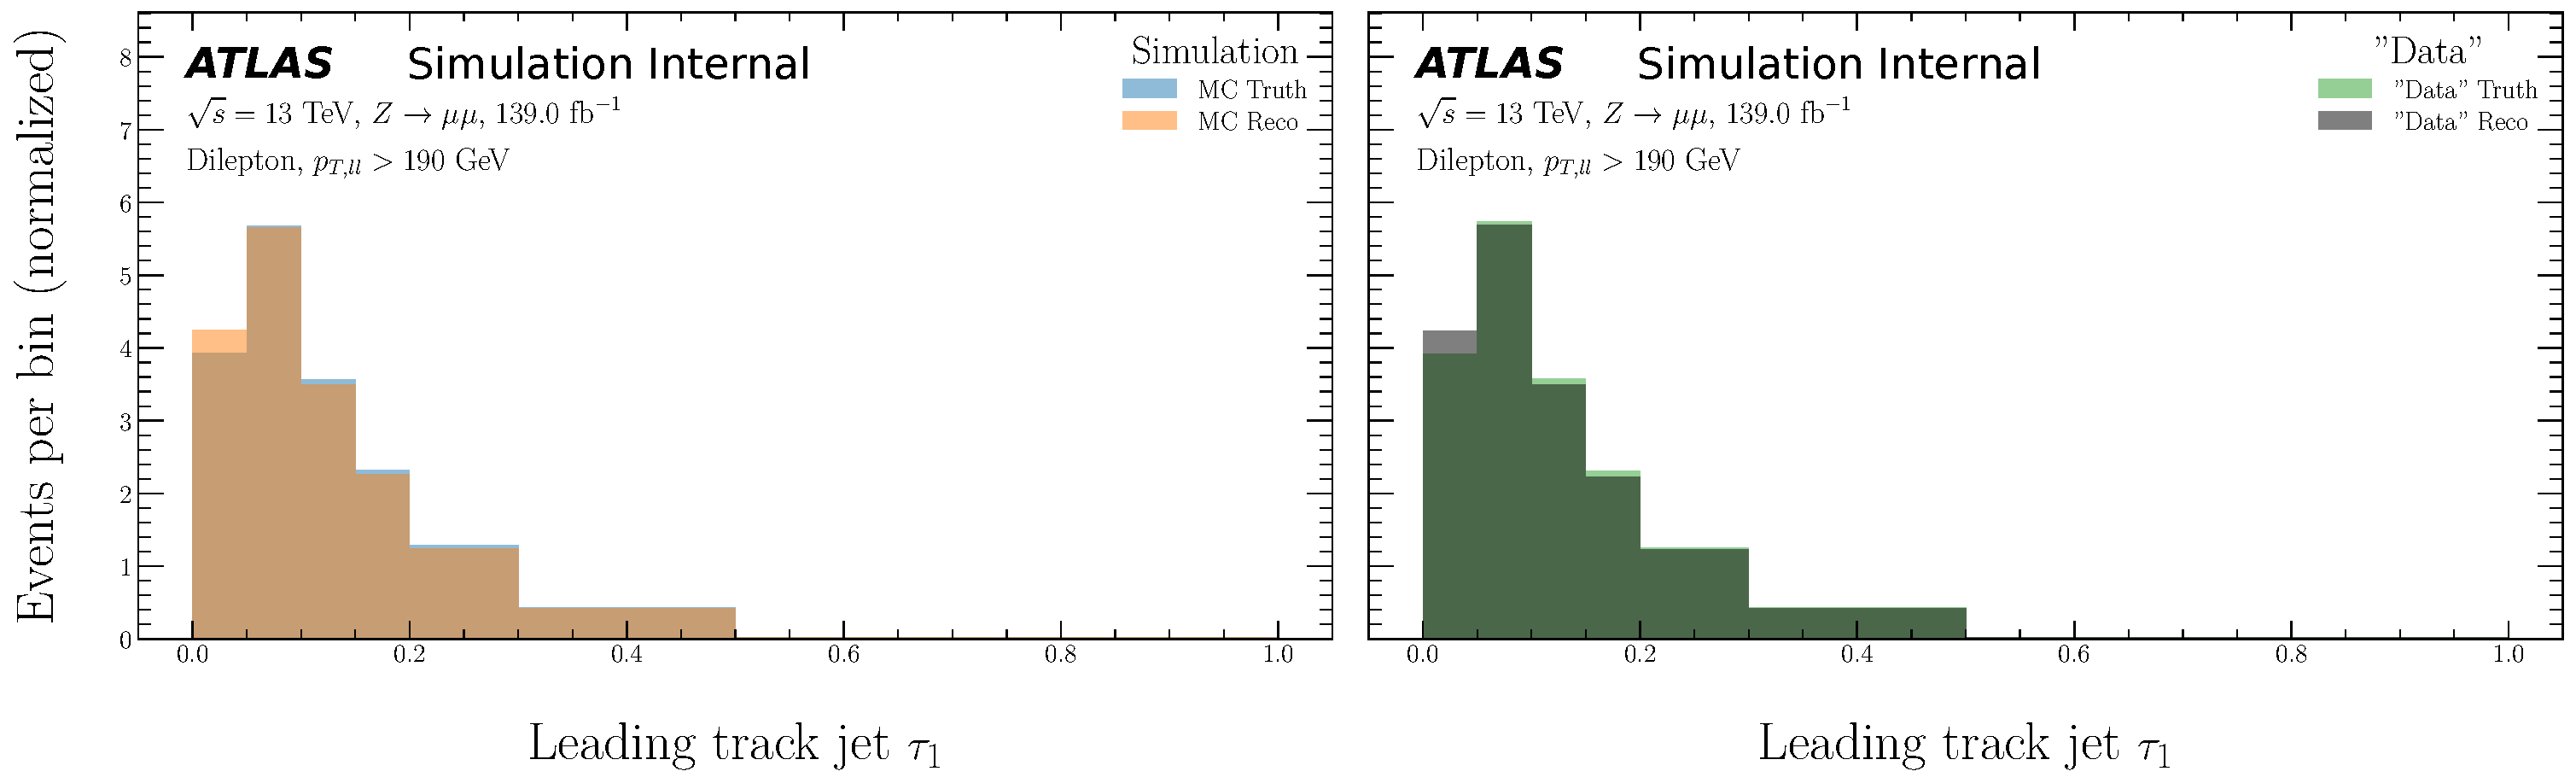
\includegraphics[width=0.89\textwidth]{figures/ATLASOmniFold-StressTest/ATLASOmniFold-TechnicalClosureTest/MultiFold/tau1_trackj1/ATLASOmniFold-TechnicalClosureTest-MultiFold-tau1_trackj1-Distributions.pdf}}\\
\subfloat[After 1 iteration]{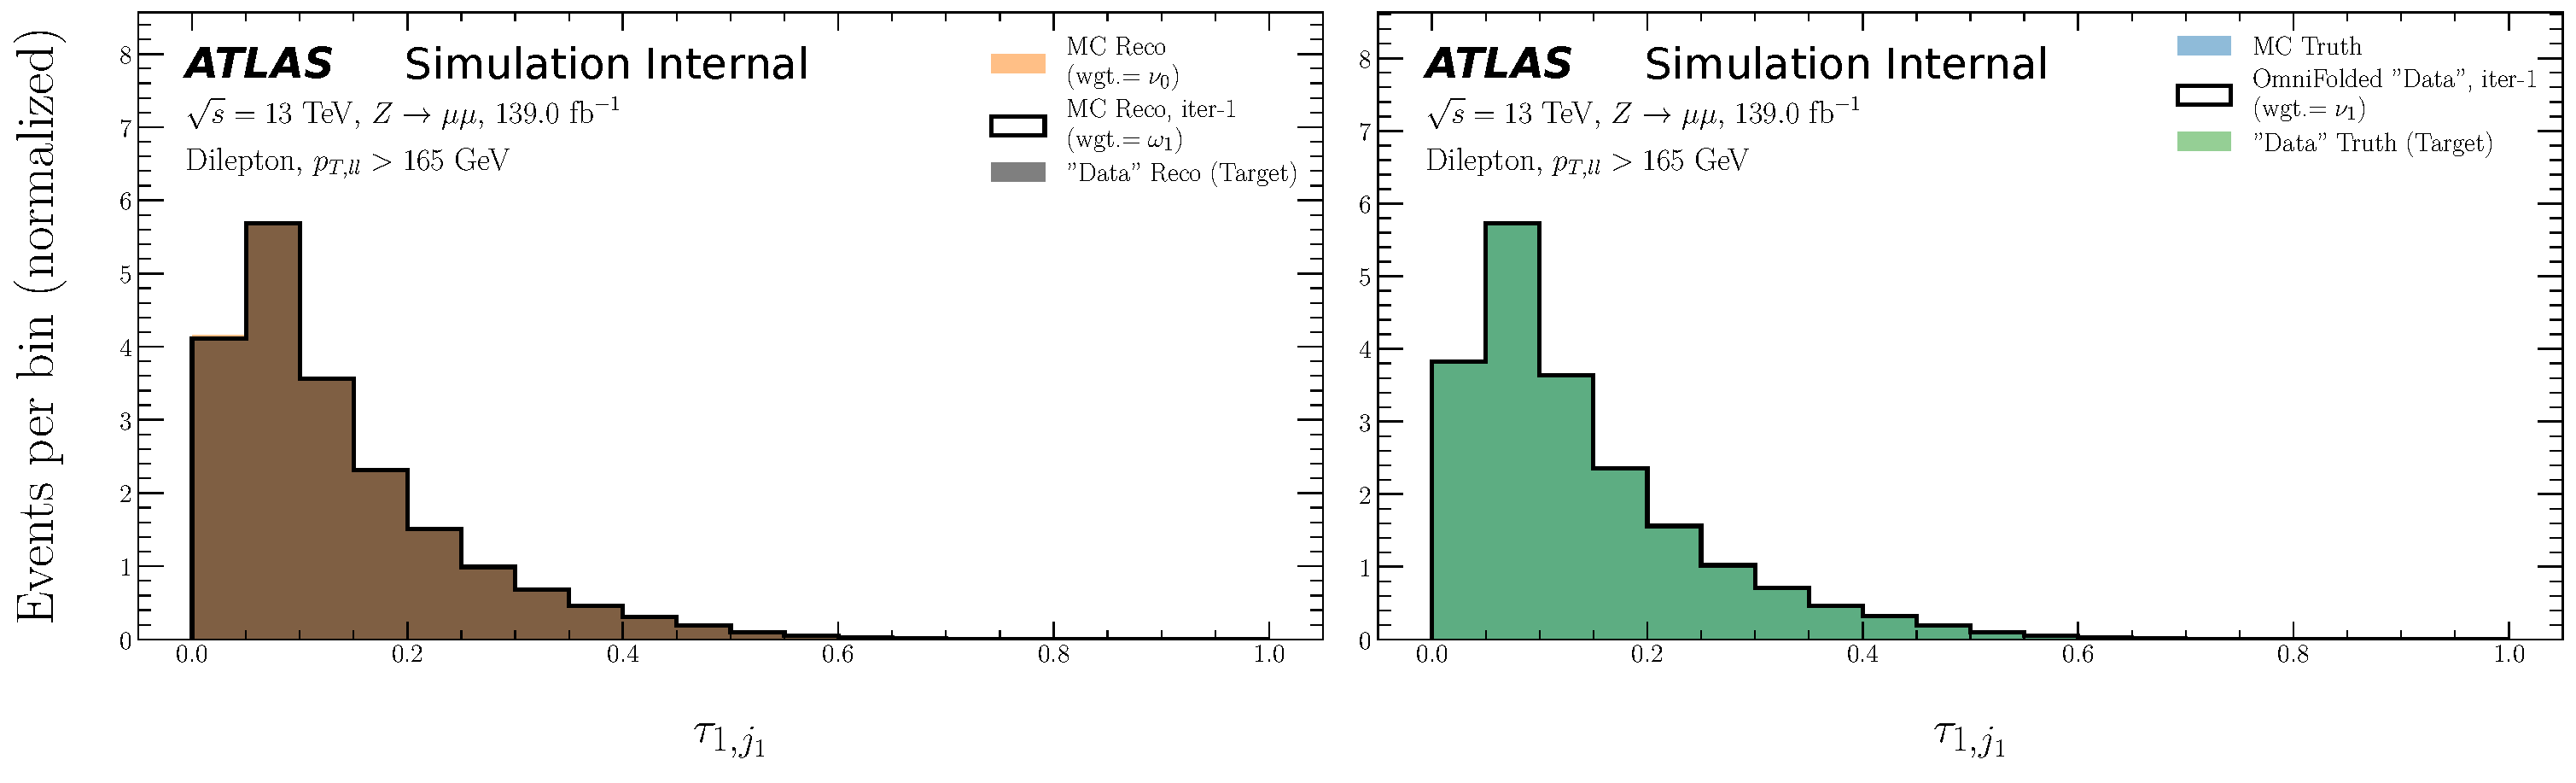
\includegraphics[width=0.95\textwidth]{figures/ATLASOmniFold-StressTest/ATLASOmniFold-TechnicalClosureTest/MultiFold/tau1_trackj1/ATLASOmniFold-TechnicalClosureTest-MultiFold-tau1_trackj1-Iteration01.pdf}}
\caption{A technical closure test for the $\tau_1$ of the leading track jet using MultiFold (16 observables are simultaneously unfolded).  The top plot show the input histograms and the bottom plots are the results after one iteration of OmniFold.  By construction the top left and top right histograms are statistically identical.}
\label{fig:technicalclosureMulti:tau1_trackj1}
\end{figure}

\begin{figure}[h!]
\centering
\subfloat[Input histograms]{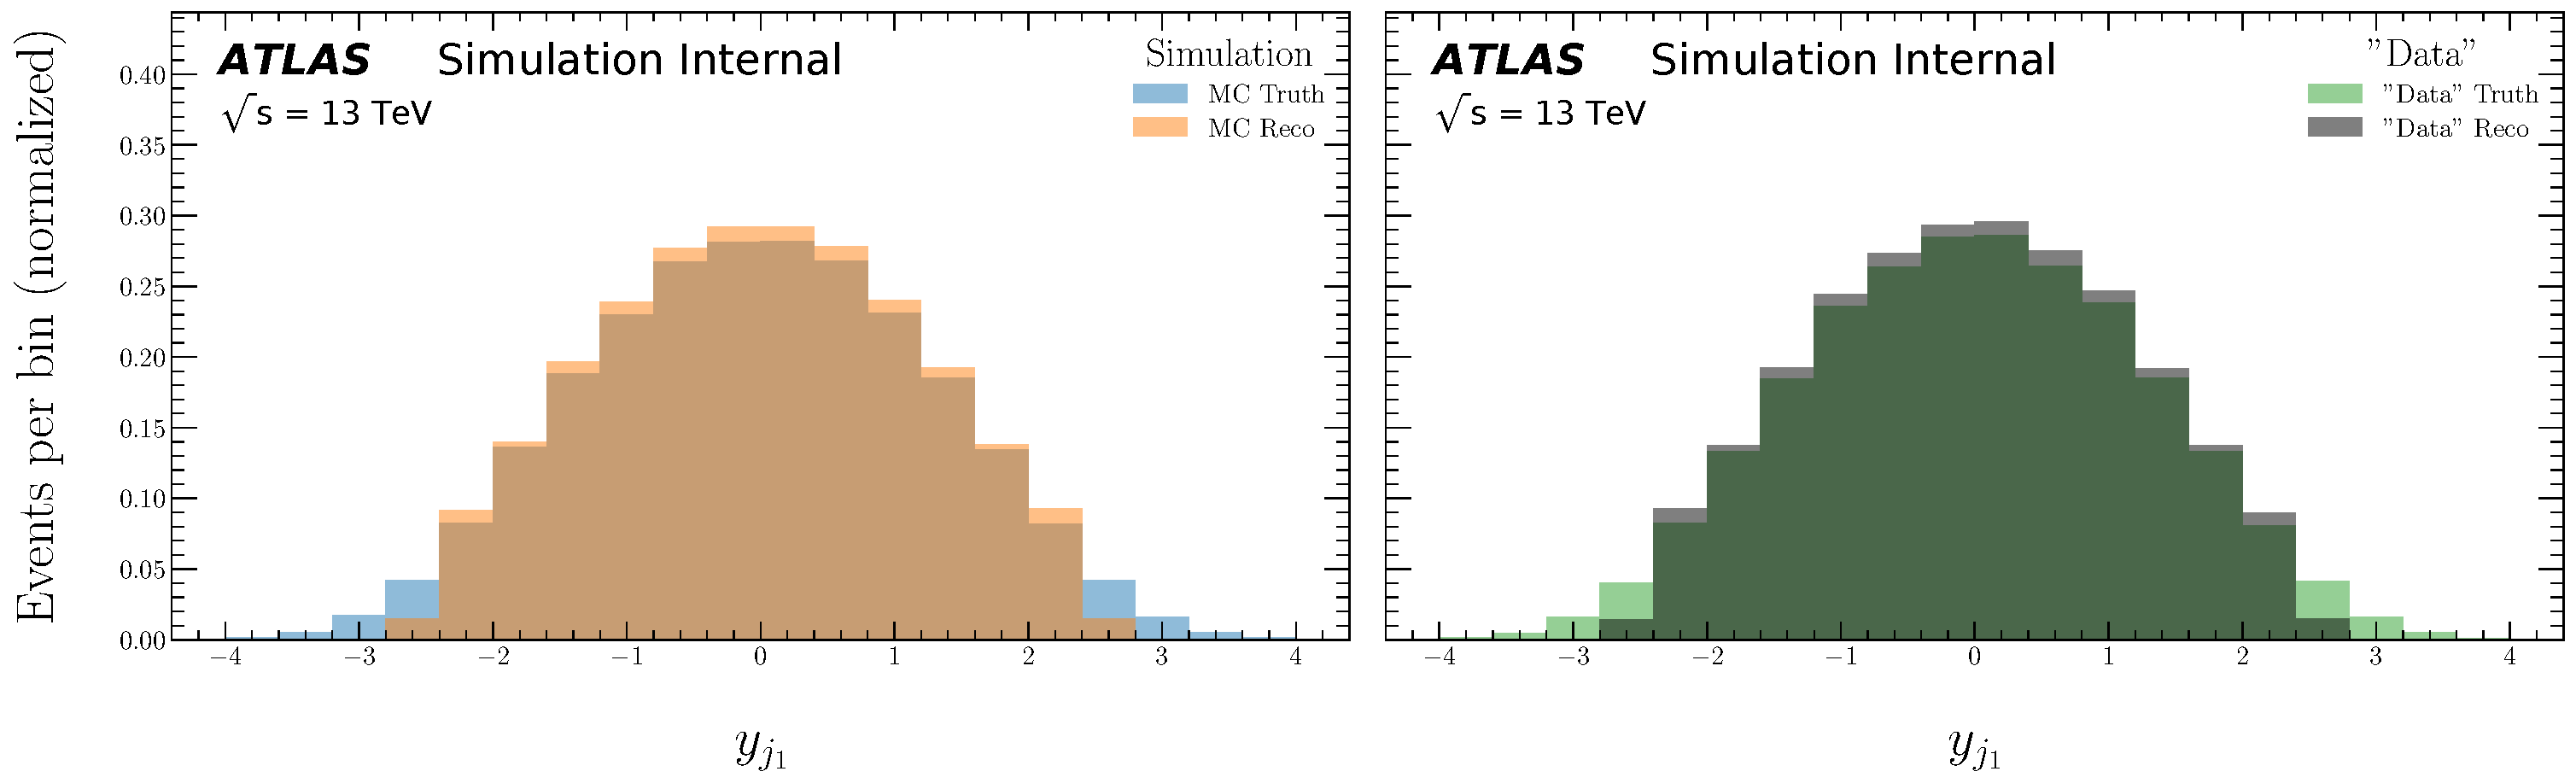
\includegraphics[width=0.95\textwidth]{figures/ATLASOmniFold-StressTest/ATLASOmniFold-TechnicalClosureTest/MultiFold/y_trackj1/ATLASOmniFold-TechnicalClosureTest-MultiFold-y_trackj1-Distributions.pdf}}\\
\subfloat[After 1 iteration]{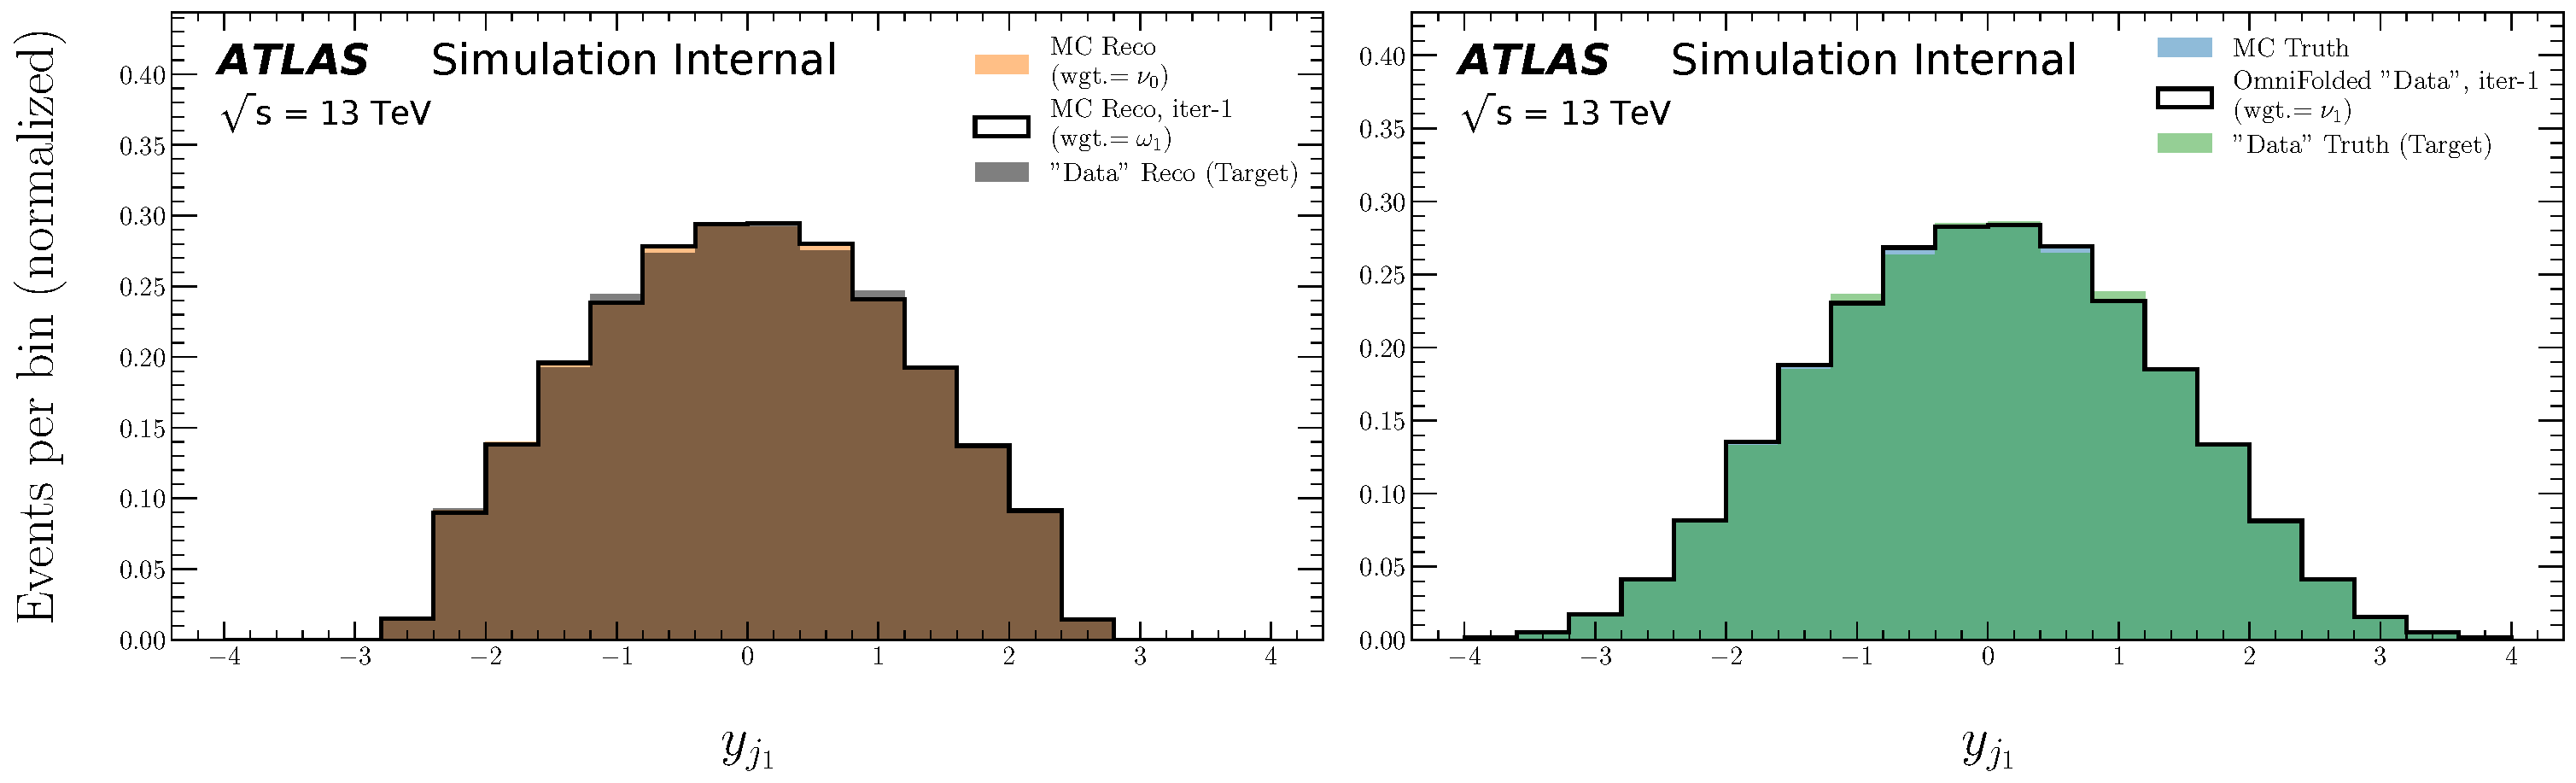
\includegraphics[width=0.95\textwidth]{figures/ATLASOmniFold-StressTest/ATLASOmniFold-TechnicalClosureTest/MultiFold/y_trackj1/ATLASOmniFold-TechnicalClosureTest-MultiFold-y_trackj1-Iteration01.pdf}}
\caption{A technical closure test for the rapidity of the leading track jet using MultiFold (16 observables are simultaneously unfolded).  The top plot show the input histograms and the bottom plots are the results after one iteration of OmniFold.  By construction the top left and top right histograms are statistically identical.}
\label{fig:technicalclosureMulti:y_trackj1}
\end{figure}

\subsection{Artificial Stress Tests}
\label{sec:technicalclosure2}

In this section, we apply artificial weights to the events in order to shift the various distributions and we show that we can recover the unshifted distributions.  In particular, we divide the Pythia sample in half again and apply stress weights to the half labeled `simulation'.  In one case (Sec.~\ref{sec:stress:deterministic}), these weights are a deterministic function of the input features.  In a second case (Sec.~\ref{sec:stress:stochastic}), the weights are stochastic function of the inputs.

\clearpage

\subsubsection{Deterministic Weights}
\label{sec:stress:deterministic}

For a given event $x$ in sample $X$, the stress weights are given by 

\begin{align}
\label{eq:stressweights}
w = w_{MC}\,(-\min_{x'\in X}\mathcal{Z}(x')+\mathcal{Z}(x))^n\,,
\end{align}
%
where $w_{MC}$ is the Monte Carlo event weight and $\mathcal{Z}$ gives the Z-score of $x\in X$. We do a basic weight standardization given all stress weights $W$ by doing $w\mapsto\frac{w}{\langle W\rangle}$. These stress weights are constructed to induce a right shift in the given distribution. Note that a larger value of $n$ induces a more intense right-shift in the stressed distributions.  For the UniFold distributions, a value of $n=2$ is used; for the MultiFold distributions, we use $n=3$.

\paragraph{UniFold}

Figures~\ref{fig:stressa_mass} and~\ref{fig:stressa_Ntracks_trackj1} are examples for the leading track jet mass and the number of tracks inside jets.  Additional examples can be found in App~\ref{sec:stressunifolddet}.

\begin{figure}[h!]
\centering
\subfloat[Weights]{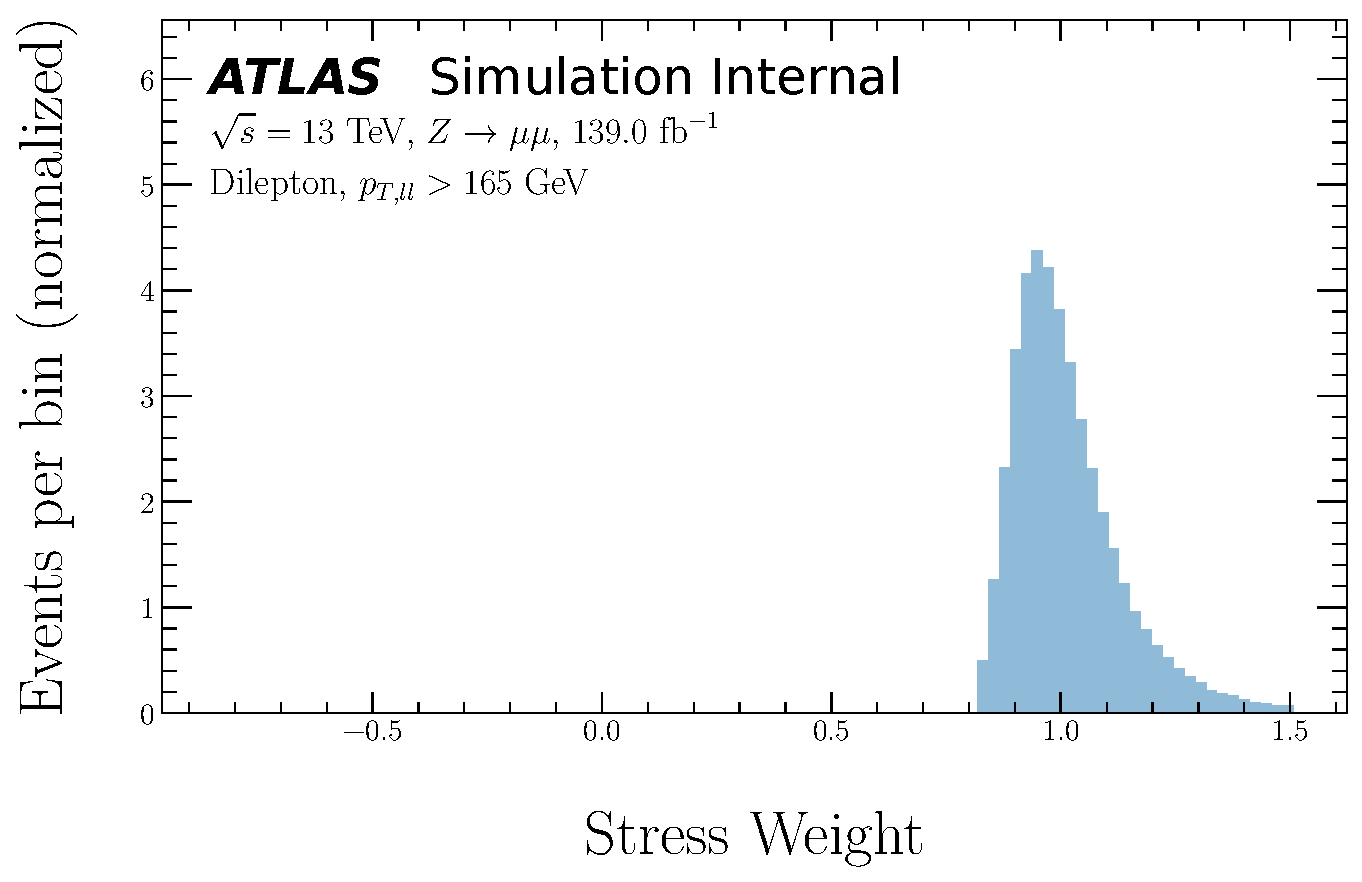
\includegraphics[width=0.45\textwidth]{figures/ATLASOmniFold-StressTest/ATLASOmniFold-StressTestA/UniFold/m_trackj1/ATLASOmniFold-StressTestA-UniFold-m_trackj1-StressWeightsHist.pdf}}\\
\subfloat[Input histograms]{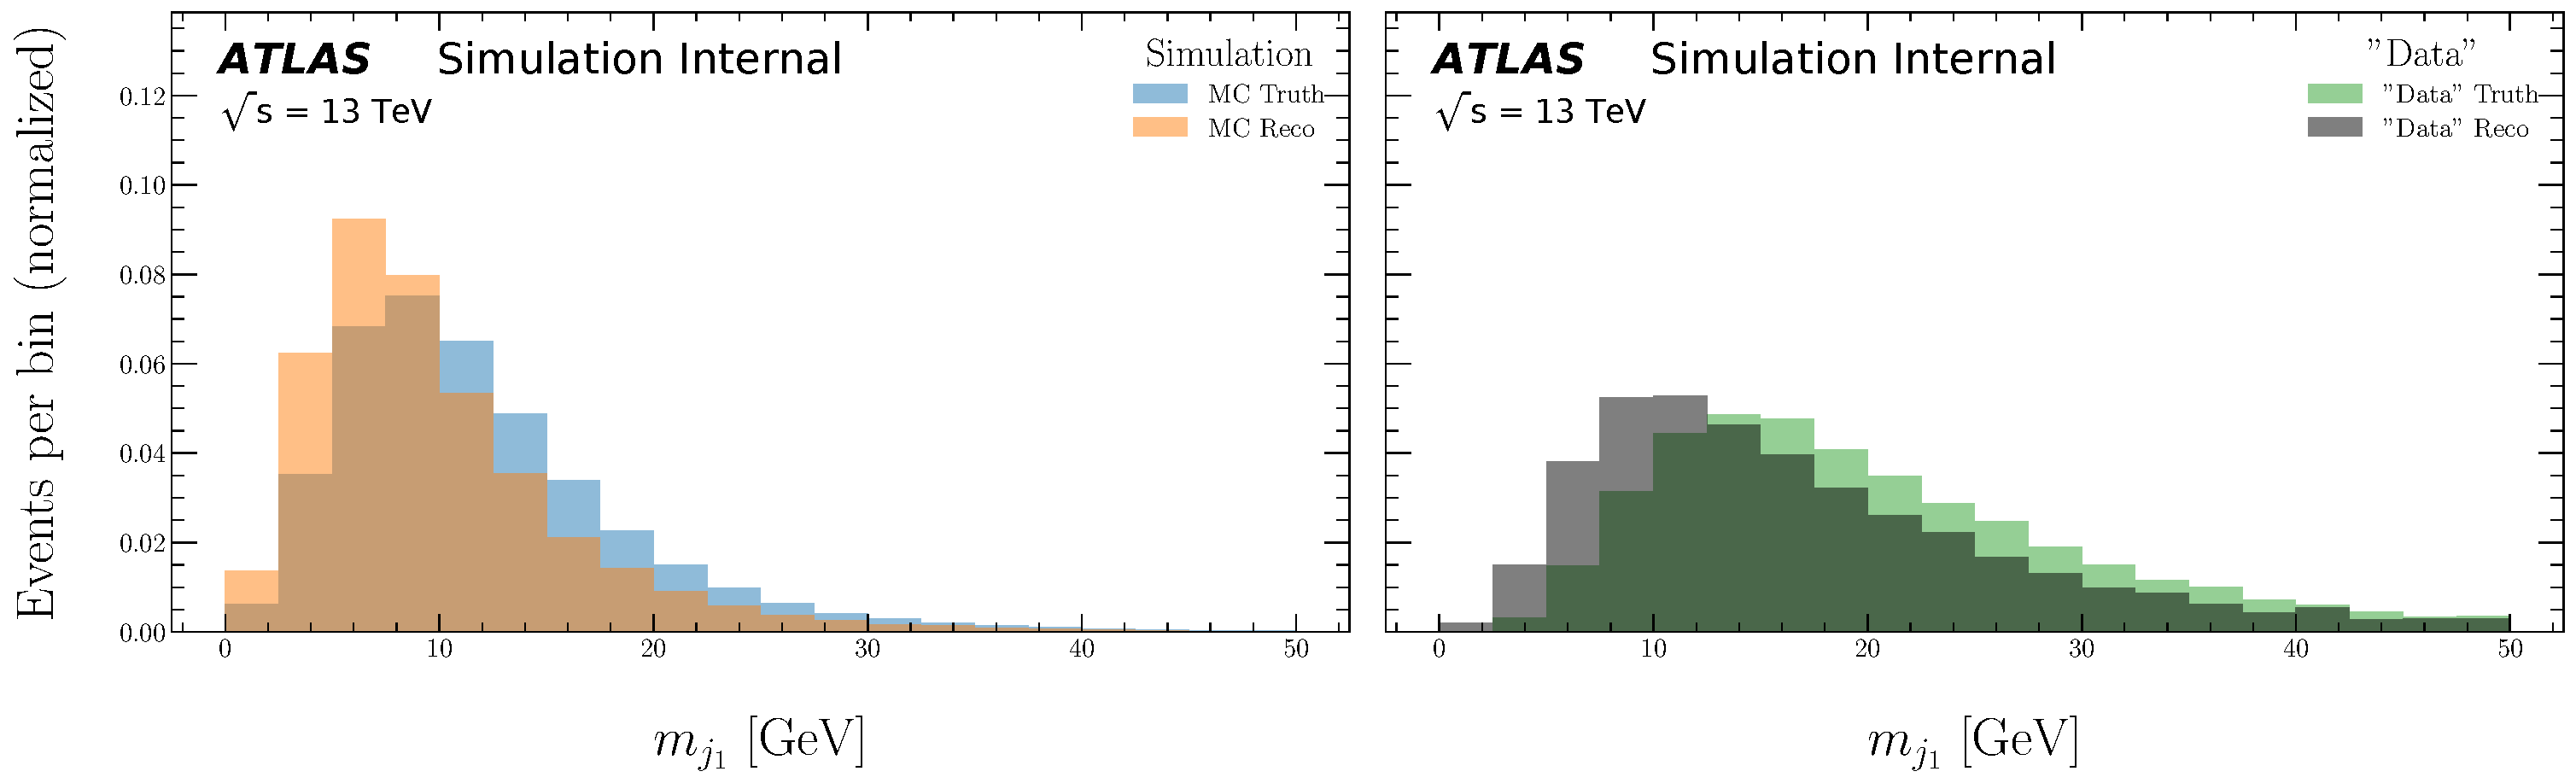
\includegraphics[width=0.85\textwidth]{figures/ATLASOmniFold-StressTest/ATLASOmniFold-StressTestA/UniFold/m_trackj1/ATLASOmniFold-StressTestA-UniFold-m_trackj1-Distributions}}\\
\subfloat[After 1 iteration]{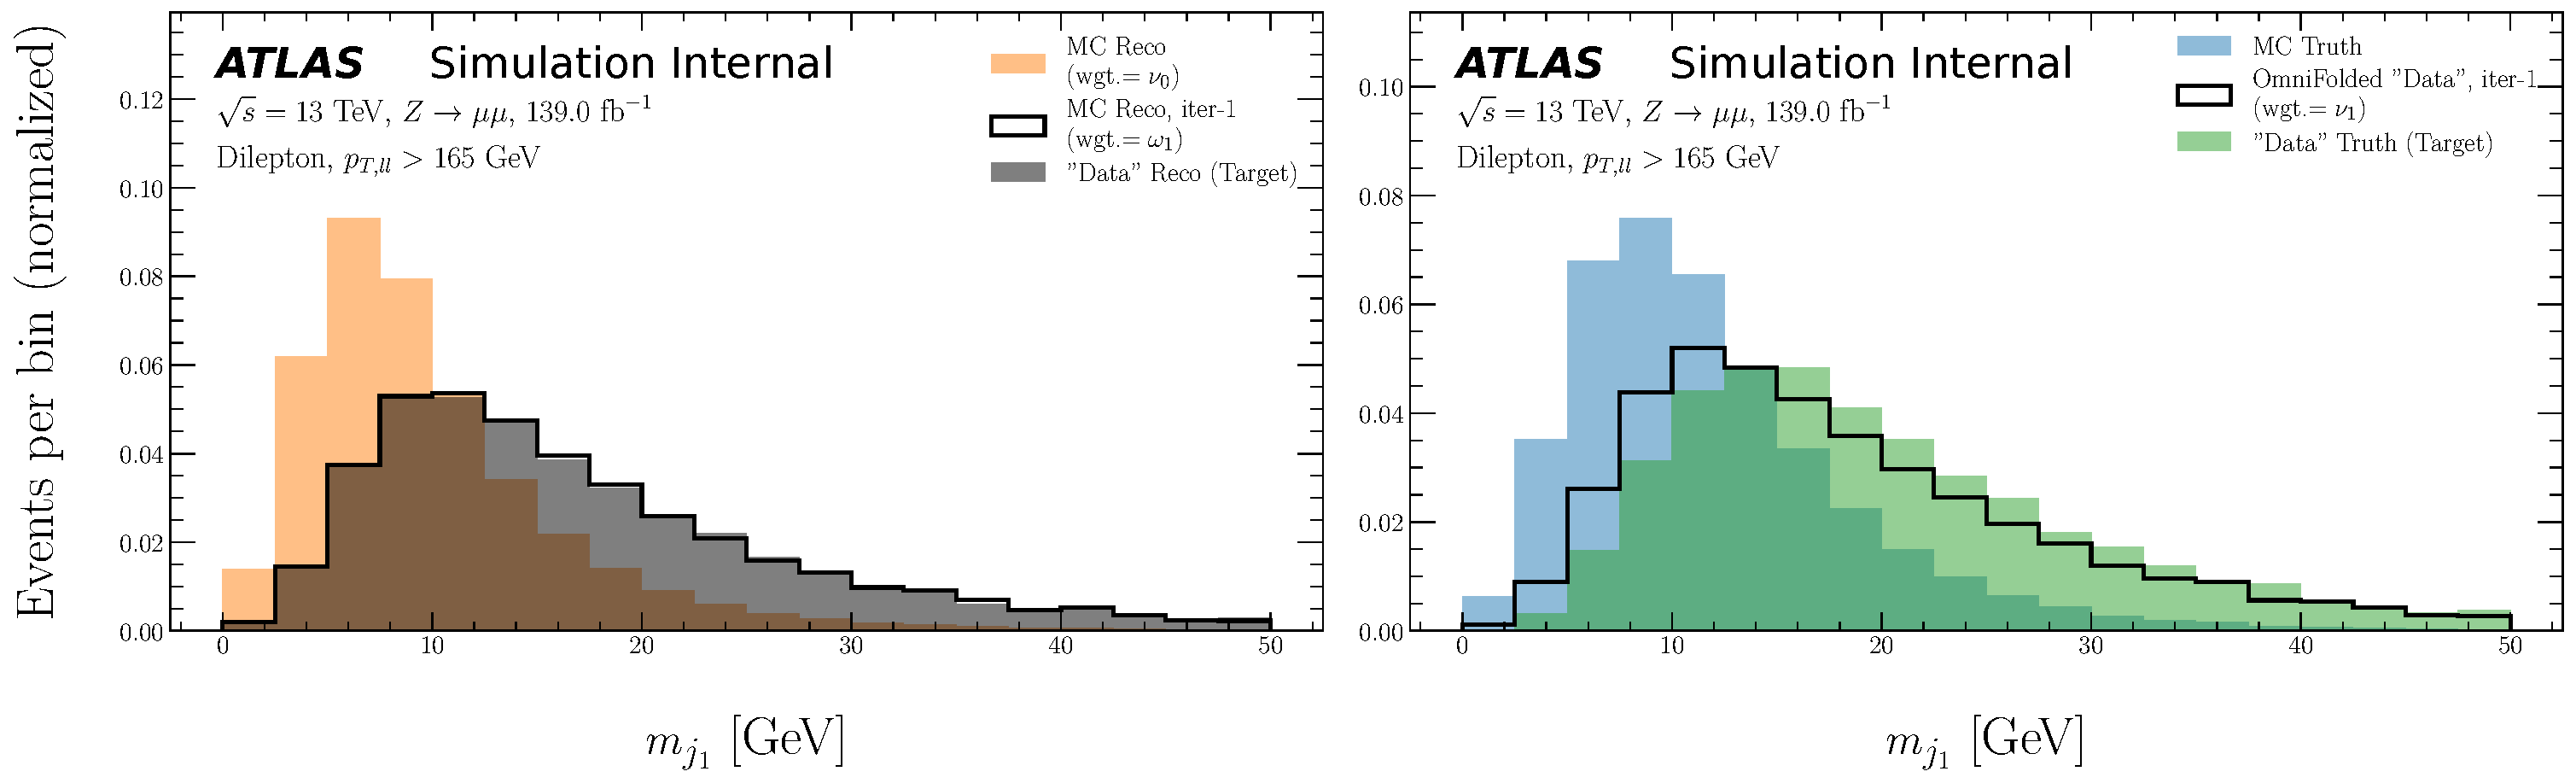
\includegraphics[width=0.85\textwidth]{figures/ATLASOmniFold-StressTest/ATLASOmniFold-StressTestA/UniFold/m_trackj1/ATLASOmniFold-StressTestA-UniFold-m_trackj1-Iteration01}}\\
\subfloat[After 2 iterations]{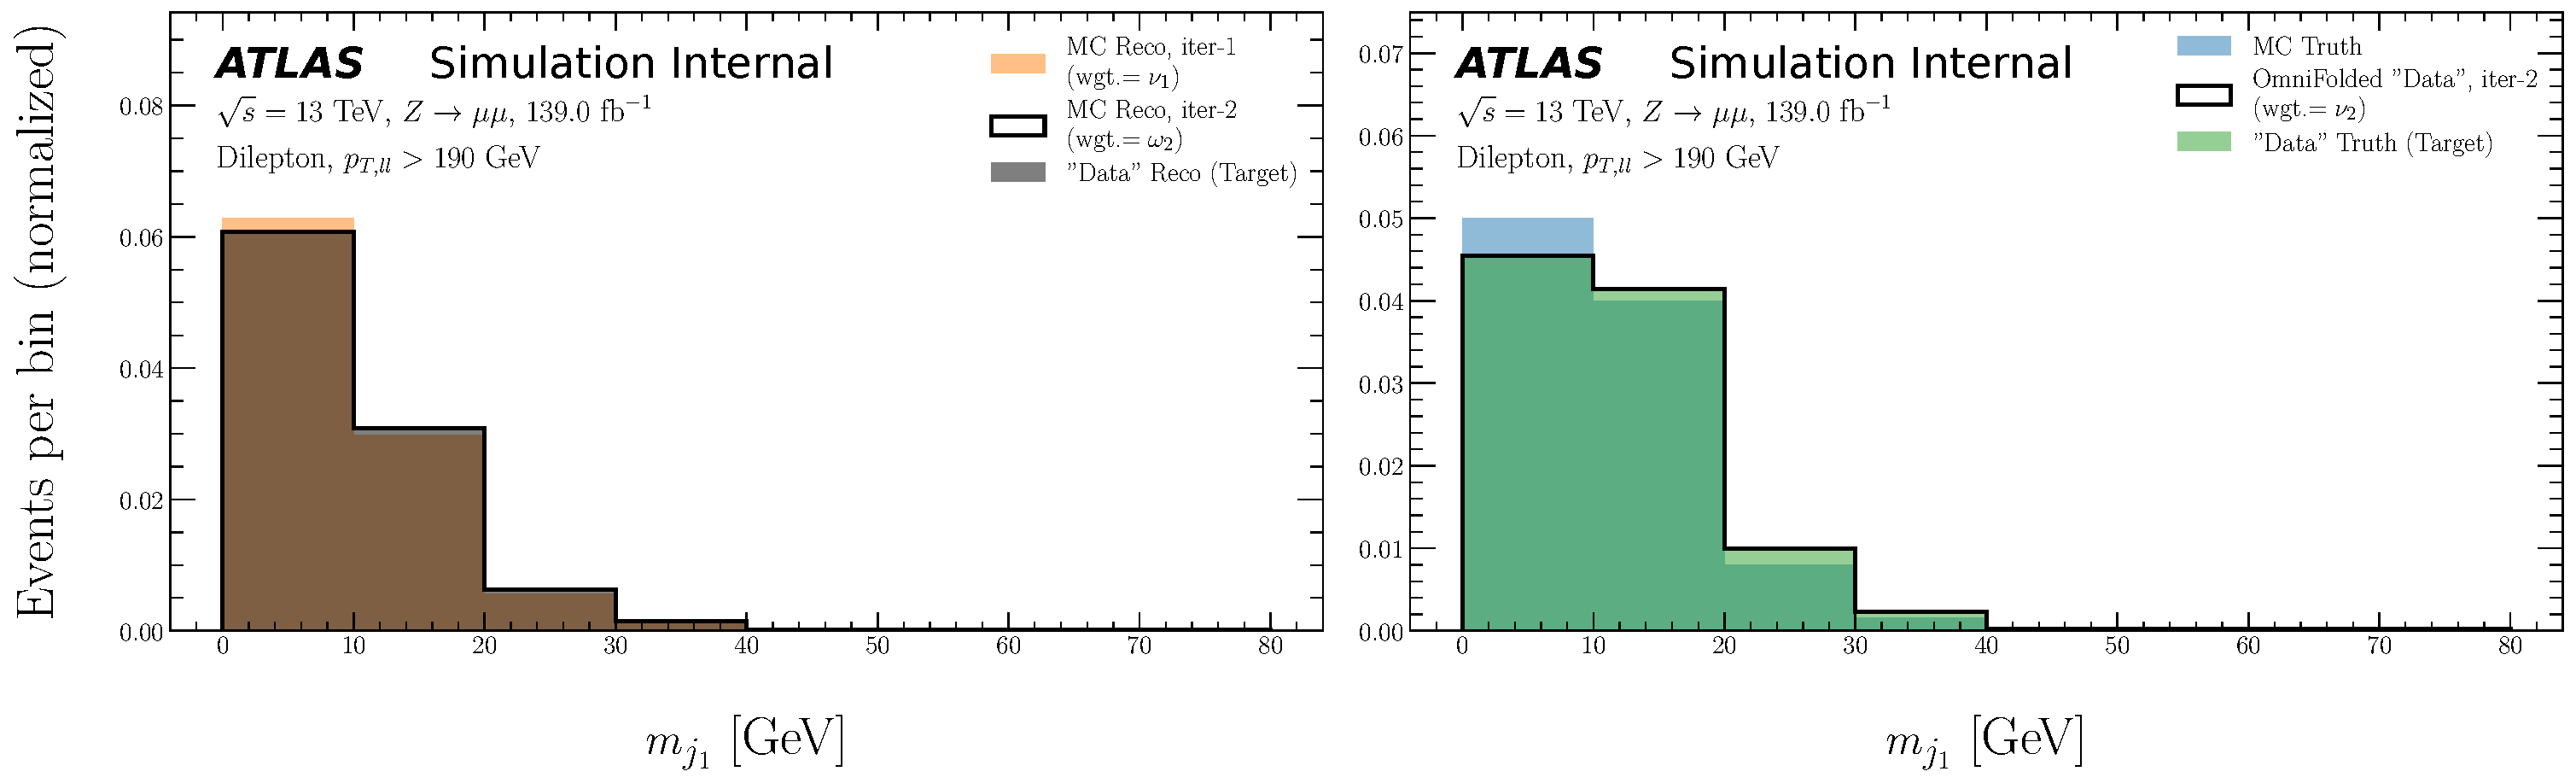
\includegraphics[width=0.85\textwidth]{figures/ATLASOmniFold-StressTest/ATLASOmniFold-StressTestA/UniFold/m_trackj1/ATLASOmniFold-StressTestA-UniFold-m_trackj1-Iteration02}}
\phantomcaption 
\end{figure}

\begin{figure}[h!]
\centering
\ContinuedFloat
\subfloat[After 3 iterations]{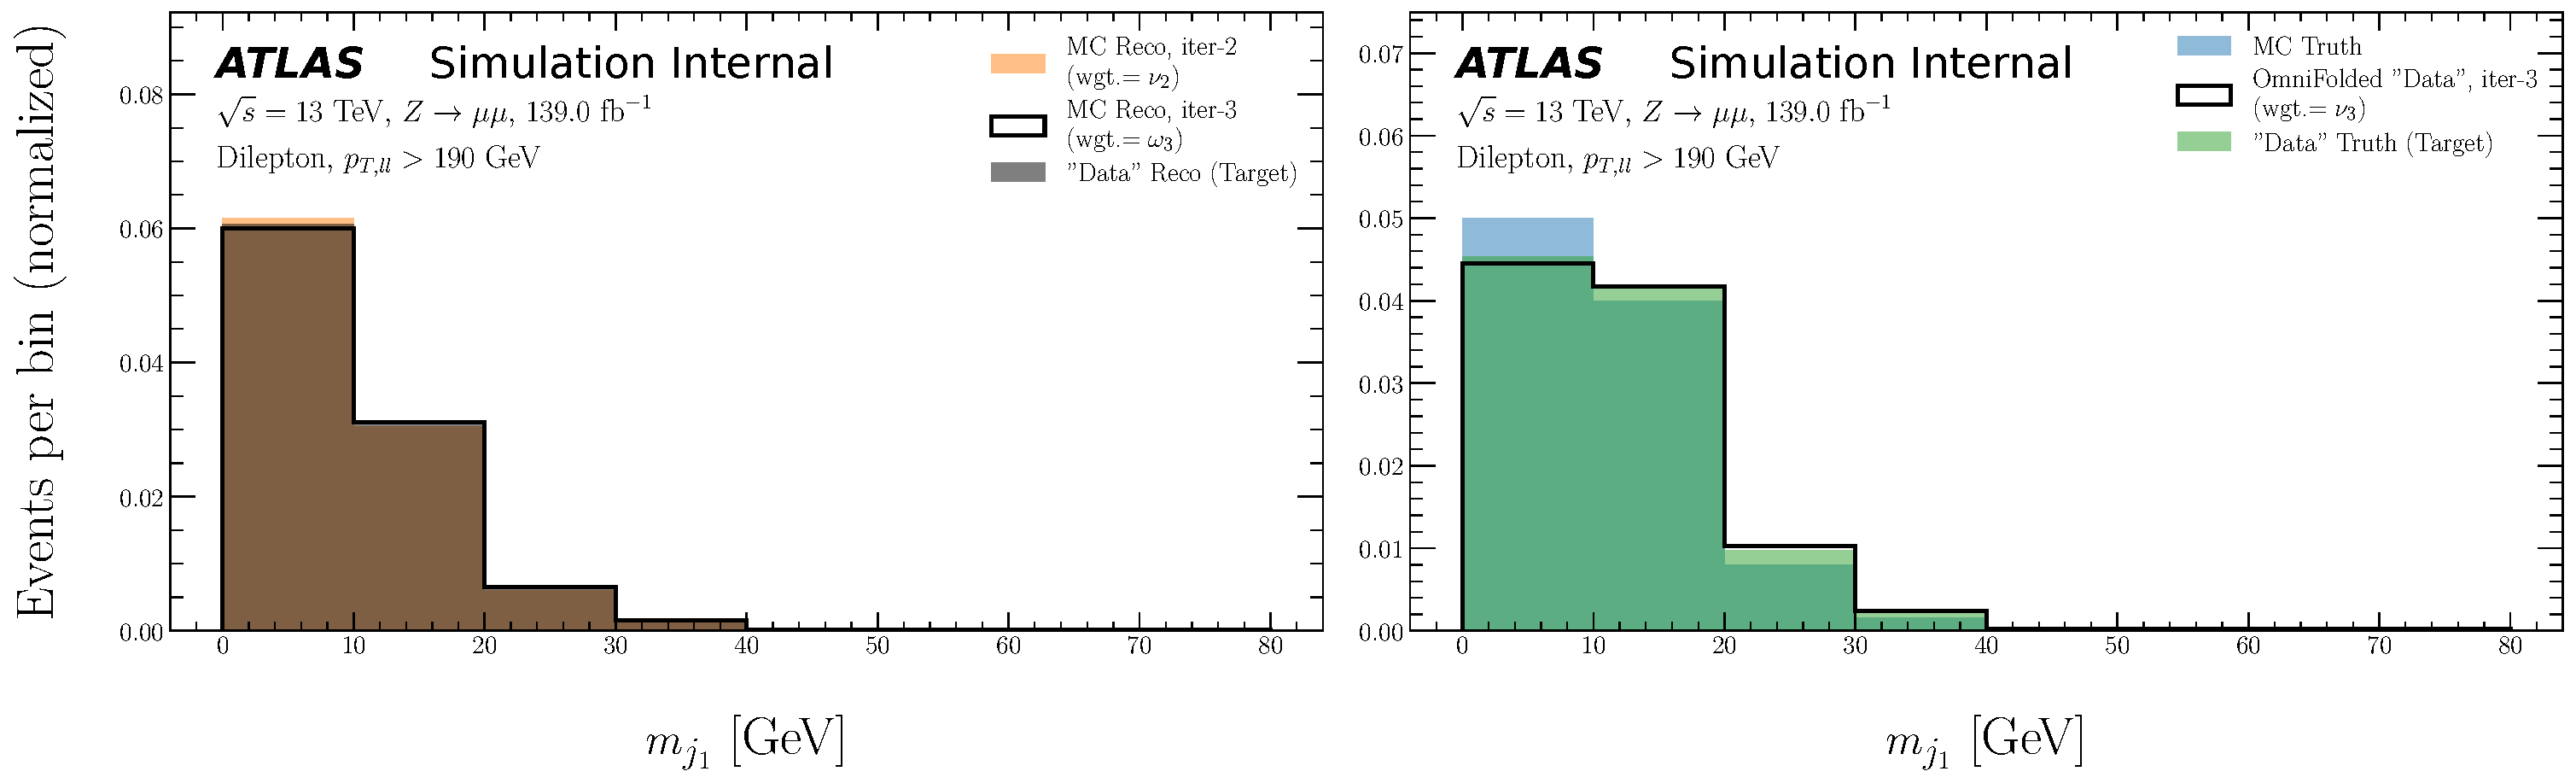
\includegraphics[width=0.85\textwidth]{figures/ATLASOmniFold-StressTest/ATLASOmniFold-StressTestA/UniFold/m_trackj1/ATLASOmniFold-StressTestA-UniFold-m_trackj1-Iteration03}}\\
\subfloat[After 4 iterations]{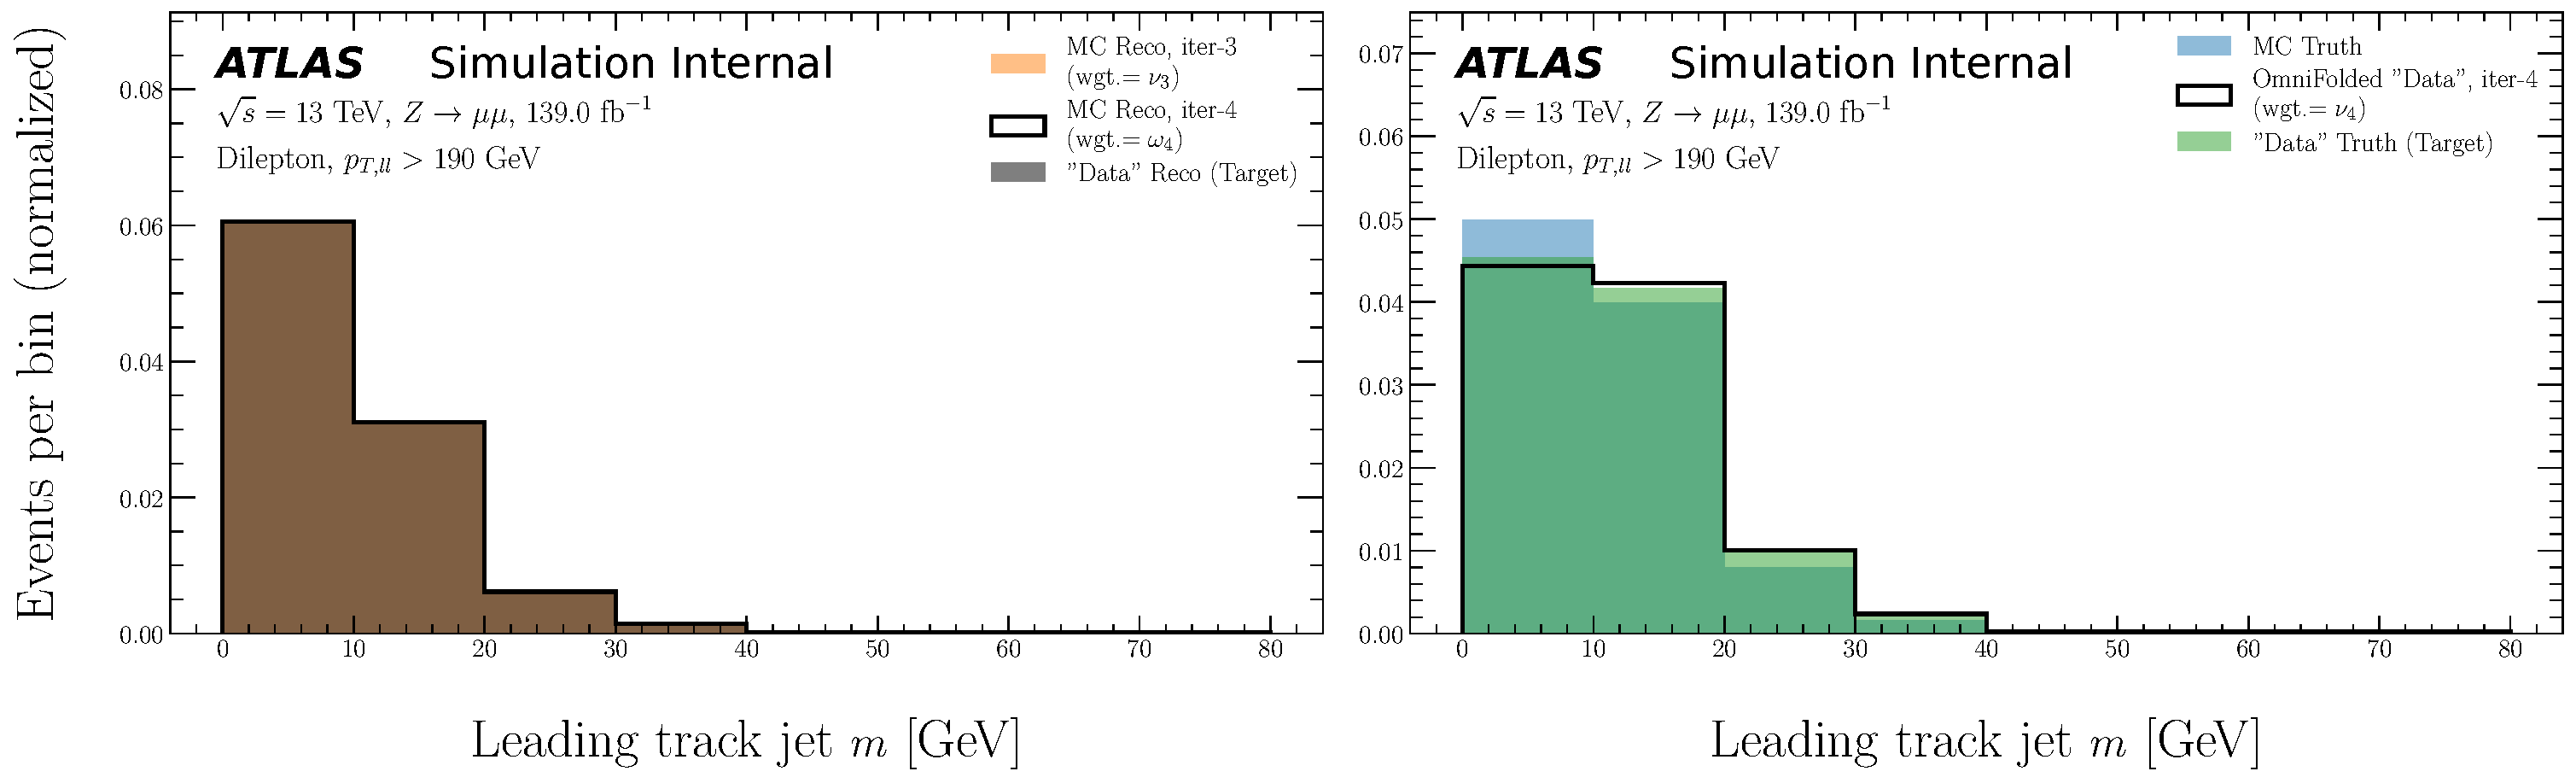
\includegraphics[width=0.85\textwidth]{figures/ATLASOmniFold-StressTest/ATLASOmniFold-StressTestA/UniFold/m_trackj1/ATLASOmniFold-StressTestA-UniFold-m_trackj1-Iteration04}}\\
\subfloat[After 5 iterations]{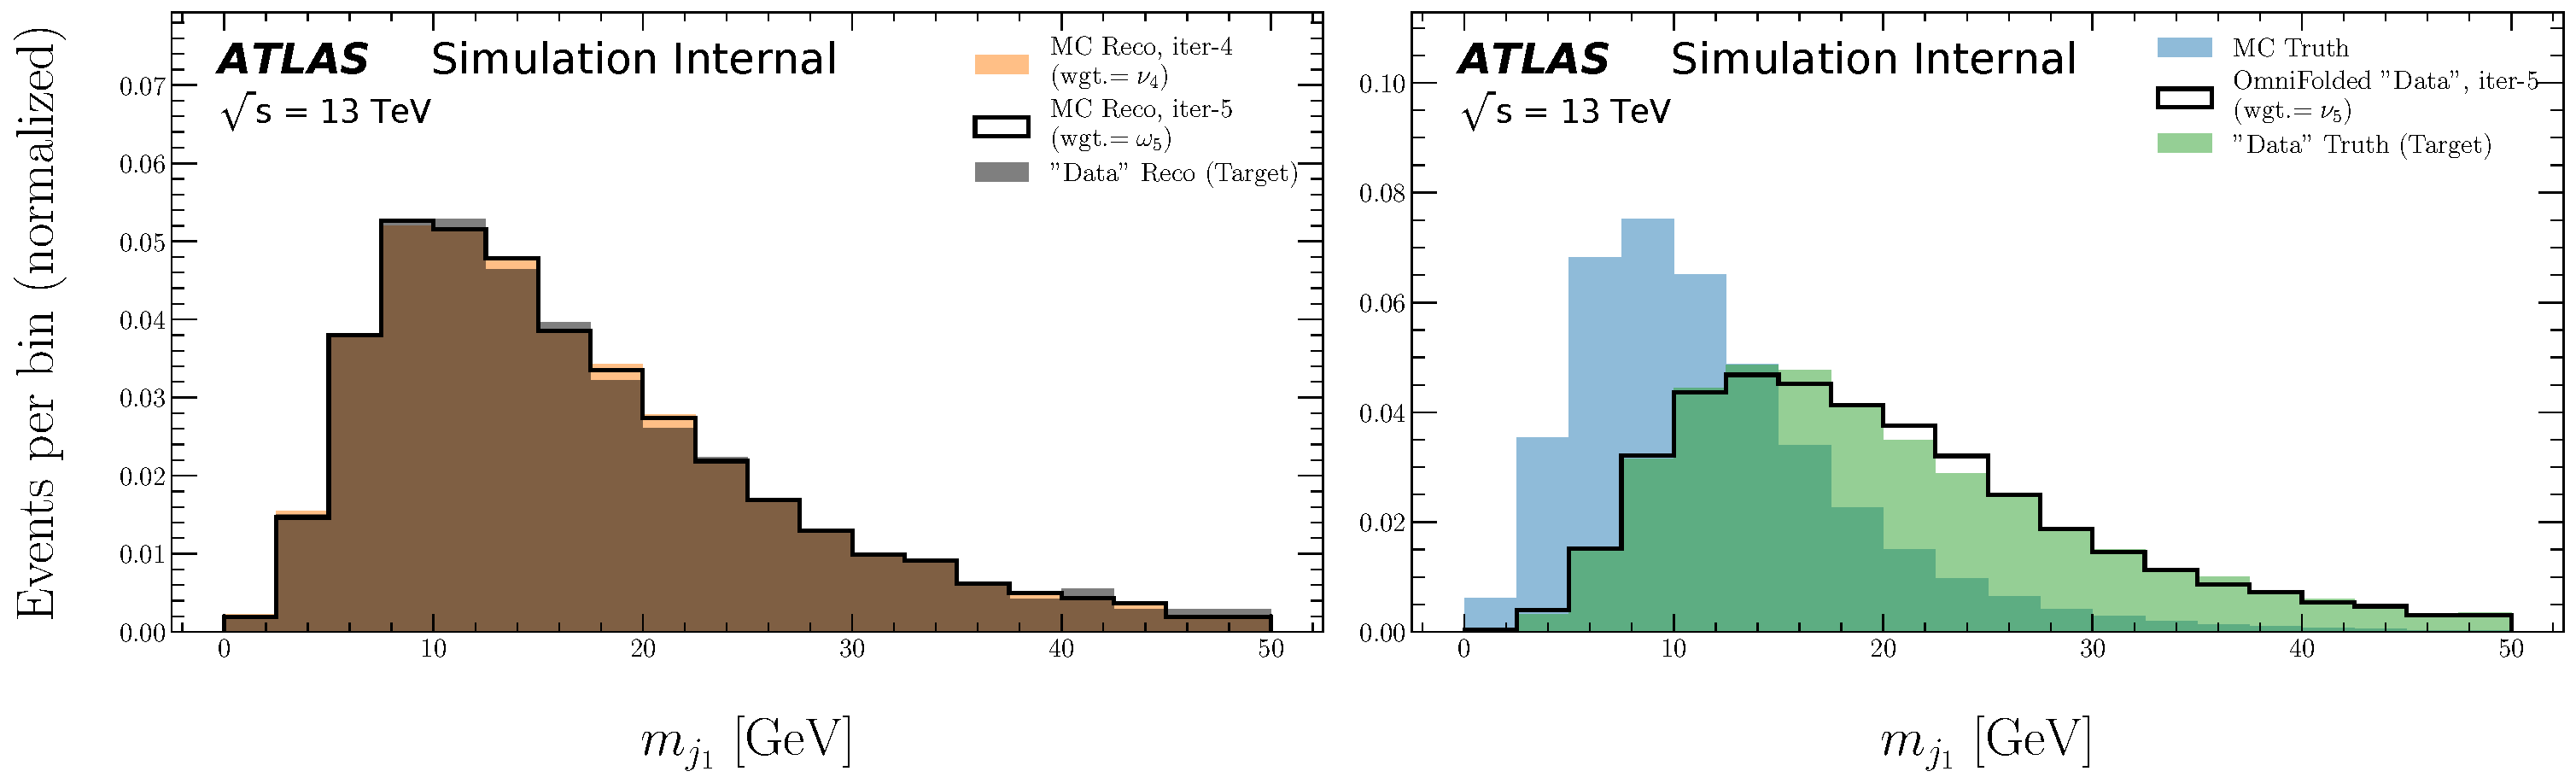
\includegraphics[width=0.85\textwidth]{figures/ATLASOmniFold-StressTest/ATLASOmniFold-StressTestA/UniFold/m_trackj1/ATLASOmniFold-StressTestA-UniFold-m_trackj1-Iteration05}}\\
\subfloat[After 6 iterations]{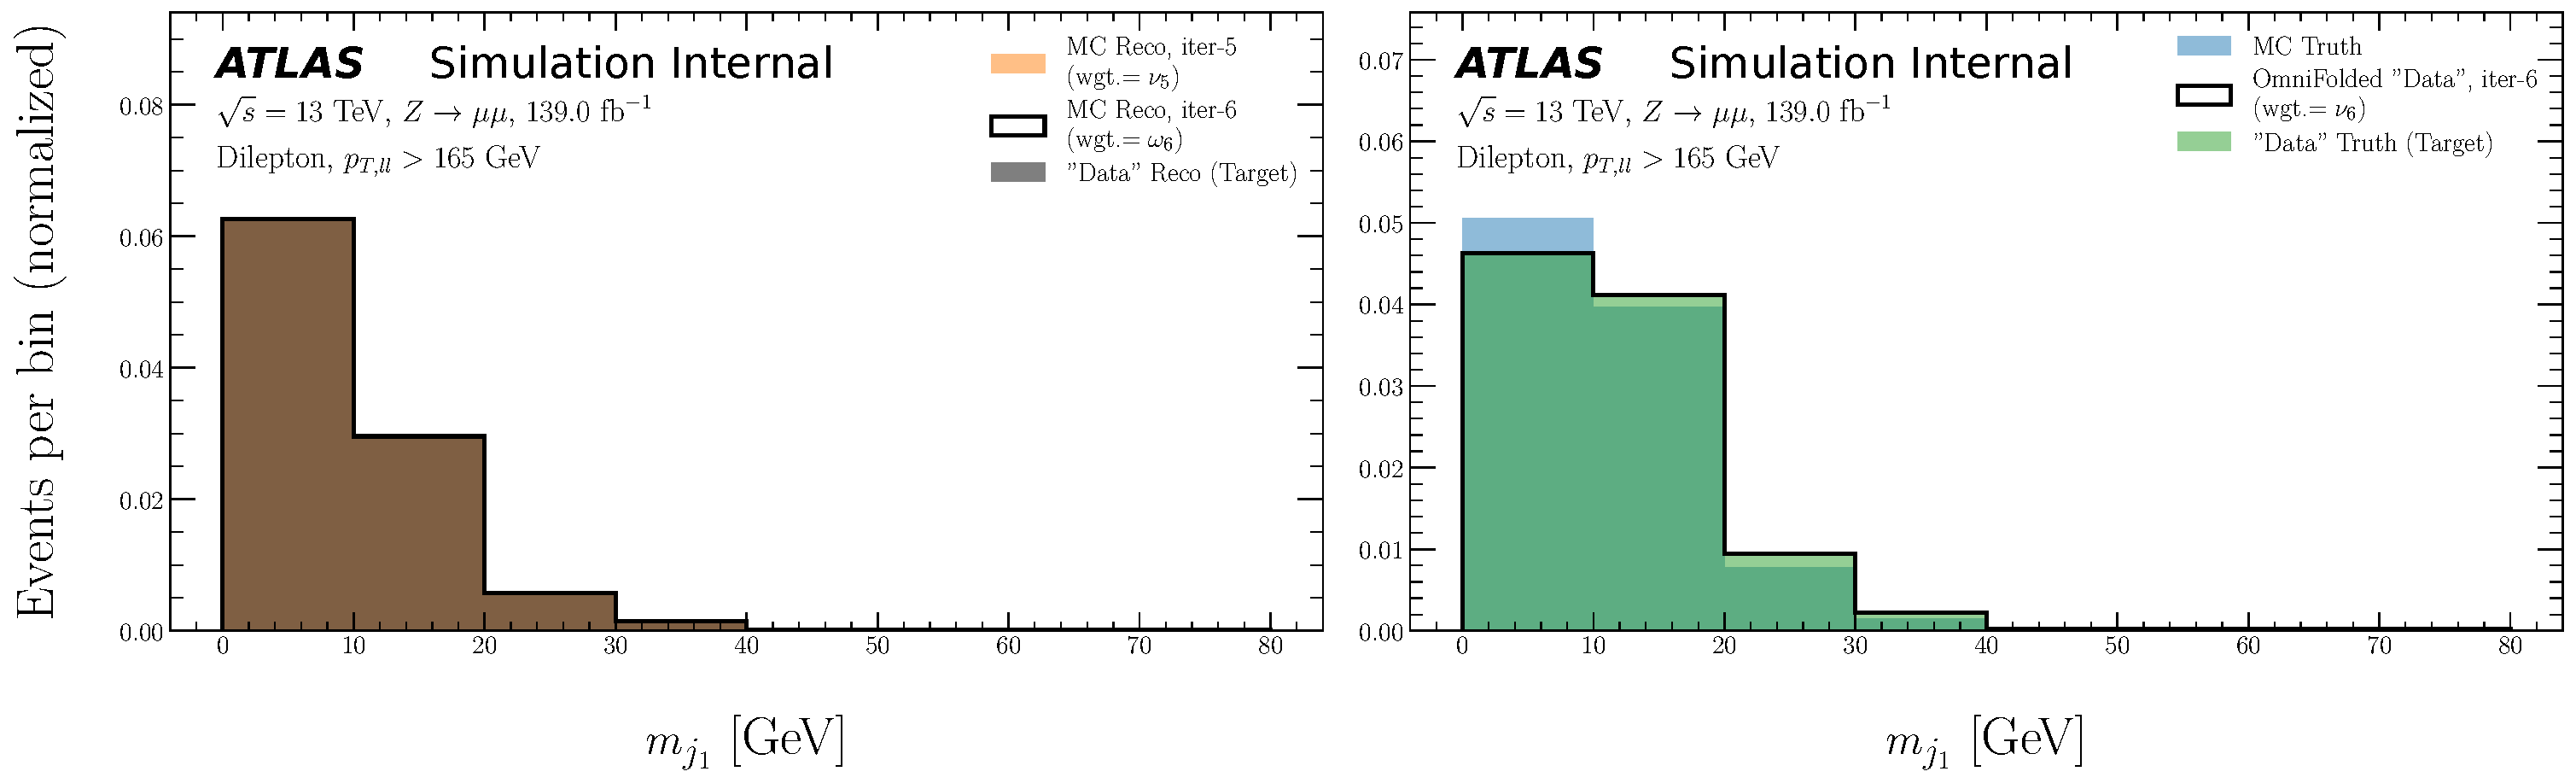
\includegraphics[width=0.85\textwidth]{figures/ATLASOmniFold-StressTest/ATLASOmniFold-StressTestA/UniFold/m_trackj1/ATLASOmniFold-StressTestA-UniFold-m_trackj1-Iteration06}}
\caption{A stress test for UniFold applied to the leading track jet mass.}
\label{fig:stressa_mass}
\end{figure}

\begin{figure}[h!]
\centering
\subfloat[Weights]{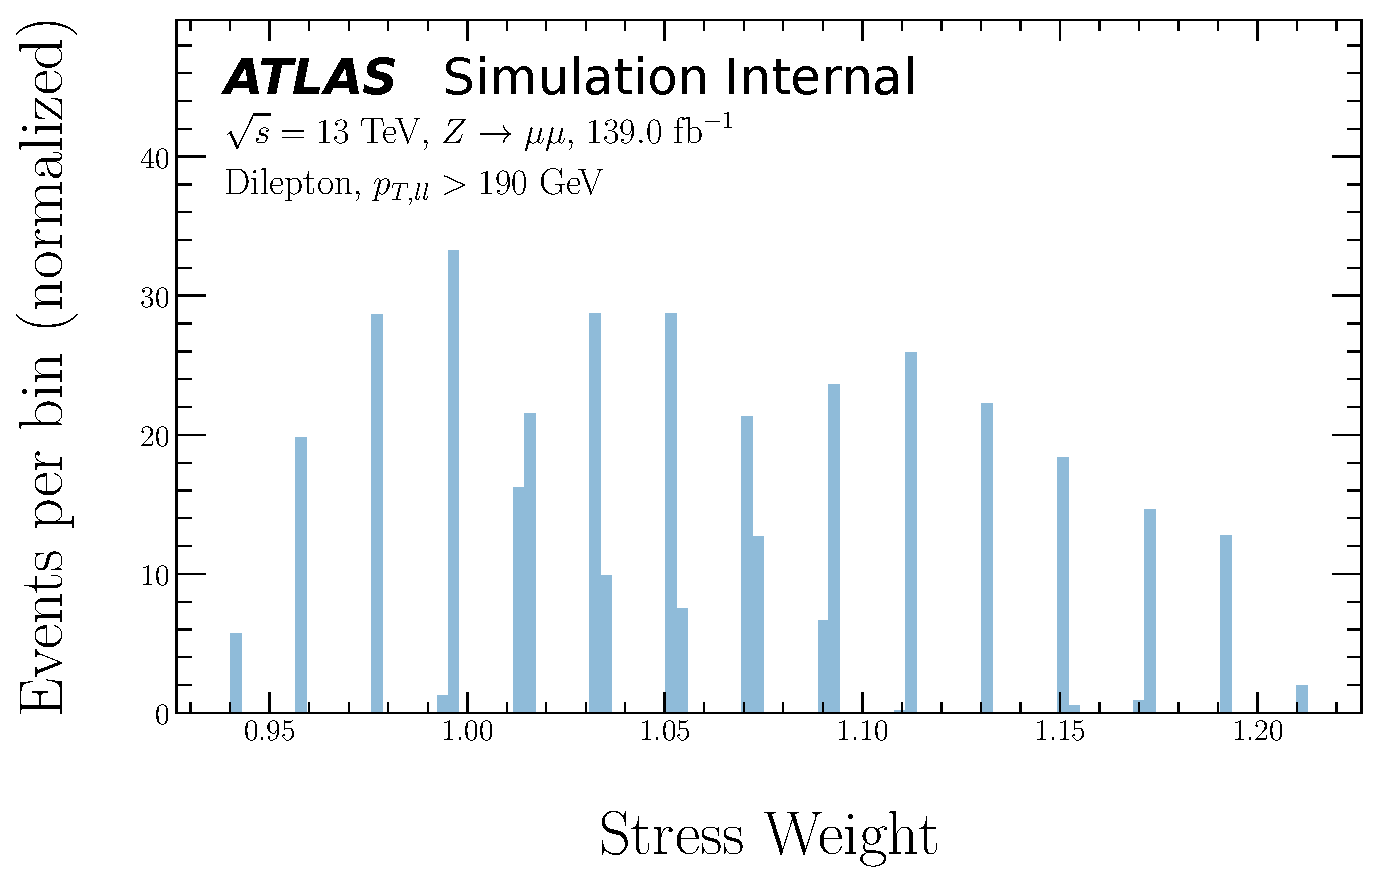
\includegraphics[width=0.45\textwidth]{figures/ATLASOmniFold-StressTest/ATLASOmniFold-StressTestA/UniFold/Ntracks_trackj1/ATLASOmniFold-StressTestA-UniFold-Ntracks_trackj1-StressWeightsHist.pdf}}\\
\subfloat[Input histograms]{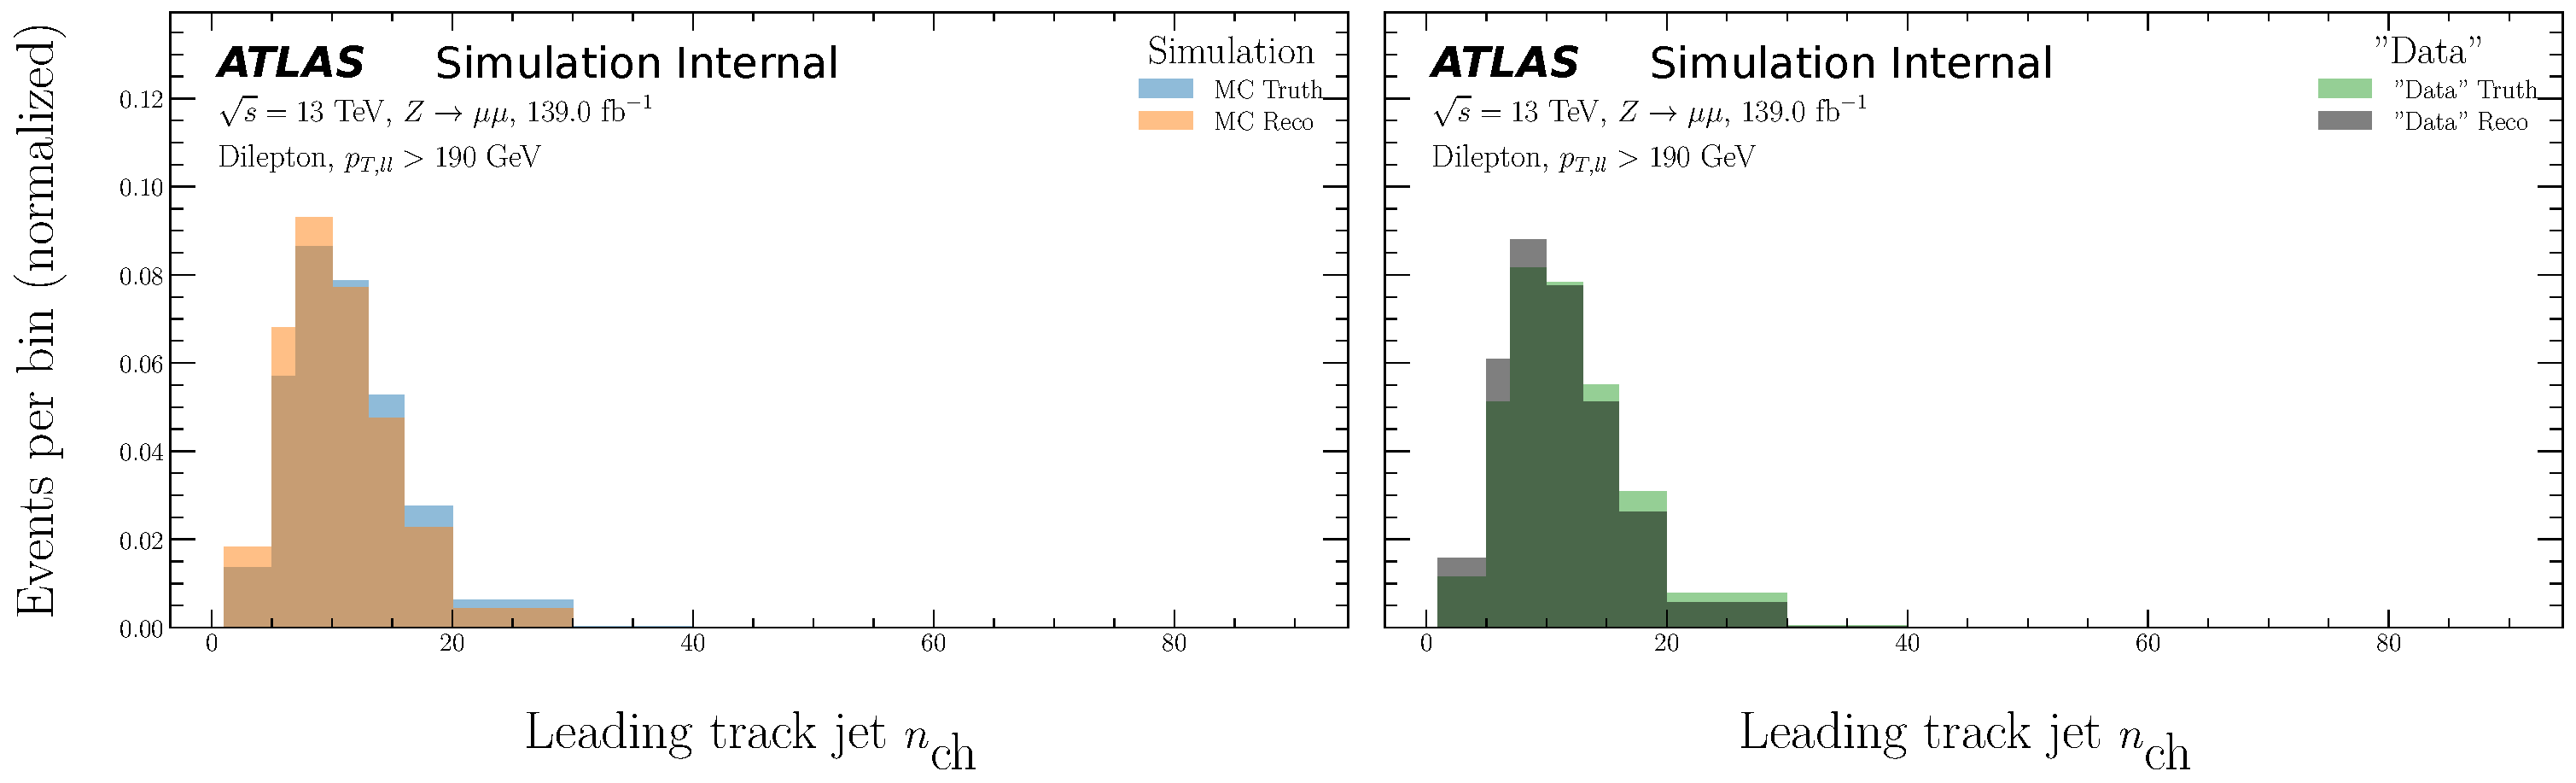
\includegraphics[width=0.85\textwidth]{figures/ATLASOmniFold-StressTest/ATLASOmniFold-StressTestA/UniFold/Ntracks_trackj1/ATLASOmniFold-StressTestA-UniFold-Ntracks_trackj1-Distributions}}\\
\subfloat[After 1 iteration]{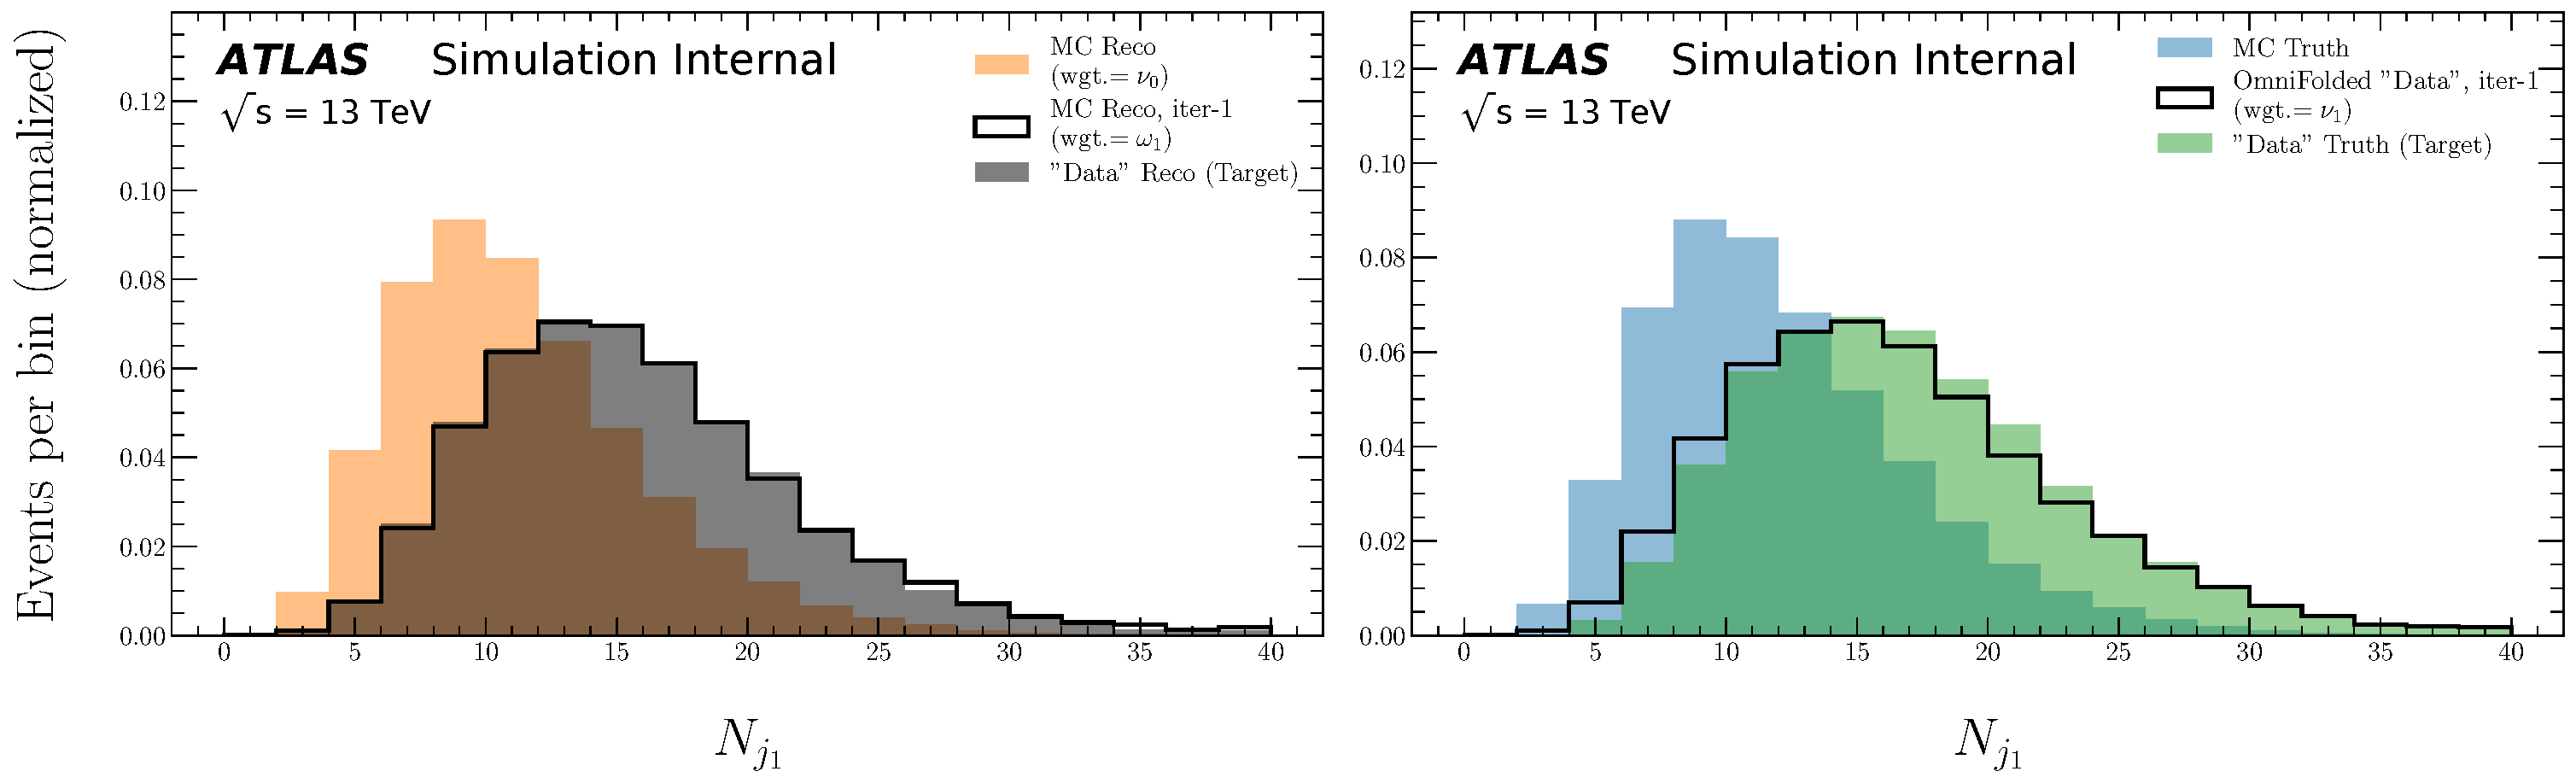
\includegraphics[width=0.85\textwidth]{figures/ATLASOmniFold-StressTest/ATLASOmniFold-StressTestA/UniFold/Ntracks_trackj1/ATLASOmniFold-StressTestA-UniFold-Ntracks_trackj1-Iteration01}}\\
\subfloat[After 2 iterations]{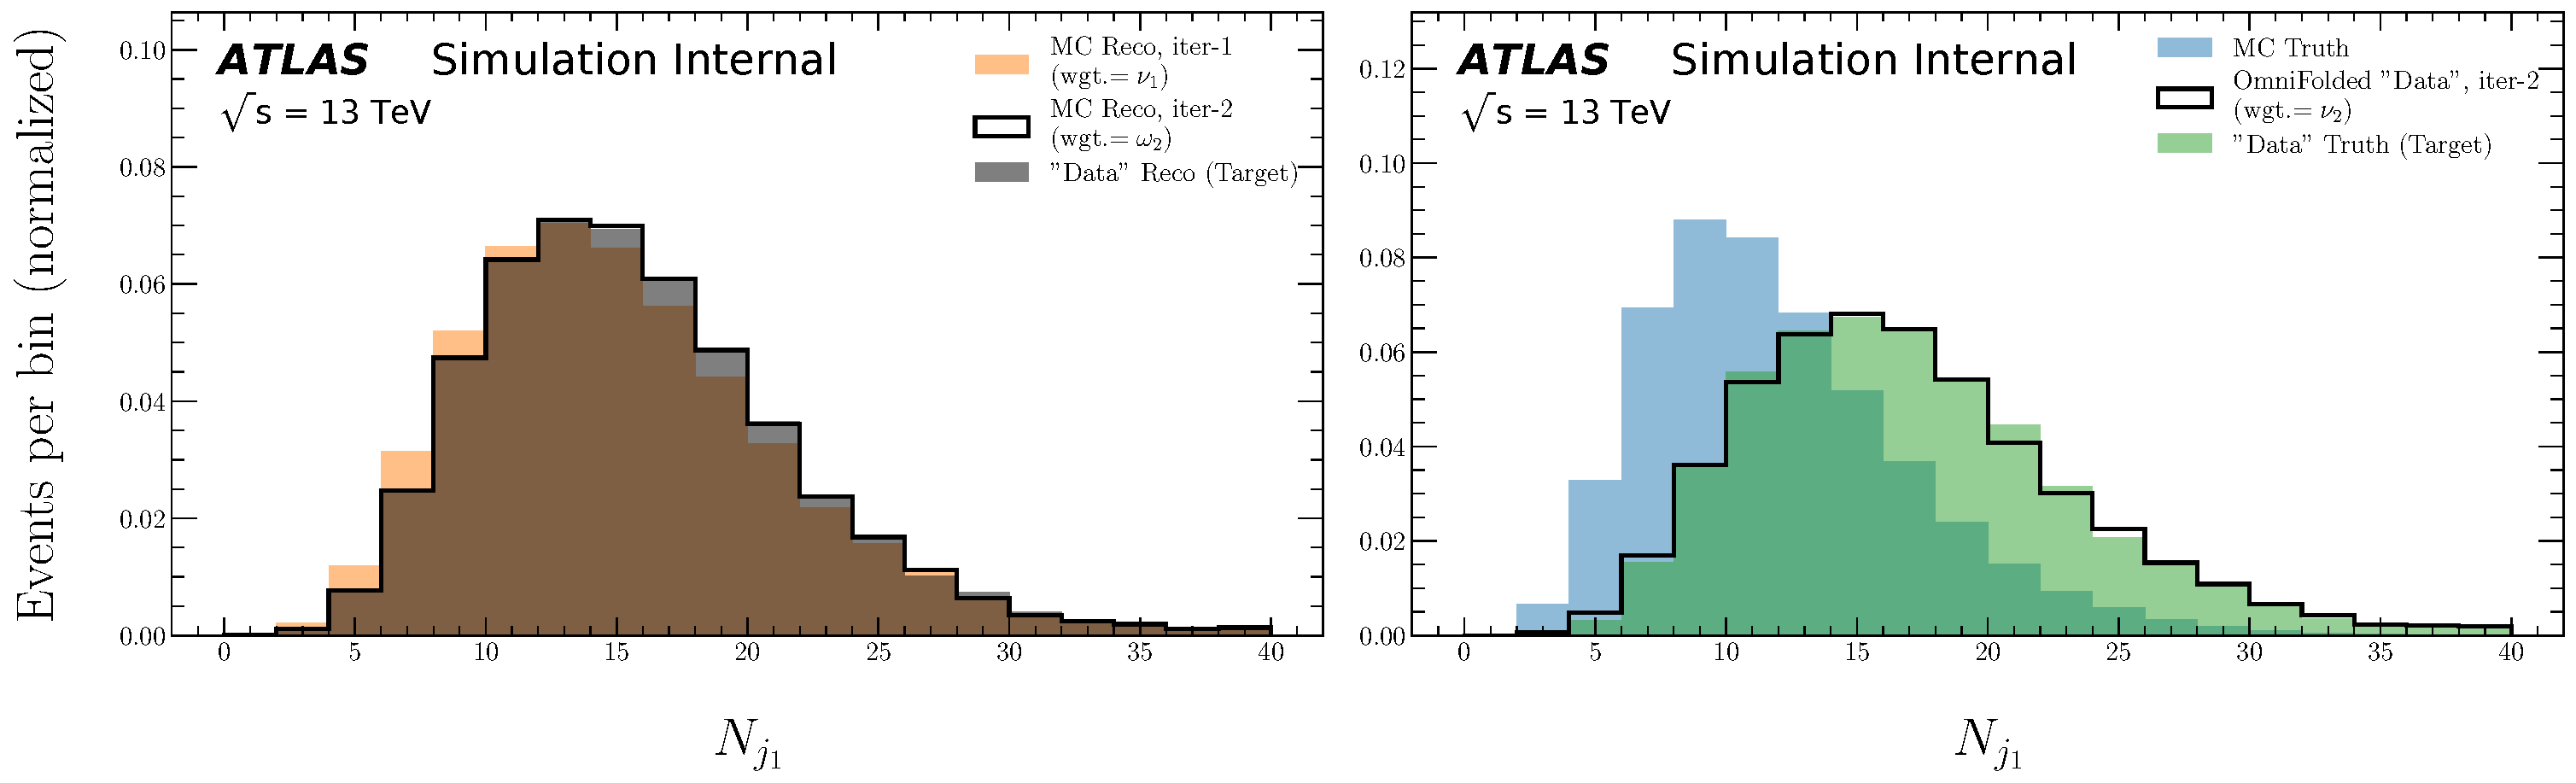
\includegraphics[width=0.85\textwidth]{figures/ATLASOmniFold-StressTest/ATLASOmniFold-StressTestA/UniFold/Ntracks_trackj1/ATLASOmniFold-StressTestA-UniFold-Ntracks_trackj1-Iteration02}}
\phantomcaption 
\end{figure}

\begin{figure}[h!]
\centering
\ContinuedFloat
\subfloat[After 3 iterations]{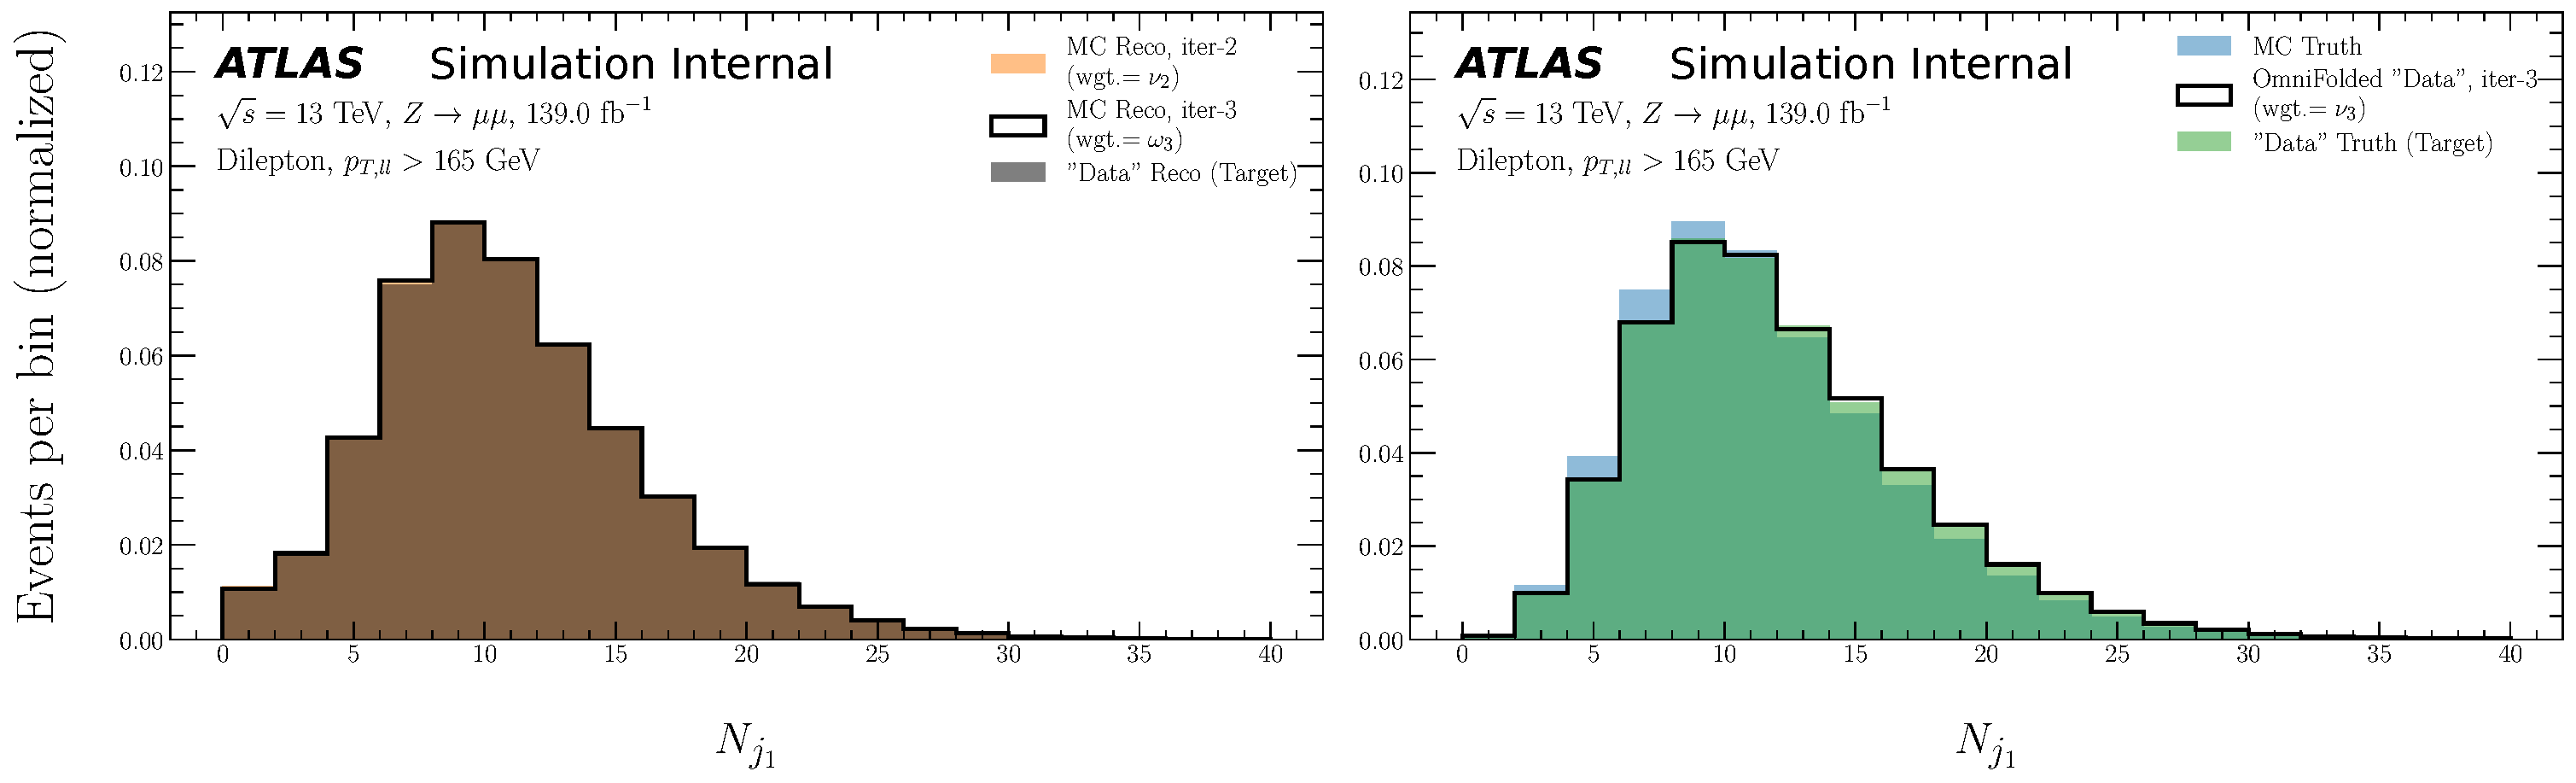
\includegraphics[width=0.85\textwidth]{figures/ATLASOmniFold-StressTest/ATLASOmniFold-StressTestA/UniFold/Ntracks_trackj1/ATLASOmniFold-StressTestA-UniFold-Ntracks_trackj1-Iteration03}}\\
\subfloat[After 4 iterations]{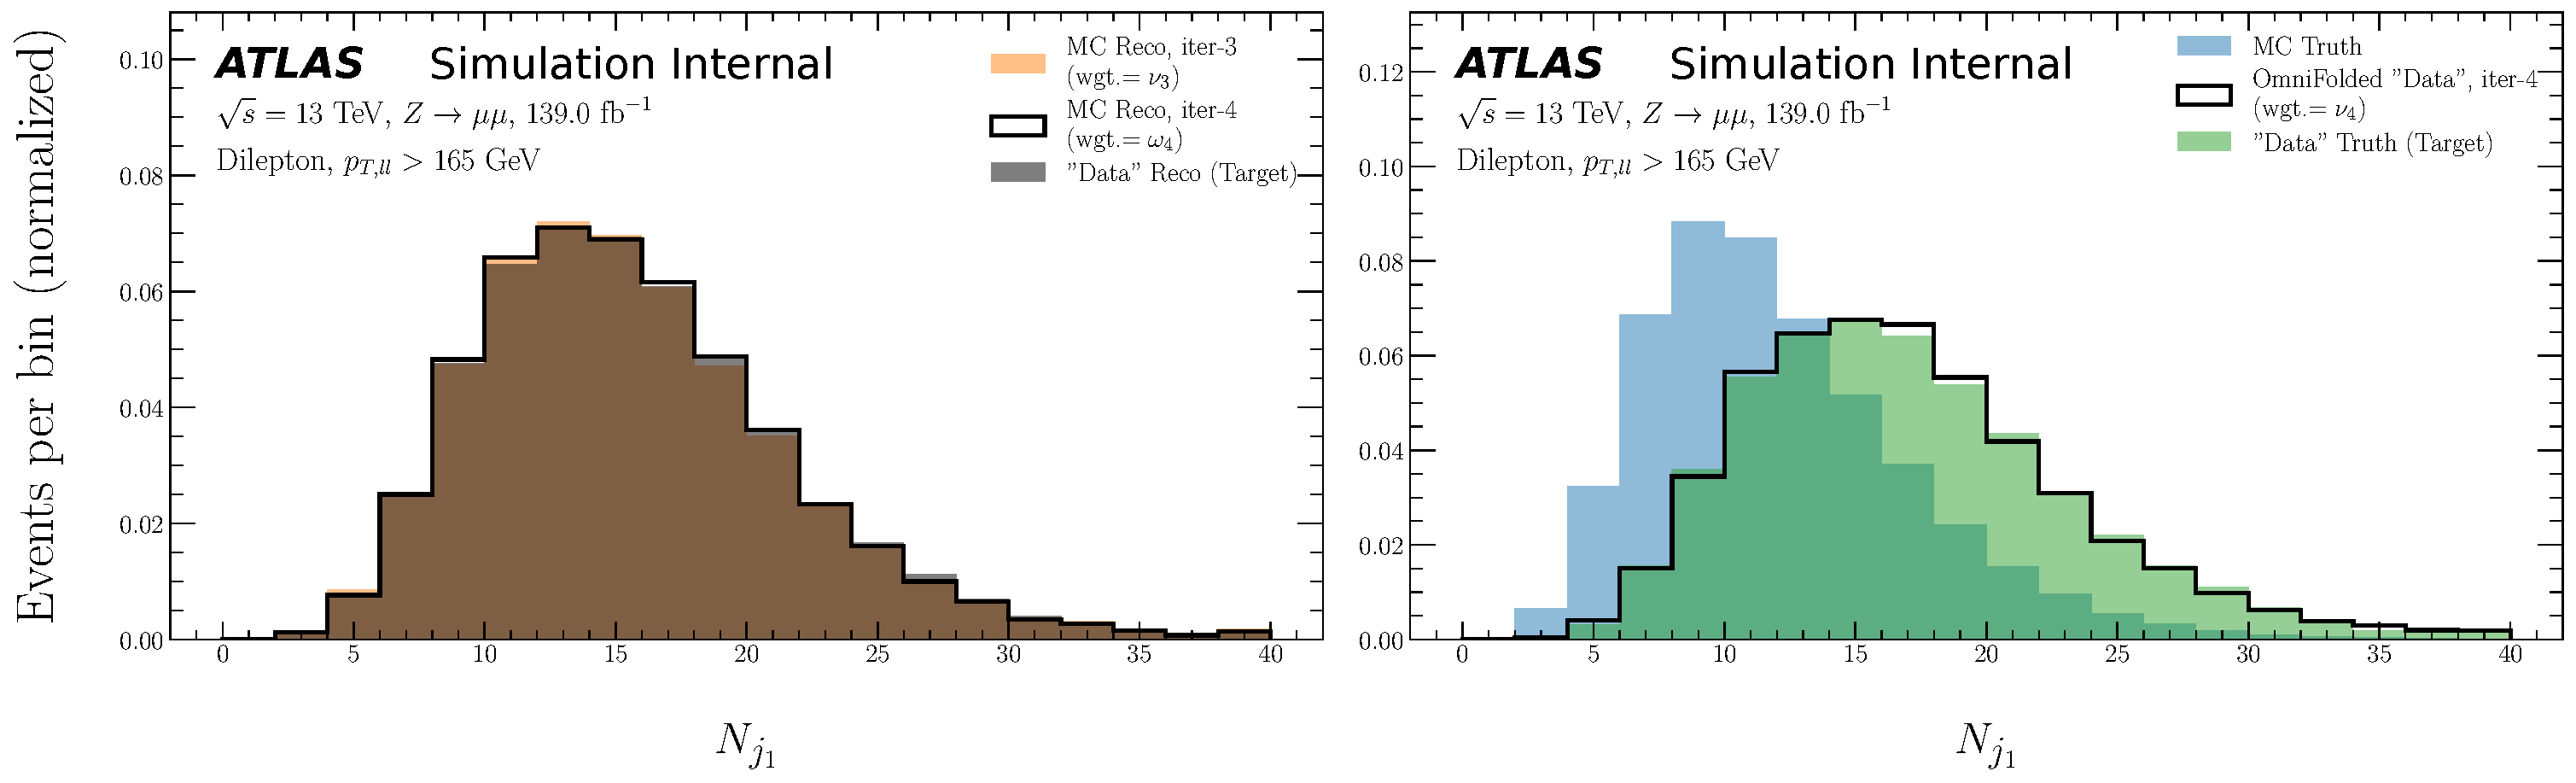
\includegraphics[width=0.85\textwidth]{figures/ATLASOmniFold-StressTest/ATLASOmniFold-StressTestA/UniFold/Ntracks_trackj1/ATLASOmniFold-StressTestA-UniFold-Ntracks_trackj1-Iteration04}}\\
\subfloat[After 5 iterations]{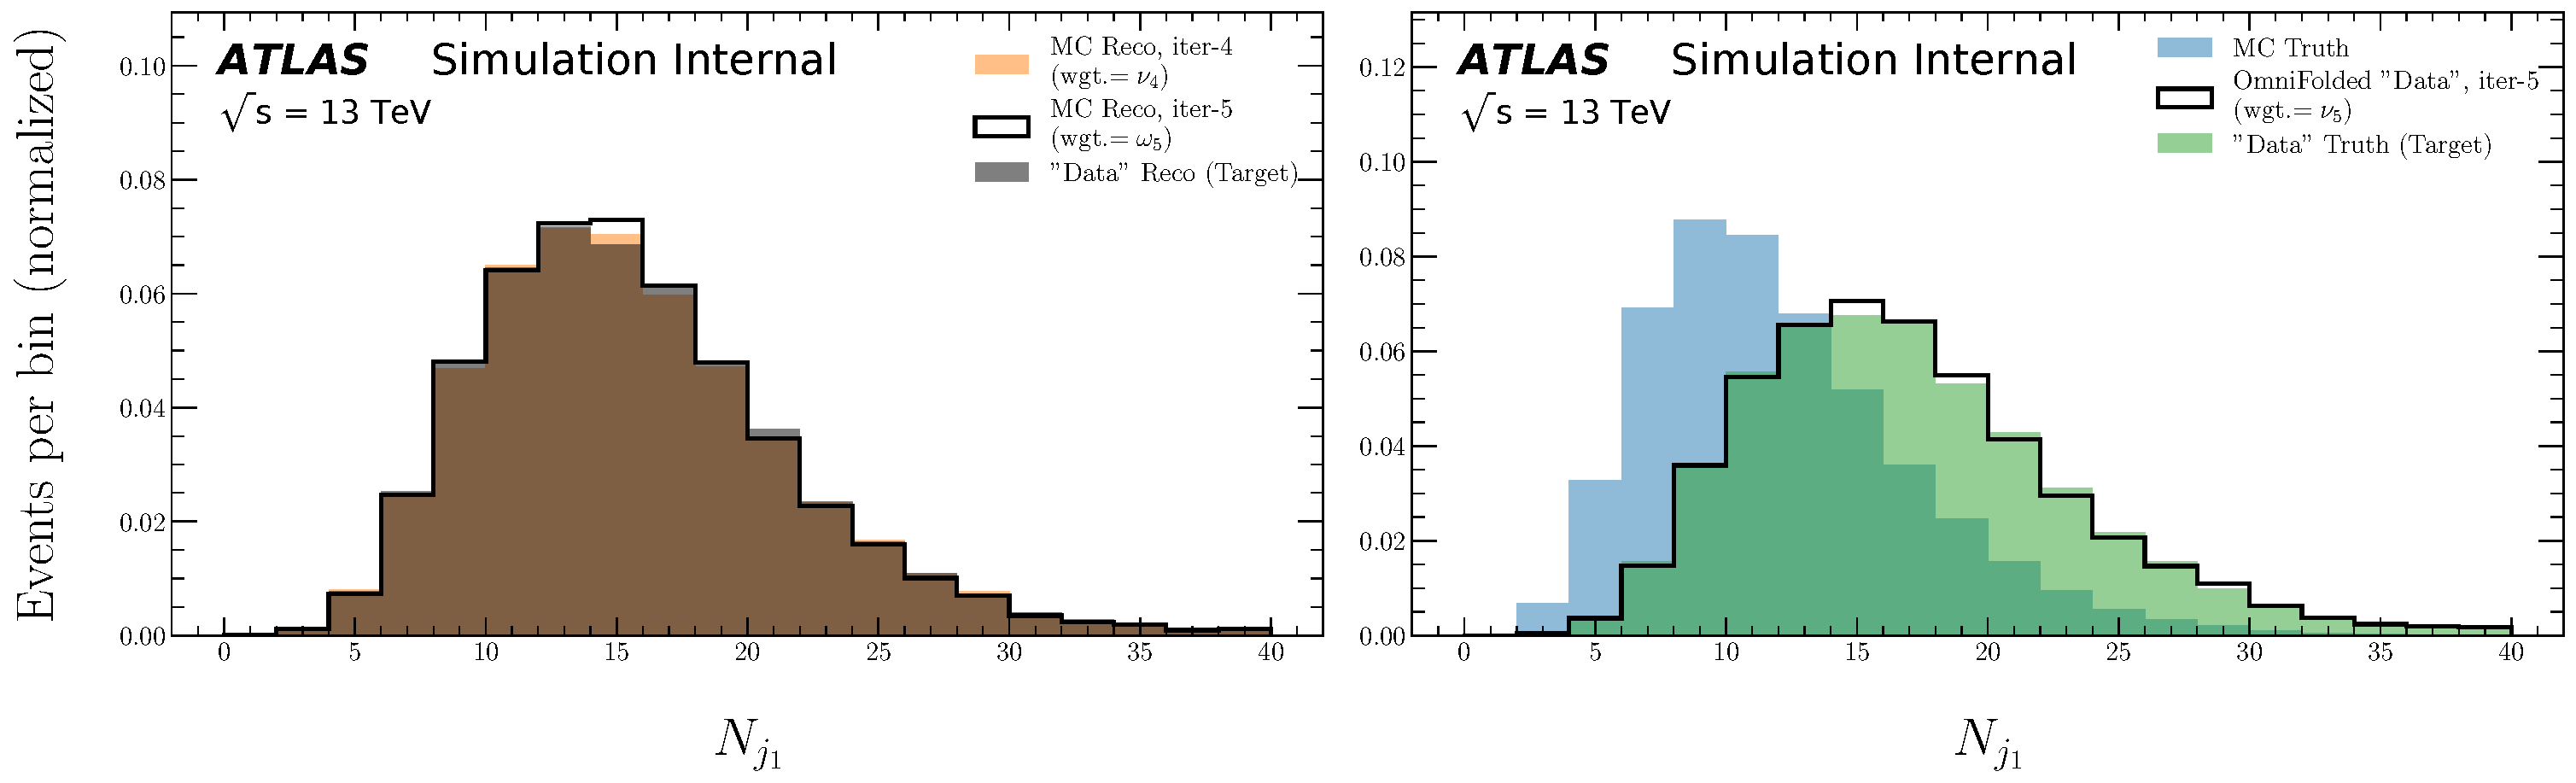
\includegraphics[width=0.85\textwidth]{figures/ATLASOmniFold-StressTest/ATLASOmniFold-StressTestA/UniFold/Ntracks_trackj1/ATLASOmniFold-StressTestA-UniFold-Ntracks_trackj1-Iteration05}}\\
\subfloat[After 6 iterations]{\includegraphics[width=0.85\textwidth]{figures/ATLASOmniFold-StressTest/ATLASOmniFold-StressTestA/UniFold/Ntracks_trackj1/ATLASOmniFold-StressTestA-UniFold-Ntracks_trackj1-Iteration06}}
\caption{A stress test for UniFold applied to the leading track jet constituent multiplicity.}
\label{fig:stressa_Ntracks_trackj1}
\end{figure}

\clearpage

\paragraph{MultiFold} Stress weights for the 16-dimensional MultiFold are shown in Fig.~\ref{fig:stressa_weightsMulti}.  These are constructed by adding the stress weights for each observable as defined by Eq.~\ref{eq:stressweights} (the MC weight only enters once).  Figures~\ref{fig:stressa_massMultih} and~\ref{fig:stressa_Ntracks_trackj1Multi} are examples for the leading track jet mass and the number of tracks inside jets.  Additional examples can be found in App~\ref{sec:stressmultifolddet}.

\begin{figure}[h!]
\centering
\subfloat[Weights]{\includegraphics[width=0.45\textwidth]{figures/ATLASOmniFold-StressTest/ATLASOmniFold-StressTestA/MultiFold/ATLASOmniFold-StressTestA-MultiFold--StressWeightsHist.pdf}}
\caption{A stress weights for the deterministic weight option for MultiFold.  Unlike UniFold, there is now only one set of weights for all 16 observables instead of a different set of weights for each observable.}
\label{fig:stressa_weightsMulti}
\end{figure}

\begin{figure}[h!]
\centering
\subfloat[Input histograms]{\includegraphics[width=0.85\textwidth]{figures/ATLASOmniFold-StressTest/ATLASOmniFold-StressTestA/MultiFold/m_trackj1/ATLASOmniFold-StressTestA-MultiFold-m_trackj1-Distributions}}\\
\subfloat[After 1 iteration]{\includegraphics[width=0.85\textwidth]{figures/ATLASOmniFold-StressTest/ATLASOmniFold-StressTestA/MultiFold/m_trackj1/ATLASOmniFold-StressTestA-MultiFold-m_trackj1-Iteration01}}\\
\subfloat[After 2 iterations]{\includegraphics[width=0.85\textwidth]{figures/ATLASOmniFold-StressTest/ATLASOmniFold-StressTestA/MultiFold/m_trackj1/ATLASOmniFold-StressTestA-MultiFold-m_trackj1-Iteration02}}
\phantomcaption 
\end{figure}

\begin{figure}[h!]
\centering
\ContinuedFloat
\subfloat[After 3 iterations]{\includegraphics[width=0.85\textwidth]{figures/ATLASOmniFold-StressTest/ATLASOmniFold-StressTestA/MultiFold/m_trackj1/ATLASOmniFold-StressTestA-MultiFold-m_trackj1-Iteration03}}\\
\subfloat[After 4 iterations]{\includegraphics[width=0.85\textwidth]{figures/ATLASOmniFold-StressTest/ATLASOmniFold-StressTestA/MultiFold/m_trackj1/ATLASOmniFold-StressTestA-MultiFold-m_trackj1-Iteration04}}\\
\subfloat[After 5 iterations]{\includegraphics[width=0.85\textwidth]{figures/ATLASOmniFold-StressTest/ATLASOmniFold-StressTestA/MultiFold/m_trackj1/ATLASOmniFold-StressTestA-MultiFold-m_trackj1-Iteration05}}\\
\subfloat[After 6 iterations]{\includegraphics[width=0.85\textwidth]{figures/ATLASOmniFold-StressTest/ATLASOmniFold-StressTestA/MultiFold/m_trackj1/ATLASOmniFold-StressTestA-MultiFold-m_trackj1-Iteration06}}
\caption{A stress test for MultiFold using deterministic weights applied to the leading track jet mass.}
\label{fig:stressa_massMultih}
\end{figure}

\begin{figure}[h!]
\centering
\subfloat[Input histograms]{\includegraphics[width=0.85\textwidth]{figures/ATLASOmniFold-StressTest/ATLASOmniFold-StressTestA/MultiFold/Ntracks_trackj1/ATLASOmniFold-StressTestA-MultiFold-Ntracks_trackj1-Distributions}}\\
\subfloat[After 1 iteration]{\includegraphics[width=0.85\textwidth]{figures/ATLASOmniFold-StressTest/ATLASOmniFold-StressTestA/MultiFold/Ntracks_trackj1/ATLASOmniFold-StressTestA-MultiFold-Ntracks_trackj1-Iteration01}}\\
\subfloat[After 2 iterations]{\includegraphics[width=0.85\textwidth]{figures/ATLASOmniFold-StressTest/ATLASOmniFold-StressTestA/MultiFold/Ntracks_trackj1/ATLASOmniFold-StressTestA-MultiFold-Ntracks_trackj1-Iteration02}}
\phantomcaption 
\end{figure}

\begin{figure}[h!]
\centering
\ContinuedFloat
\subfloat[After 3 iterations]{\includegraphics[width=0.85\textwidth]{figures/ATLASOmniFold-StressTest/ATLASOmniFold-StressTestA/MultiFold/Ntracks_trackj1/ATLASOmniFold-StressTestA-MultiFold-Ntracks_trackj1-Iteration03}}\\
\subfloat[After 4 iterations]{\includegraphics[width=0.85\textwidth]{figures/ATLASOmniFold-StressTest/ATLASOmniFold-StressTestA/MultiFold/Ntracks_trackj1/ATLASOmniFold-StressTestA-MultiFold-Ntracks_trackj1-Iteration04}}\\
\subfloat[After 5 iterations]{\includegraphics[width=0.85\textwidth]{figures/ATLASOmniFold-StressTest/ATLASOmniFold-StressTestA/MultiFold/Ntracks_trackj1/ATLASOmniFold-StressTestA-MultiFold-Ntracks_trackj1-Iteration05}}\\
\subfloat[After 6 iterations]{\includegraphics[width=0.85\textwidth]{figures/ATLASOmniFold-StressTest/ATLASOmniFold-StressTestA/MultiFold/Ntracks_trackj1/ATLASOmniFold-StressTestA-MultiFold-Ntracks_trackj1-Iteration06}}
\caption{A stress test for MultiFold using deterministic weights applied to the leading track jet constituent multiplicity.}
\label{fig:stressa_Ntracks_trackj1Multi}
\end{figure}

\clearpage

\subsubsection{Stochastic Weights}
\label{sec:stress:stochastic}

For a given event $x$ in sample $X$, the stress weights are given by 

\begin{align}
\label{eq:stressBweights}
w = w_{MC}\,|\mathcal{N}(0, \sigma((\mathcal{Z}(x))))|\,,
\end{align}
%
where $w_{MC}$ is the Monte Carlo event weight, $\mathcal{Z}$ gives the z-score of $x\in X$, and $\sigma$ is the sigmoid function $\sigma(x)=\frac{1}{1 + e^{-x}}$.  We do a basic weight standardization given all stress weights $W$ by doing $w\mapsto\frac{w}{\langle W\rangle}$. These stress weights are constructed to induce a right shift in the given distribution.  Note these stress weights are based on a random variable, unlike the ones in Sec.~\ref{sec:stress:deterministic}.

\paragraph{UniFold}

Figures~\ref{fig:stressb_mass} and~\ref{fig:stressb_Ntracks_trackj1} are examples for the leading track jet mass and the number of tracks inside jets.  Additional examples can be found in App~\ref{sec:stressBunifolddet}.

\begin{figure}[h!]
\centering
\subfloat[Weights]{\includegraphics[width=0.45\textwidth]{figures/ATLASOmniFold-StressTest/ATLASOmniFold-StressTestB/UniFold/m_trackj1/ATLASOmniFold-StressTestB-UniFold-m_trackj1-StressWeightsHist.pdf}}\\
\subfloat[Input histograms]{\includegraphics[width=0.85\textwidth]{figures/ATLASOmniFold-StressTest/ATLASOmniFold-StressTestB/UniFold/m_trackj1/ATLASOmniFold-StressTestB-UniFold-m_trackj1-Distributions}}\\
\subfloat[After 1 iteration]{\includegraphics[width=0.85\textwidth]{figures/ATLASOmniFold-StressTest/ATLASOmniFold-StressTestB/UniFold/m_trackj1/ATLASOmniFold-StressTestB-UniFold-m_trackj1-Iteration01}}\\
\subfloat[After 2 iterations]{\includegraphics[width=0.85\textwidth]{figures/ATLASOmniFold-StressTest/ATLASOmniFold-StressTestB/UniFold/m_trackj1/ATLASOmniFold-StressTestB-UniFold-m_trackj1-Iteration02}}
\phantomcaption 
\end{figure}

\begin{figure}[h!]
\centering
\ContinuedFloat
\subfloat[After 3 iterations]{\includegraphics[width=0.85\textwidth]{figures/ATLASOmniFold-StressTest/ATLASOmniFold-StressTestB/UniFold/m_trackj1/ATLASOmniFold-StressTestB-UniFold-m_trackj1-Iteration03}}\\
\subfloat[After 4 iterations]{\includegraphics[width=0.85\textwidth]{figures/ATLASOmniFold-StressTest/ATLASOmniFold-StressTestB/UniFold/m_trackj1/ATLASOmniFold-StressTestB-UniFold-m_trackj1-Iteration04}}\\
\subfloat[After 5 iterations]{\includegraphics[width=0.85\textwidth]{figures/ATLASOmniFold-StressTest/ATLASOmniFold-StressTestB/UniFold/m_trackj1/ATLASOmniFold-StressTestB-UniFold-m_trackj1-Iteration05}}\\
\subfloat[After 6 iterations]{\includegraphics[width=0.85\textwidth]{figures/ATLASOmniFold-StressTest/ATLASOmniFold-StressTestB/UniFold/m_trackj1/ATLASOmniFold-StressTestB-UniFold-m_trackj1-Iteration06}}
\caption{A stress test for UniFold applied to the leading track jet mass.}
\label{fig:stressb_mass}
\end{figure}

\begin{figure}[h!]
\centering
\subfloat[Weights]{\includegraphics[width=0.45\textwidth]{figures/ATLASOmniFold-StressTest/ATLASOmniFold-StressTestB/UniFold/Ntracks_trackj1/ATLASOmniFold-StressTestB-UniFold-Ntracks_trackj1-StressWeightsHist.pdf}}\\
\subfloat[Input histograms]{\includegraphics[width=0.85\textwidth]{figures/ATLASOmniFold-StressTest/ATLASOmniFold-StressTestB/UniFold/Ntracks_trackj1/ATLASOmniFold-StressTestB-UniFold-Ntracks_trackj1-Distributions}}\\
\subfloat[After 1 iteration]{\includegraphics[width=0.85\textwidth]{figures/ATLASOmniFold-StressTest/ATLASOmniFold-StressTestB/UniFold/Ntracks_trackj1/ATLASOmniFold-StressTestB-UniFold-Ntracks_trackj1-Iteration01}}\\
\subfloat[After 2 iterations]{\includegraphics[width=0.85\textwidth]{figures/ATLASOmniFold-StressTest/ATLASOmniFold-StressTestB/UniFold/Ntracks_trackj1/ATLASOmniFold-StressTestB-UniFold-Ntracks_trackj1-Iteration02}}
\phantomcaption 
\end{figure}

\begin{figure}[h!]
\centering
\ContinuedFloat
\subfloat[After 3 iterations]{\includegraphics[width=0.85\textwidth]{figures/ATLASOmniFold-StressTest/ATLASOmniFold-StressTestB/UniFold/Ntracks_trackj1/ATLASOmniFold-StressTestB-UniFold-Ntracks_trackj1-Iteration03}}\\
\subfloat[After 4 iterations]{\includegraphics[width=0.85\textwidth]{figures/ATLASOmniFold-StressTest/ATLASOmniFold-StressTestB/UniFold/Ntracks_trackj1/ATLASOmniFold-StressTestB-UniFold-Ntracks_trackj1-Iteration04}}\\
\subfloat[After 5 iterations]{\includegraphics[width=0.85\textwidth]{figures/ATLASOmniFold-StressTest/ATLASOmniFold-StressTestB/UniFold/Ntracks_trackj1/ATLASOmniFold-StressTestB-UniFold-Ntracks_trackj1-Iteration05}}\\
\subfloat[After 6 iterations]{\includegraphics[width=0.85\textwidth]{figures/ATLASOmniFold-StressTest/ATLASOmniFold-StressTestB/UniFold/Ntracks_trackj1/ATLASOmniFold-StressTestB-UniFold-Ntracks_trackj1-Iteration06}}
\caption{A stress test for UniFold applied to the leading track jet constituent multiplicity.}
\label{fig:stressb_Ntracks_trackj1}
\end{figure}

\clearpage

\paragraph{MultiFold} Stress weights for the 16-dimensional MultiFold are shown in Fig.~\ref{fig:stressb_weightsMulti}.  These are constructed by adding the stress weights for each observable as defined by Eq.~\ref{eq:stressBweights} (the MC weight only enters once).  Figures~\ref{fig:stressb_massMultih} and~\ref{fig:stressb_Ntracks_trackj1Multi} are examples for the leading track jet mass and the number of tracks inside jets.  Additional examples can be found in App~\ref{sec:stressBmultifolddet}.

\begin{figure}[h!]
\centering
\subfloat[Weights]{\includegraphics[width=0.45\textwidth]{figures/ATLASOmniFold-StressTest/ATLASOmniFold-StressTestB/MultiFold/ATLASOmniFold-StressTestB-MultiFold--StressWeightsHist.pdf}}
\caption{A stress weights for the deterministic weight option for MultiFold.  Unlike UniFold, there is now only one set of weights for all 16 observables instead of a different set of weights for each observable.}
\label{fig:stressb_weightsMulti}
\end{figure}

\begin{figure}[h!]
\centering
\subfloat[Input histograms]{\includegraphics[width=0.85\textwidth]{figures/ATLASOmniFold-StressTest/ATLASOmniFold-StressTestB/MultiFold/m_trackj1/ATLASOmniFold-StressTestB-MultiFold-m_trackj1-Distributions}}\\
\subfloat[After 1 iteration]{\includegraphics[width=0.85\textwidth]{figures/ATLASOmniFold-StressTest/ATLASOmniFold-StressTestB/MultiFold/m_trackj1/ATLASOmniFold-StressTestB-MultiFold-m_trackj1-Iteration01}}\\
\subfloat[After 2 iterations]{\includegraphics[width=0.85\textwidth]{figures/ATLASOmniFold-StressTest/ATLASOmniFold-StressTestB/MultiFold/m_trackj1/ATLASOmniFold-StressTestB-MultiFold-m_trackj1-Iteration02}}
\phantomcaption 
\end{figure}

\begin{figure}[h!]
\centering
\ContinuedFloat
\subfloat[After 3 iterations]{\includegraphics[width=0.85\textwidth]{figures/ATLASOmniFold-StressTest/ATLASOmniFold-StressTestB/MultiFold/m_trackj1/ATLASOmniFold-StressTestB-MultiFold-m_trackj1-Iteration03}}\\
\subfloat[After 4 iterations]{\includegraphics[width=0.85\textwidth]{figures/ATLASOmniFold-StressTest/ATLASOmniFold-StressTestB/MultiFold/m_trackj1/ATLASOmniFold-StressTestB-MultiFold-m_trackj1-Iteration04}}\\
\subfloat[After 5 iterations]{\includegraphics[width=0.85\textwidth]{figures/ATLASOmniFold-StressTest/ATLASOmniFold-StressTestB/MultiFold/m_trackj1/ATLASOmniFold-StressTestB-MultiFold-m_trackj1-Iteration05}}\\
\subfloat[After 6 iterations]{\includegraphics[width=0.85\textwidth]{figures/ATLASOmniFold-StressTest/ATLASOmniFold-StressTestB/MultiFold/m_trackj1/ATLASOmniFold-StressTestB-MultiFold-m_trackj1-Iteration06}}
\caption{A stress test for MultiFold using deterministic weights applied to the leading track jet mass.}
\label{fig:stressb_massMultih}
\end{figure}

\begin{figure}[h!]
\centering
\subfloat[Input histograms]{\includegraphics[width=0.85\textwidth]{figures/ATLASOmniFold-StressTest/ATLASOmniFold-StressTestB/MultiFold/Ntracks_trackj1/ATLASOmniFold-StressTestB-MultiFold-Ntracks_trackj1-Distributions}}\\
\subfloat[After 1 iteration]{\includegraphics[width=0.85\textwidth]{figures/ATLASOmniFold-StressTest/ATLASOmniFold-StressTestB/MultiFold/Ntracks_trackj1/ATLASOmniFold-StressTestB-MultiFold-Ntracks_trackj1-Iteration01}}\\
\subfloat[After 2 iterations]{\includegraphics[width=0.85\textwidth]{figures/ATLASOmniFold-StressTest/ATLASOmniFold-StressTestB/MultiFold/Ntracks_trackj1/ATLASOmniFold-StressTestB-MultiFold-Ntracks_trackj1-Iteration02}}
\phantomcaption 
\end{figure}

\begin{figure}[h!]
\centering
\ContinuedFloat
\subfloat[After 3 iterations]{\includegraphics[width=0.85\textwidth]{figures/ATLASOmniFold-StressTest/ATLASOmniFold-StressTestB/MultiFold/Ntracks_trackj1/ATLASOmniFold-StressTestB-MultiFold-Ntracks_trackj1-Iteration03}}\\
\subfloat[After 4 iterations]{\includegraphics[width=0.85\textwidth]{figures/ATLASOmniFold-StressTest/ATLASOmniFold-StressTestB/MultiFold/Ntracks_trackj1/ATLASOmniFold-StressTestB-MultiFold-Ntracks_trackj1-Iteration04}}\\
\subfloat[After 5 iterations]{\includegraphics[width=0.85\textwidth]{figures/ATLASOmniFold-StressTest/ATLASOmniFold-StressTestB/MultiFold/Ntracks_trackj1/ATLASOmniFold-StressTestB-MultiFold-Ntracks_trackj1-Iteration05}}\\
\subfloat[After 6 iterations]{\includegraphics[width=0.85\textwidth]{figures/ATLASOmniFold-StressTest/ATLASOmniFold-StressTestB/MultiFold/Ntracks_trackj1/ATLASOmniFold-StressTestB-MultiFold-Ntracks_trackj1-Iteration06}}
\caption{A stress test for MultiFold using deterministic weights applied to the leading track jet constituent multiplicity.}
\label{fig:stressb_Ntracks_trackj1Multi}
\end{figure}

\clearpage

\subsection{Model Dependence}
\label{sec:modeldep}

In this section, we unfold Sherpa with Pythia.

\paragraph{UniFold}

Figures~\ref{fig:stressc_mass} and~\ref{fig:stressc_Ntracks_trackj1} are examples for the leading track jet mass and the number of tracks inside jets.  Additional examples can be found in App~\ref{sec:stresscunifolddet}.

\begin{figure}[h!]
\centering
\subfloat[Input histograms]{\includegraphics[width=0.85\textwidth]{figures/ATLASOmniFold-StressTest/ATLASOmniFold-StressTestC/UniFold/m_trackj1/ATLASOmniFold-StressTestC-UniFold-m_trackj1-Distributions}}\\
\subfloat[After 1 iteration]{\includegraphics[width=0.85\textwidth]{figures/ATLASOmniFold-StressTest/ATLASOmniFold-StressTestC/UniFold/m_trackj1/ATLASOmniFold-StressTestC-UniFold-m_trackj1-Iteration01}}\\
\subfloat[After 2 iterations]{\includegraphics[width=0.85\textwidth]{figures/ATLASOmniFold-StressTest/ATLASOmniFold-StressTestC/UniFold/m_trackj1/ATLASOmniFold-StressTestC-UniFold-m_trackj1-Iteration02}}
\phantomcaption 
\end{figure}

\begin{figure}[h!]
\centering
\ContinuedFloat
\subfloat[After 3 iterations]{\includegraphics[width=0.85\textwidth]{figures/ATLASOmniFold-StressTest/ATLASOmniFold-StressTestC/UniFold/m_trackj1/ATLASOmniFold-StressTestC-UniFold-m_trackj1-Iteration03}}\\
\subfloat[After 4 iterations]{\includegraphics[width=0.85\textwidth]{figures/ATLASOmniFold-StressTest/ATLASOmniFold-StressTestC/UniFold/m_trackj1/ATLASOmniFold-StressTestC-UniFold-m_trackj1-Iteration04}}\\
\subfloat[After 5 iterations]{\includegraphics[width=0.85\textwidth]{figures/ATLASOmniFold-StressTest/ATLASOmniFold-StressTestC/UniFold/m_trackj1/ATLASOmniFold-StressTestC-UniFold-m_trackj1-Iteration05}}\\
\subfloat[After 6 iterations]{\includegraphics[width=0.85\textwidth]{figures/ATLASOmniFold-StressTest/ATLASOmniFold-StressTestC/UniFold/m_trackj1/ATLASOmniFold-StressTestC-UniFold-m_trackj1-Iteration06}}
\caption{UniFolding Sherpa with Pythia for the leading track jet mass.}
\label{fig:stressc_mass}
\end{figure}

\begin{figure}[h!]
\centering
\subfloat[Input histograms]{\includegraphics[width=0.85\textwidth]{figures/ATLASOmniFold-StressTest/ATLASOmniFold-StressTestC/UniFold/Ntracks_trackj1/ATLASOmniFold-StressTestC-UniFold-Ntracks_trackj1-Distributions}}\\
\subfloat[After 1 iteration]{\includegraphics[width=0.85\textwidth]{figures/ATLASOmniFold-StressTest/ATLASOmniFold-StressTestC/UniFold/Ntracks_trackj1/ATLASOmniFold-StressTestC-UniFold-Ntracks_trackj1-Iteration01}}\\
\subfloat[After 2 iterations]{\includegraphics[width=0.85\textwidth]{figures/ATLASOmniFold-StressTest/ATLASOmniFold-StressTestC/UniFold/Ntracks_trackj1/ATLASOmniFold-StressTestC-UniFold-Ntracks_trackj1-Iteration02}}
\phantomcaption 
\end{figure}

\begin{figure}[h!]
\centering
\ContinuedFloat
\subfloat[After 3 iterations]{\includegraphics[width=0.85\textwidth]{figures/ATLASOmniFold-StressTest/ATLASOmniFold-StressTestC/UniFold/Ntracks_trackj1/ATLASOmniFold-StressTestC-UniFold-Ntracks_trackj1-Iteration03}}\\
\subfloat[After 4 iterations]{\includegraphics[width=0.85\textwidth]{figures/ATLASOmniFold-StressTest/ATLASOmniFold-StressTestC/UniFold/Ntracks_trackj1/ATLASOmniFold-StressTestC-UniFold-Ntracks_trackj1-Iteration04}}\\
\subfloat[After 5 iterations]{\includegraphics[width=0.85\textwidth]{figures/ATLASOmniFold-StressTest/ATLASOmniFold-StressTestC/UniFold/Ntracks_trackj1/ATLASOmniFold-StressTestC-UniFold-Ntracks_trackj1-Iteration05}}\\
\subfloat[After 6 iterations]{\includegraphics[width=0.85\textwidth]{figures/ATLASOmniFold-StressTest/ATLASOmniFold-StressTestC/UniFold/Ntracks_trackj1/ATLASOmniFold-StressTestC-UniFold-Ntracks_trackj1-Iteration06}}
\caption{UniFolding Sherpa with Pythia forthe leading track jet constituent multiplicity.}
\label{fig:stressc_Ntracks_trackj1}
\end{figure}

\clearpage

\paragraph{MultiFold} Figures~\ref{fig:stressc_massMultih} and~\ref{fig:stressc_Ntracks_trackj1Multi} are examples for the leading track jet mass and the number of tracks inside jets.  Additional examples can be found in App~\ref{sec:stresscmultifolddet}.

\begin{figure}[h!]
\centering
\subfloat[Input histograms]{\includegraphics[width=0.85\textwidth]{figures/ATLASOmniFold-StressTest/ATLASOmniFold-StressTestC/MultiFold/m_trackj1/ATLASOmniFold-StressTestC-MultiFold-m_trackj1-Distributions}}\\
\subfloat[After 1 iteration]{\includegraphics[width=0.85\textwidth]{figures/ATLASOmniFold-StressTest/ATLASOmniFold-StressTestC/MultiFold/m_trackj1/ATLASOmniFold-StressTestC-MultiFold-m_trackj1-Iteration01}}\\
\subfloat[After 2 iterations]{\includegraphics[width=0.85\textwidth]{figures/ATLASOmniFold-StressTest/ATLASOmniFold-StressTestC/MultiFold/m_trackj1/ATLASOmniFold-StressTestC-MultiFold-m_trackj1-Iteration02}}
\phantomcaption 
\end{figure}

\begin{figure}[h!]
\centering
\ContinuedFloat
\subfloat[After 3 iterations]{\includegraphics[width=0.85\textwidth]{figures/ATLASOmniFold-StressTest/ATLASOmniFold-StressTestC/MultiFold/m_trackj1/ATLASOmniFold-StressTestC-MultiFold-m_trackj1-Iteration03}}\\
\subfloat[After 4 iterations]{\includegraphics[width=0.85\textwidth]{figures/ATLASOmniFold-StressTest/ATLASOmniFold-StressTestC/MultiFold/m_trackj1/ATLASOmniFold-StressTestC-MultiFold-m_trackj1-Iteration04}}\\
\subfloat[After 5 iterations]{\includegraphics[width=0.85\textwidth]{figures/ATLASOmniFold-StressTest/ATLASOmniFold-StressTestC/MultiFold/m_trackj1/ATLASOmniFold-StressTestC-MultiFold-m_trackj1-Iteration05}}\\
\subfloat[After 6 iterations]{\includegraphics[width=0.85\textwidth]{figures/ATLASOmniFold-StressTest/ATLASOmniFold-StressTestC/MultiFold/m_trackj1/ATLASOmniFold-StressTestC-MultiFold-m_trackj1-Iteration06}}
\caption{MultiFolding Sherpa with Pythia for the leading track jet mass.}
\label{fig:stressc_massMultih}
\end{figure}

\begin{figure}[h!]
\centering
\subfloat[Input histograms]{\includegraphics[width=0.85\textwidth]{figures/ATLASOmniFold-StressTest/ATLASOmniFold-StressTestC/MultiFold/Ntracks_trackj1/ATLASOmniFold-StressTestC-MultiFold-Ntracks_trackj1-Distributions}}\\
\subfloat[After 1 iteration]{\includegraphics[width=0.85\textwidth]{figures/ATLASOmniFold-StressTest/ATLASOmniFold-StressTestC/MultiFold/Ntracks_trackj1/ATLASOmniFold-StressTestC-MultiFold-Ntracks_trackj1-Iteration01}}\\
\subfloat[After 2 iterations]{\includegraphics[width=0.85\textwidth]{figures/ATLASOmniFold-StressTest/ATLASOmniFold-StressTestC/MultiFold/Ntracks_trackj1/ATLASOmniFold-StressTestC-MultiFold-Ntracks_trackj1-Iteration02}}
\phantomcaption 
\end{figure}

\begin{figure}[h!]
\centering
\ContinuedFloat
\subfloat[After 3 iterations]{\includegraphics[width=0.85\textwidth]{figures/ATLASOmniFold-StressTest/ATLASOmniFold-StressTestC/MultiFold/Ntracks_trackj1/ATLASOmniFold-StressTestC-MultiFold-Ntracks_trackj1-Iteration03}}\\
\subfloat[After 4 iterations]{\includegraphics[width=0.85\textwidth]{figures/ATLASOmniFold-StressTest/ATLASOmniFold-StressTestC/MultiFold/Ntracks_trackj1/ATLASOmniFold-StressTestC-MultiFold-Ntracks_trackj1-Iteration04}}\\
\subfloat[After 5 iterations]{\includegraphics[width=0.85\textwidth]{figures/ATLASOmniFold-StressTest/ATLASOmniFold-StressTestC/MultiFold/Ntracks_trackj1/ATLASOmniFold-StressTestC-MultiFold-Ntracks_trackj1-Iteration05}}\\
\subfloat[After 6 iterations]{\includegraphics[width=0.85\textwidth]{figures/ATLASOmniFold-StressTest/ATLASOmniFold-StressTestC/MultiFold/Ntracks_trackj1/ATLASOmniFold-StressTestC-MultiFold-Ntracks_trackj1-Iteration06}}
\caption{MultiFolding Sherpa with Pythia for the leading track jet constituent multiplicity.}
\label{fig:stressc_Ntracks_trackj1Multi}
\end{figure}
